\documentclass{beamer}


\usepackage[spanish]{babel} 
\usepackage[utf8]{inputenc} 
\usepackage{amsmath}
\usepackage{hyperref}
\usepackage[nodayofweek]{datetime}
\usepackage{pgfpages}

\usepackage{caption}
\usepackage{subcaption}

\makeatletter
\def\verbatim@font{\ttfamily\tiny}
\makeatother

%~ \usetheme{Berkeley}
%~ \usetheme{CambridgeUS} %~ Ok 3
%~ \usetheme{Boadilla} %~ Ok 2
\usetheme{boxes} %~ Ok 1
\setbeamerfont{frametitle}{size=\small}

\usecolortheme{seahorse} %~ OK
%~ \usecolortheme{dolphin} 
%~ \usecolortheme{beaver}
%~ \usecolortheme{whale}
%~ \usecolortheme{lily}


%~ \usetheme{Frankfurt}
%~ \usetheme{Madrid}
%~ \usetheme{Malmoe}

%~ \setbeamercovered{transparent}

\logo{%
	   
\includegraphics[scale=.25]{img/logoIBR2016_byn.png}
   }
\title[]{Estudios sobre la regulación de la expresión génica por microARNs en plantas mediante estrategias bioinformáticas}

\author{Uciel Chorostecki}
\institute[IBR]{ \\Director Dr. Javier Palatnik\\Instituto Biología Molecular y Celular Rosario}
\date{}

\begin{document}

\frame{\titlepage}

\section{Introducción}

\begin{frame}{MicroARNs}
    %~ \begin{block}{microARNs}
        Los microARNs (miARNs) son ARN pequeños de 20-22 nt que regulan la expresión génica en animales y plantas. 
    %~ \end{block}
\end{frame}


\begin{frame}{MiARNs en plantas}
    \begin{itemize}
        \item Controlan una gran variedad de procesos biológicos, como el desarrollo, la diferenciación y proliferación celular, y respuesta a estrés
        \item En \textit{A. thaliana} se han identificado más de 300 miARNs.
        \item Están codificados por familias de genes de 1 a 32 miembros que dan lugar a miARNs maduros idénticos o muy similares.
        \item Muchos de ellas han aparecido recientemente en la evolución y por lo tanto aparecen en un número pequeño de especies.
    \end{itemize}
\end{frame}

\begin{frame}{22 familias de miARNs que están altamente conservadas en las plantas}
	\begin{center}
		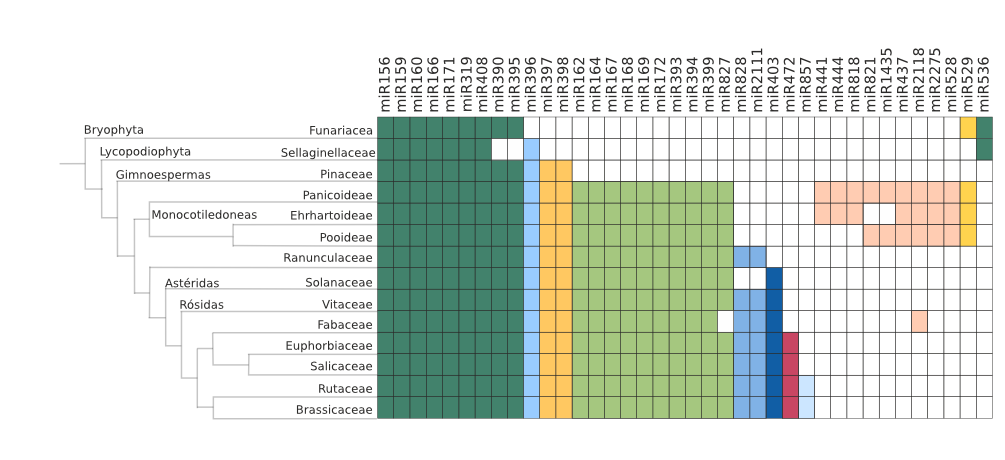
\includegraphics[width=1\textwidth]{img/familias_miRNAs_conservados.png}
	\end{center}
\end{frame}

\begin{frame}{Procesamiento de miARNs en animales}
	\begin{center}
		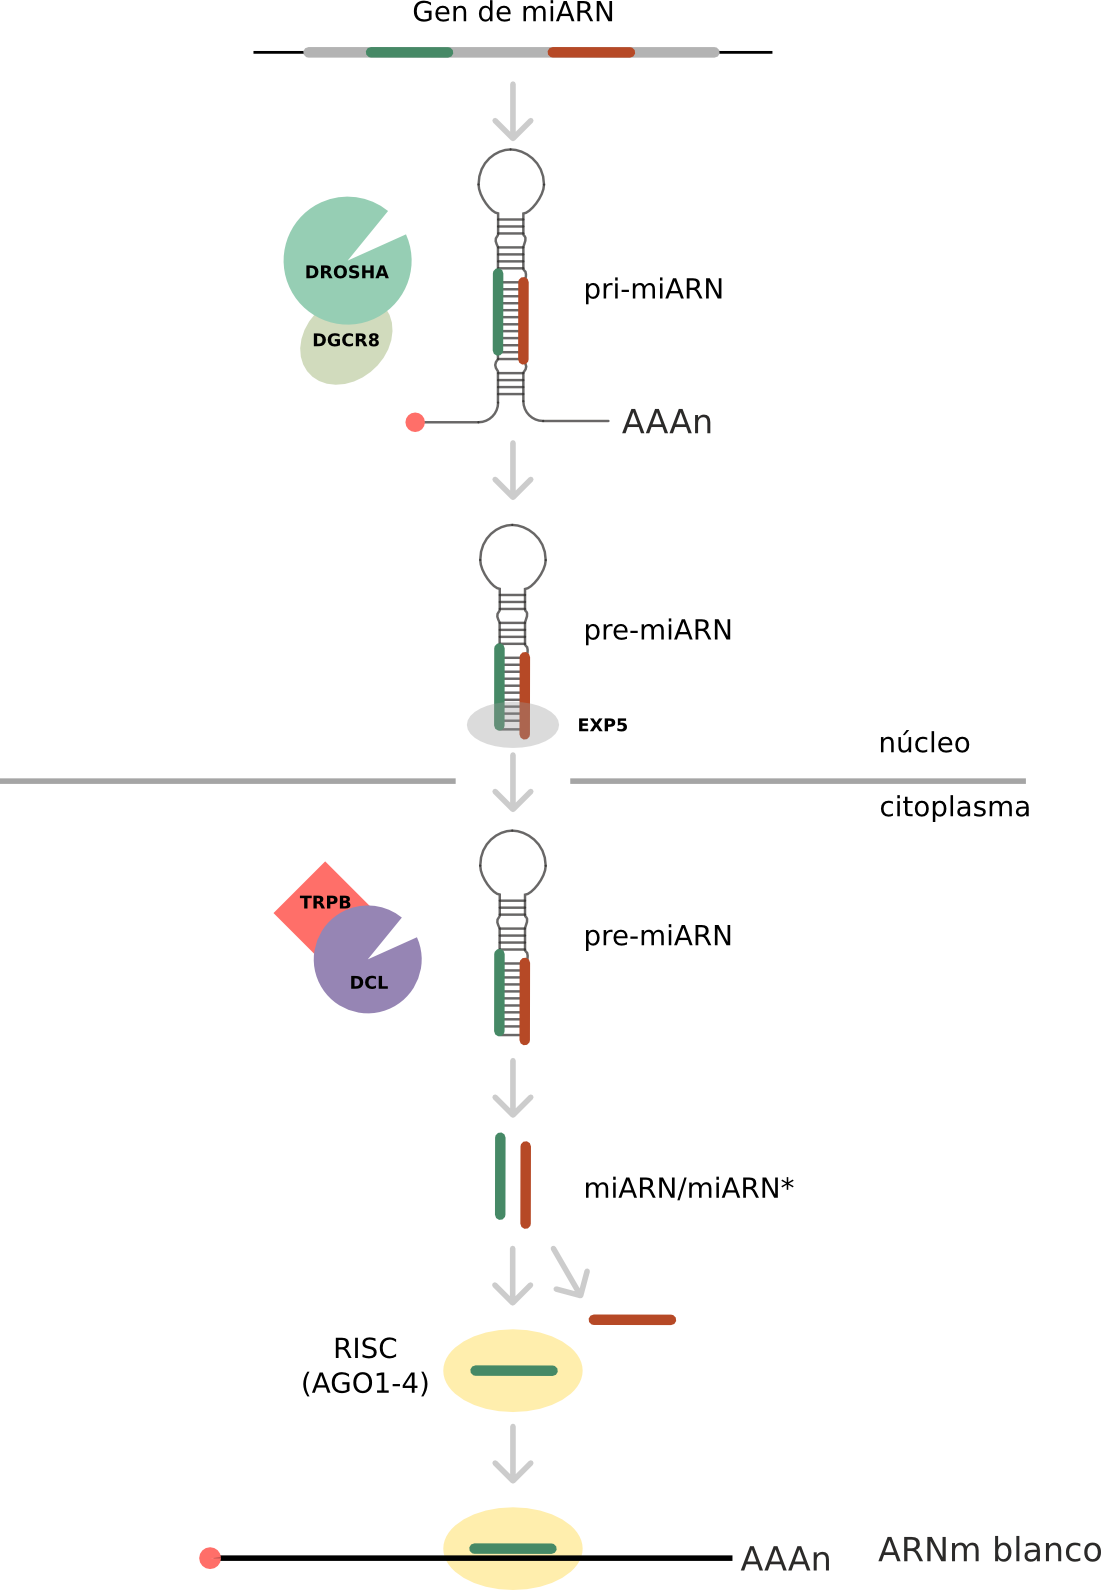
\includegraphics[width=0.5\textwidth]{img/procesamiento_animales.png}
	\end{center}
\end{frame}


\begin{frame}{Biogénesis y actividad de miARNs en plantas}
	\begin{center}
		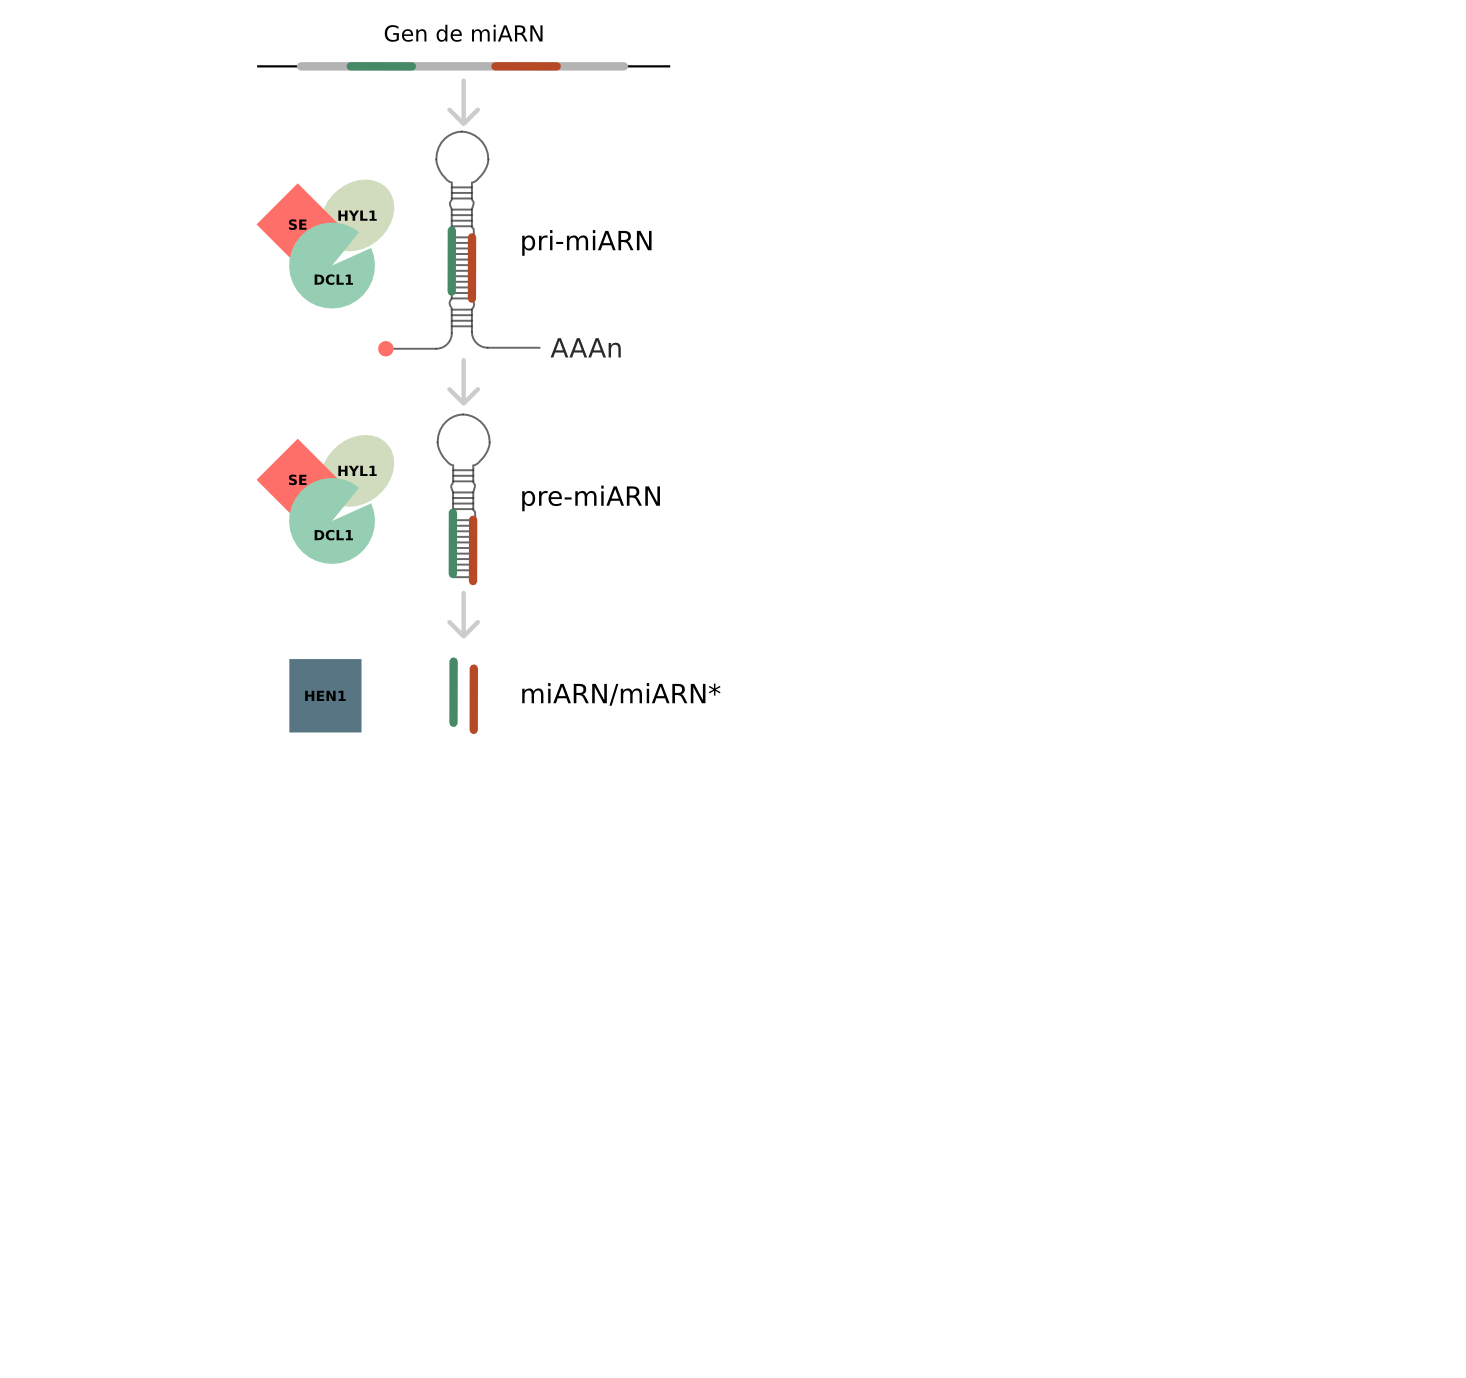
\includegraphics[width=0.7\textwidth]{img/biogenesis_accion_defensa02.png}
	\end{center}
\end{frame}

\begin{frame}{Biogénesis y actividad de miARNs en plantas}
	\begin{center}
		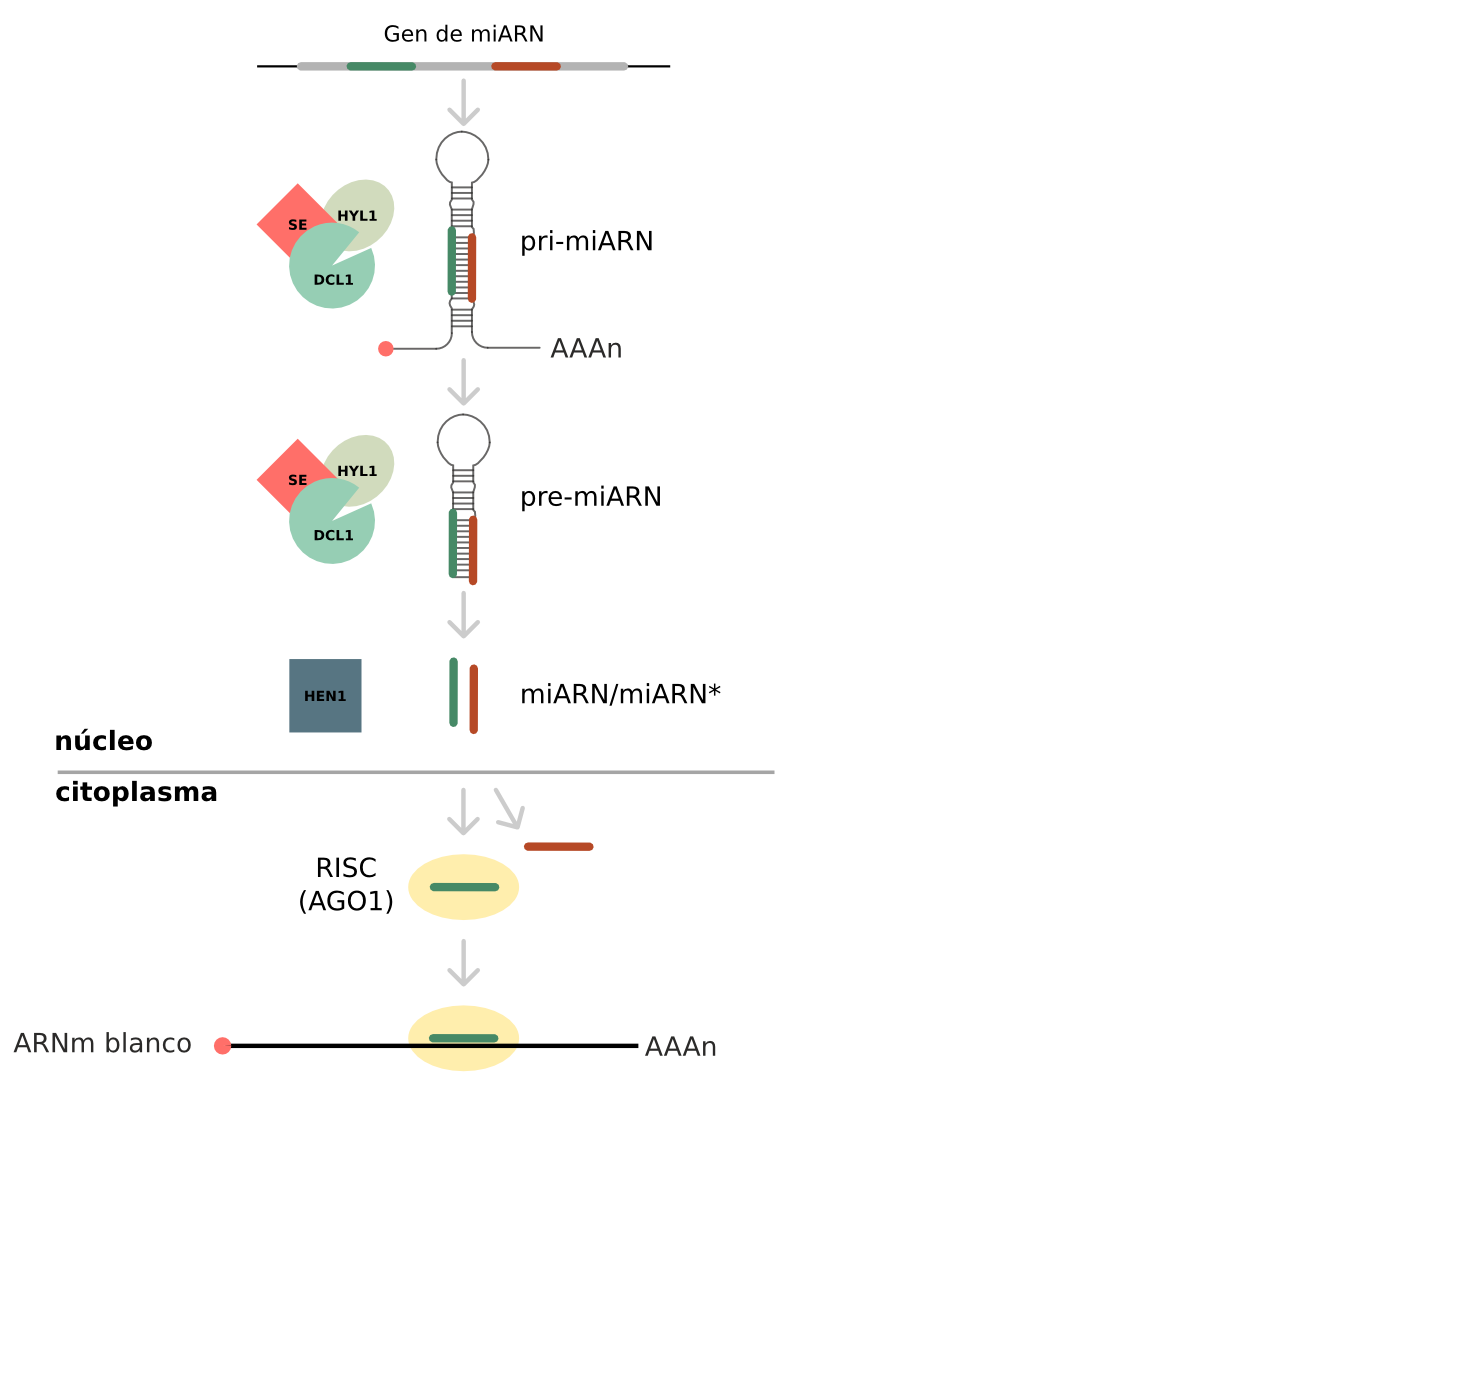
\includegraphics[width=0.7\textwidth]{img/biogenesis_accion_defensa03.png}
	\end{center}
\end{frame}

\begin{frame}{Biogénesis y actividad de miARNs en plantas}
	\begin{center}
		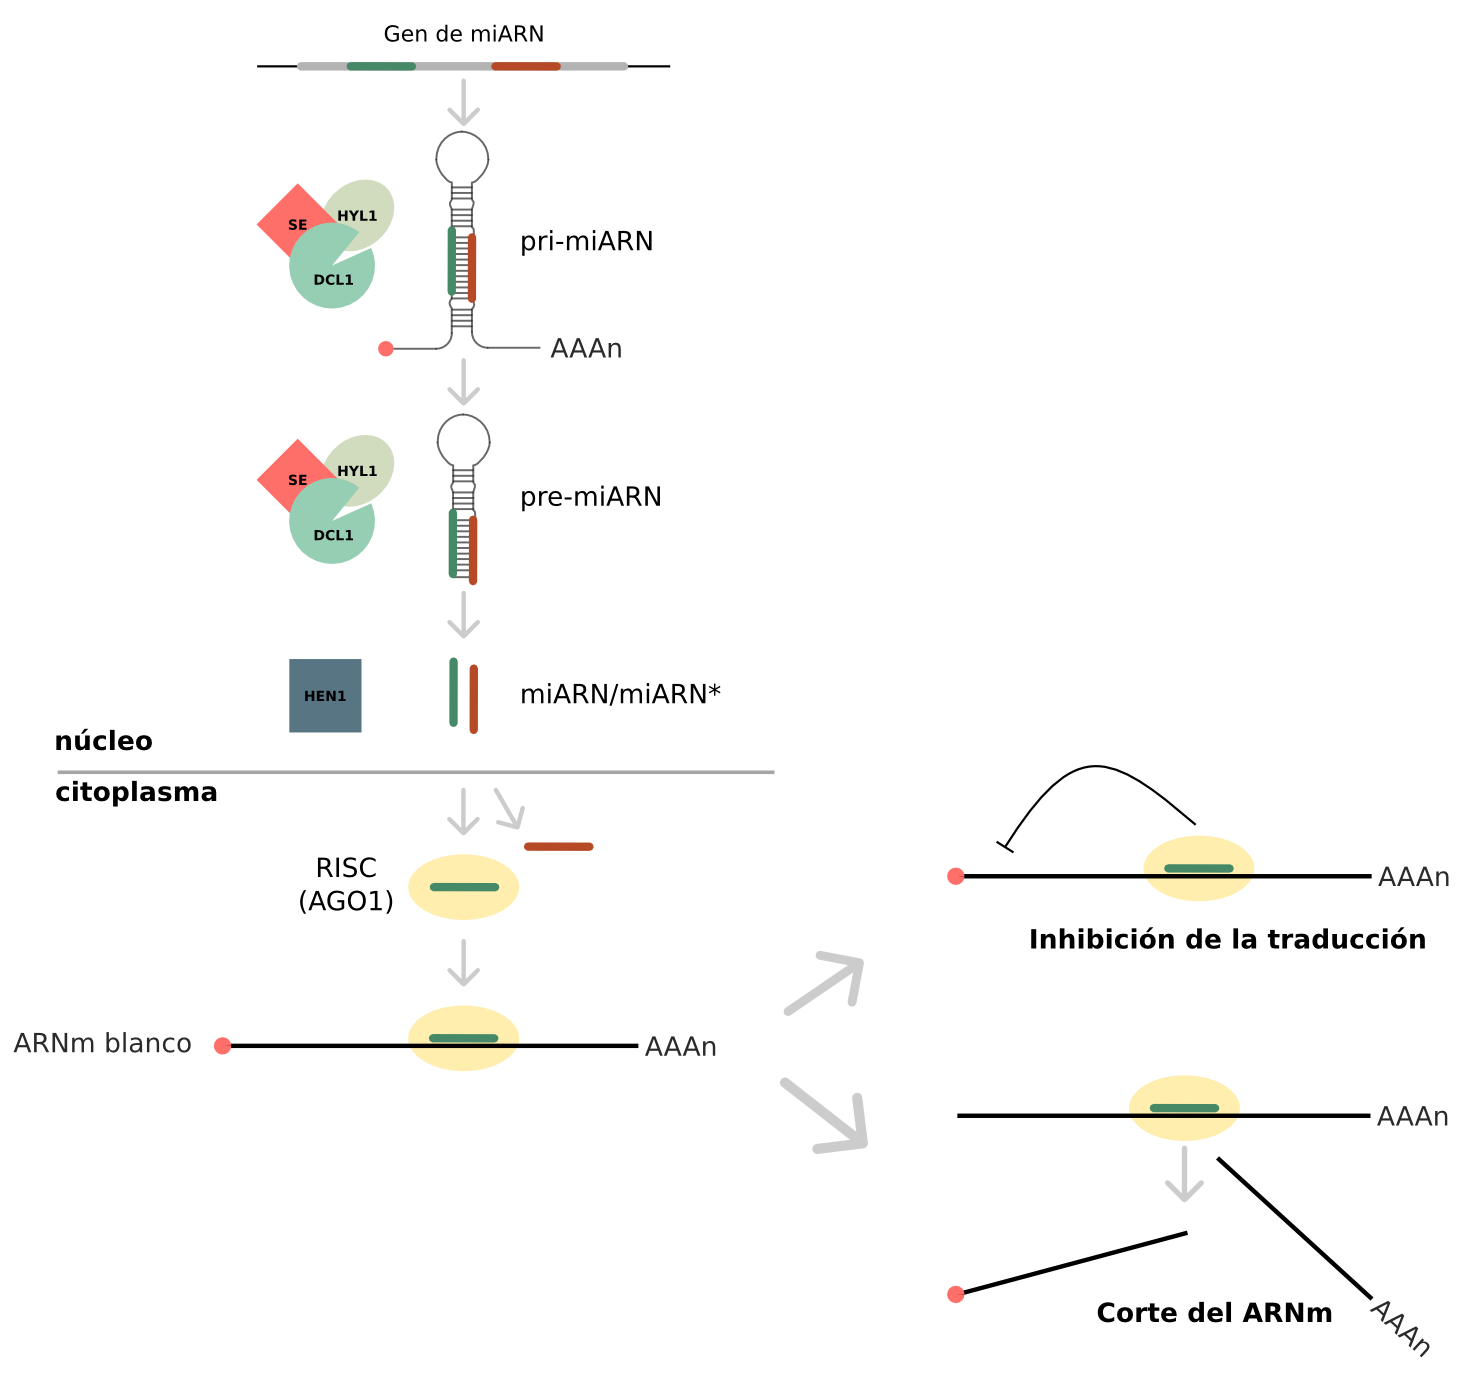
\includegraphics[width=0.7\textwidth]{img/biogenesis_accion_defensa04.png}
	\end{center}
\end{frame}

\begin{frame}{Biogénesis y actividad de miARNs en plantas}
	\begin{center}
		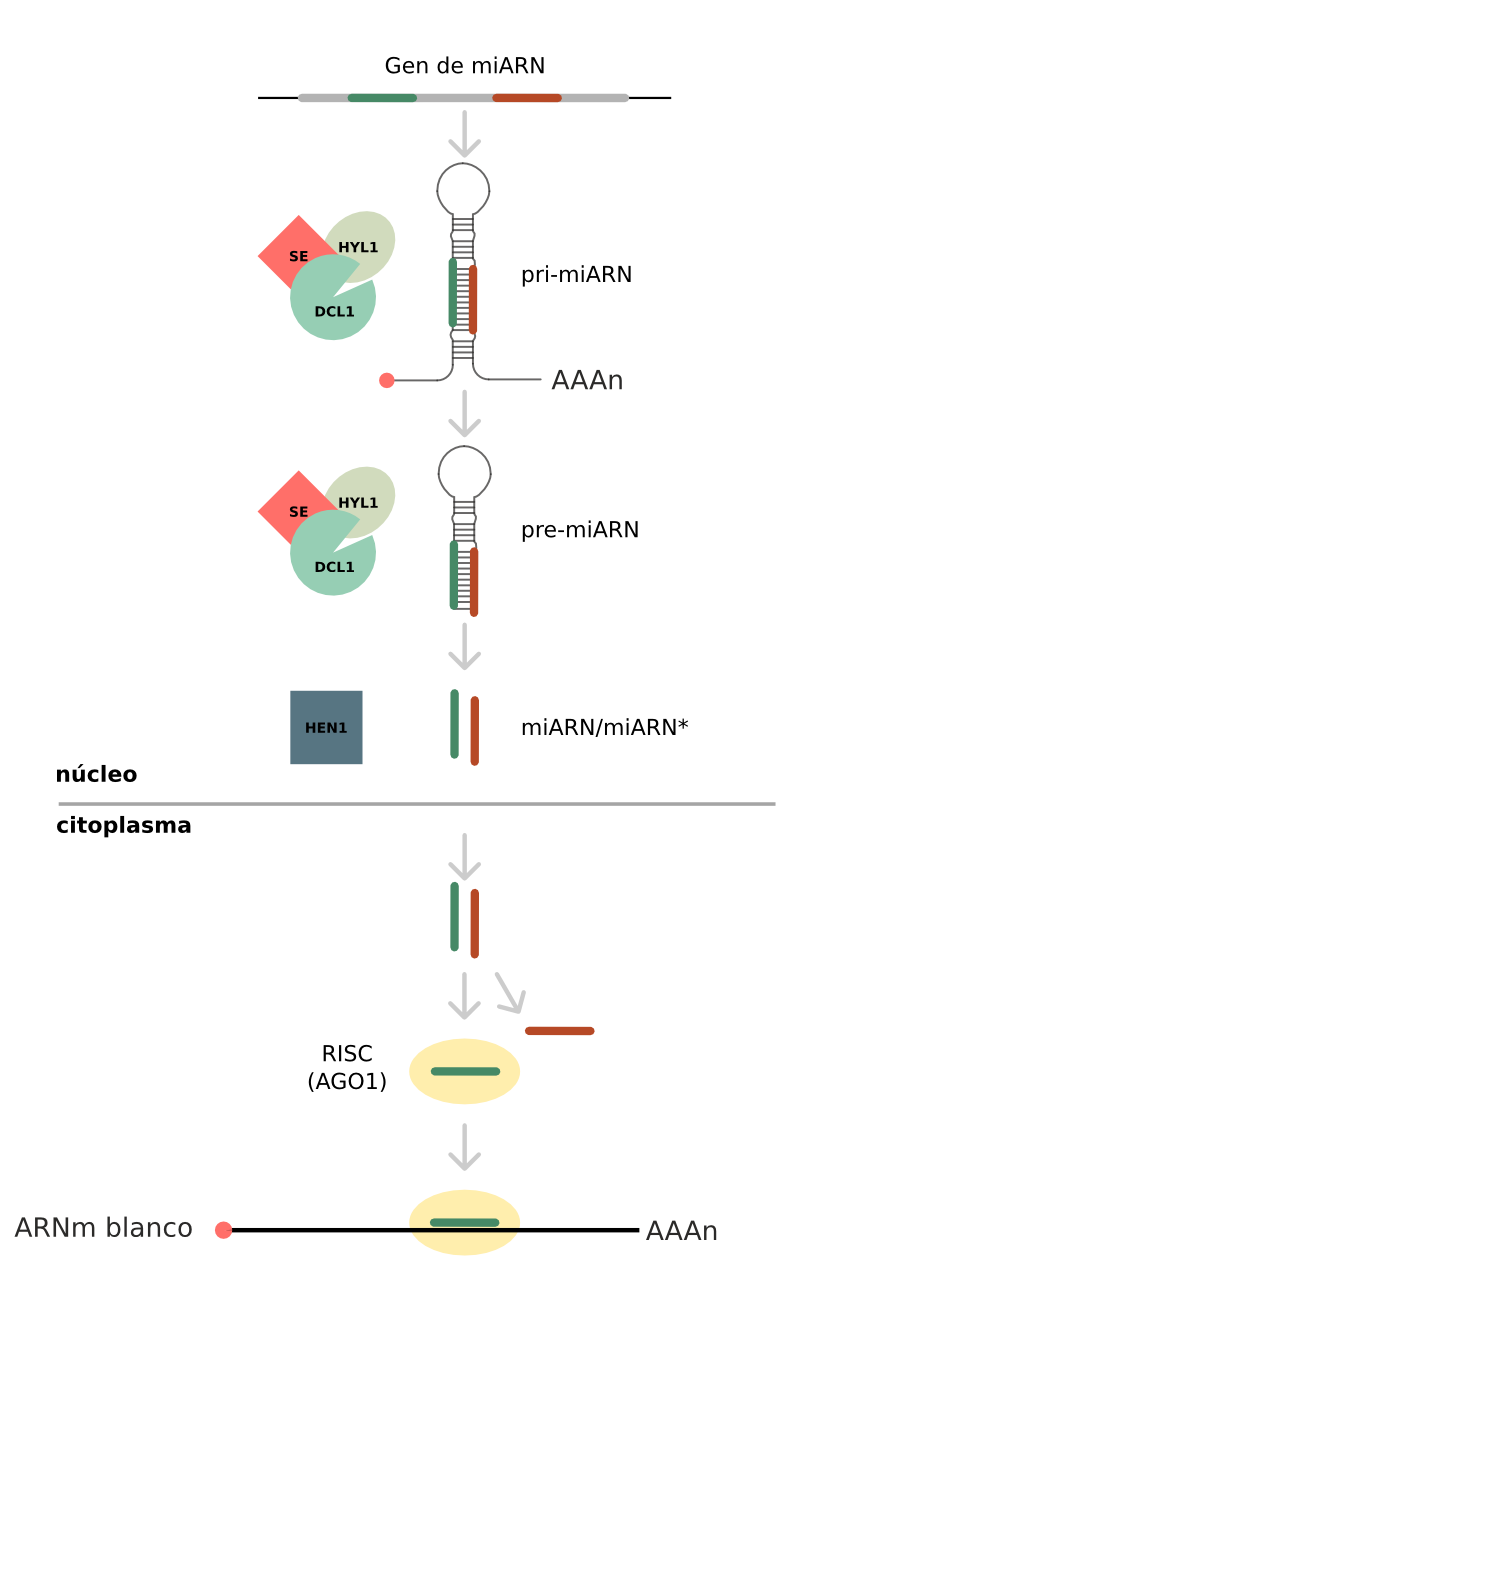
\includegraphics[width=0.7\textwidth]{img/biogenesis_accion_defensa05.png}
	\end{center}
\end{frame}

\begin{frame}{Biogénesis y actividad de miARNs en plantas}
	\begin{center}
		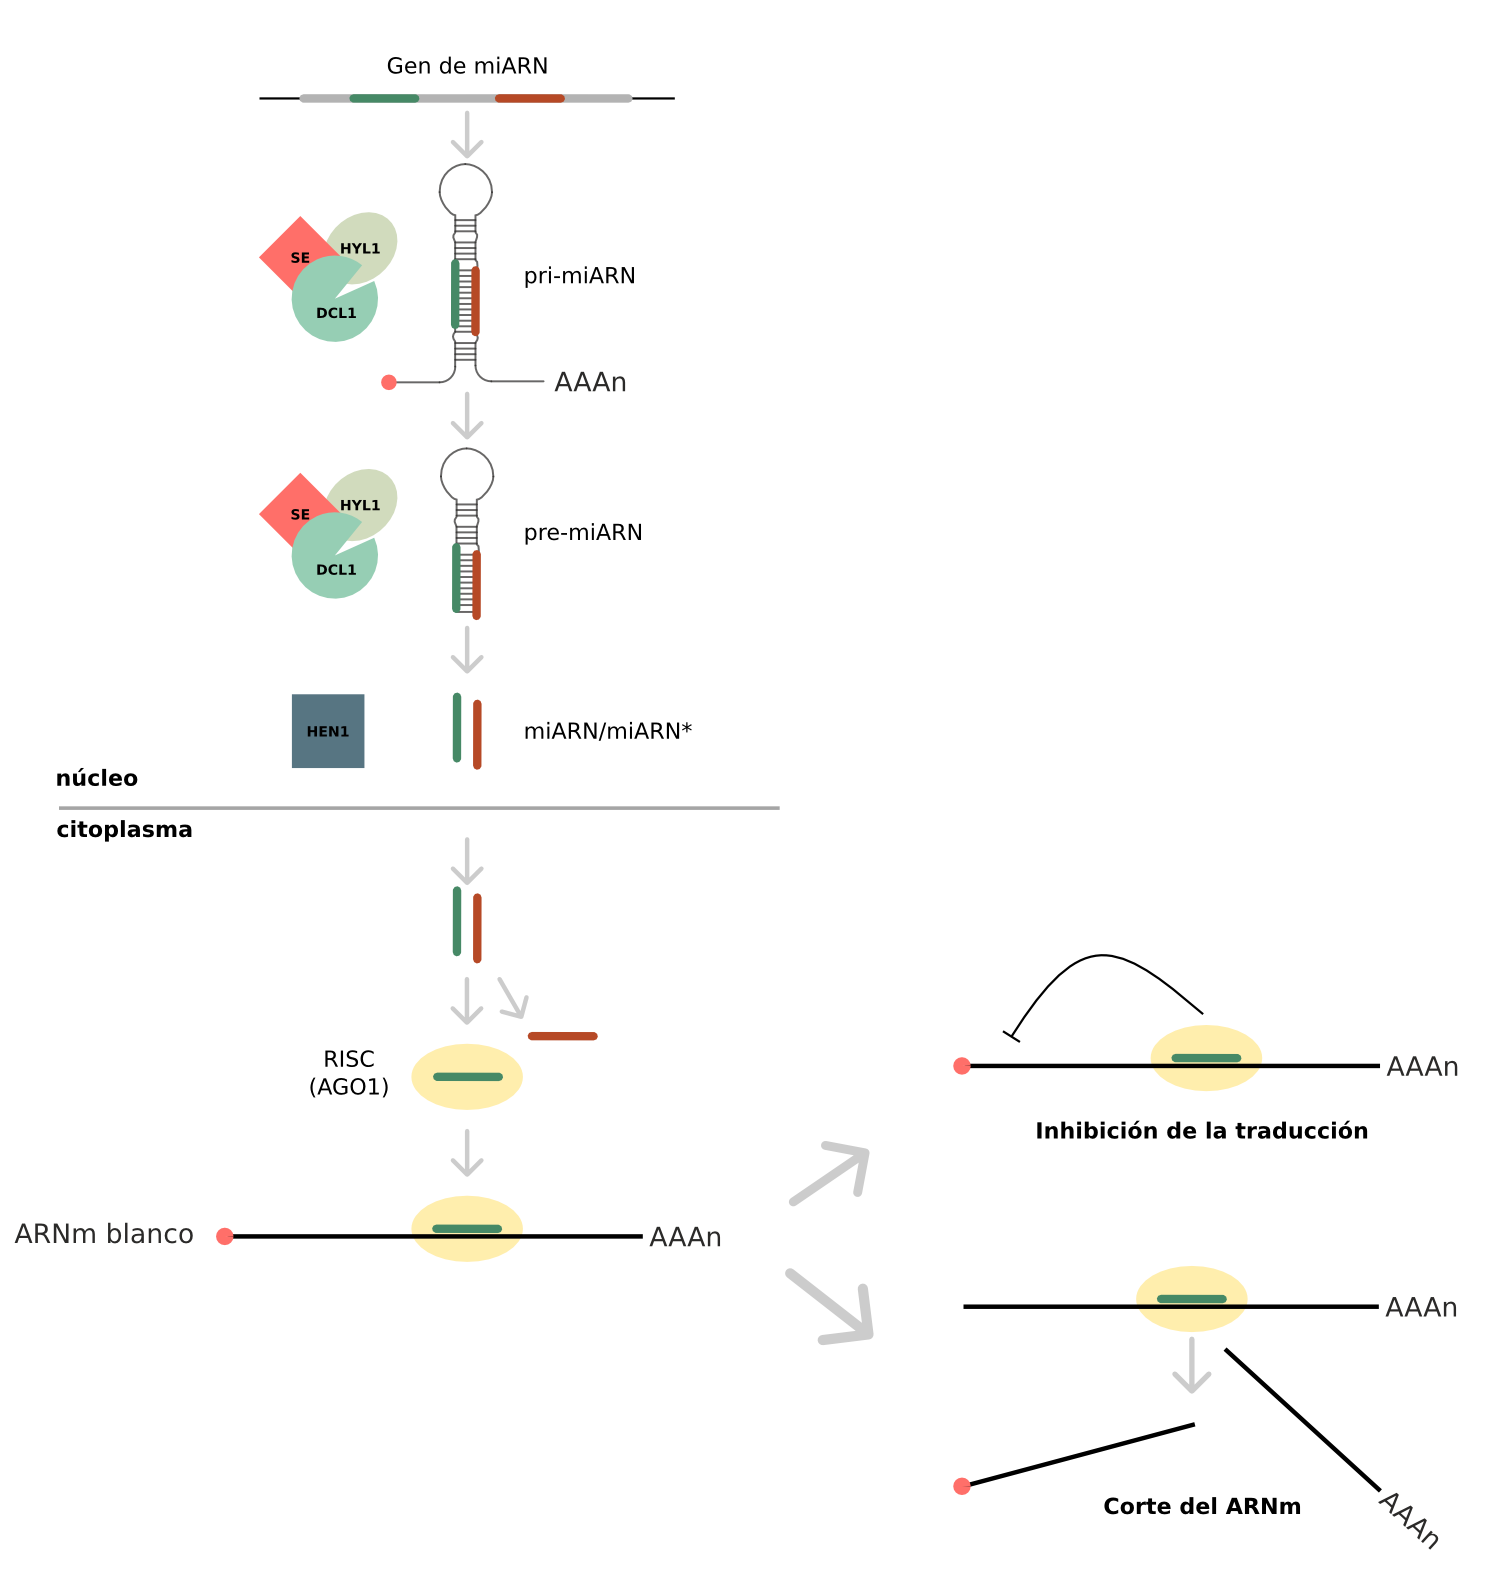
\includegraphics[width=0.7\textwidth]{img/biogenesis_accion_defensa06.png}
	\end{center}
\end{frame}

\begin{frame}{El tamaño de los precursores es muy variado en plantas}
	\begin{center}
		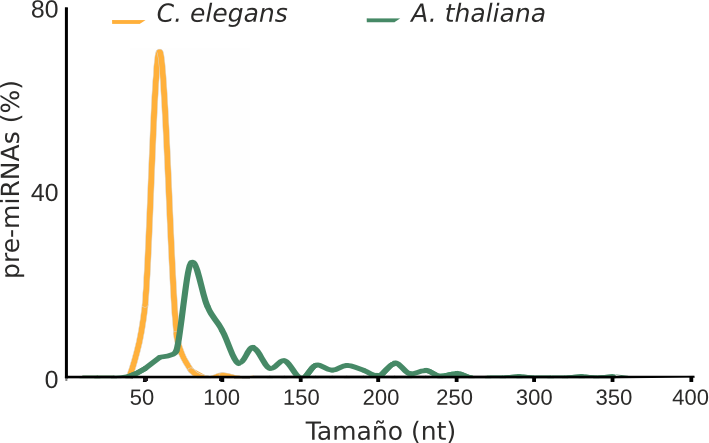
\includegraphics[width=0.5\textwidth]{img/distribucion_precursores.png}
	\end{center}
\end{frame}

\begin{frame}{Estructuras secundarias de precursores de miARNs}
	\begin{center}
		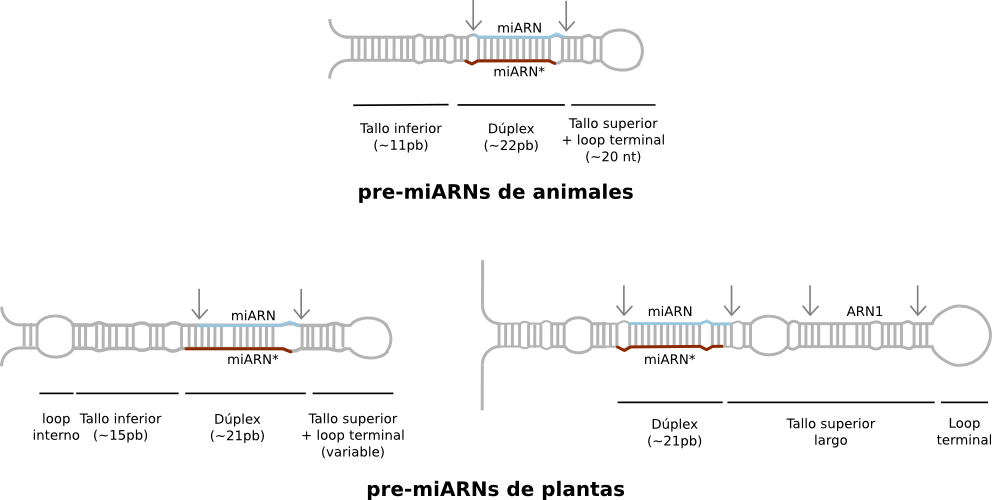
\includegraphics[width=1\textwidth]{img/ss_precursores.png}
	\end{center}
\end{frame}

\begin{frame}{Regulación de la expresión génica por miARNs}
En animales existe un gran número de genes blanco mediado por miARNs y un ARNm puede estar regulado por varios miARNs, en cambio los miARNs en plantas regulan un número limitado de genes blanco.
    \begin{itemize}
        \item<2-> Regulación por corte del ARN blanco.
        \begin{itemize}
            \item Es el mecanismo más común en plantas.
            \item El corte ocurre entre las posiciones 10 y 11 desde el extremo 5’ del miARN.
        \end{itemize}
        \item<3-> Regulación de la traducción por miARNs.
        \begin{itemize}
            \item Inhibición de la traducción del ARNm blanco por el miARN explica la represión de la expresión de los blancos de miARNs en animales.
            \item Otras veces los miARNs de animales disminuyen la vida media de los transcriptos a los que se unen.
        \end{itemize}

    \end{itemize}
\end{frame}

\begin{frame}{Predicción de genes blanco de miARNs}
	\begin{center}
		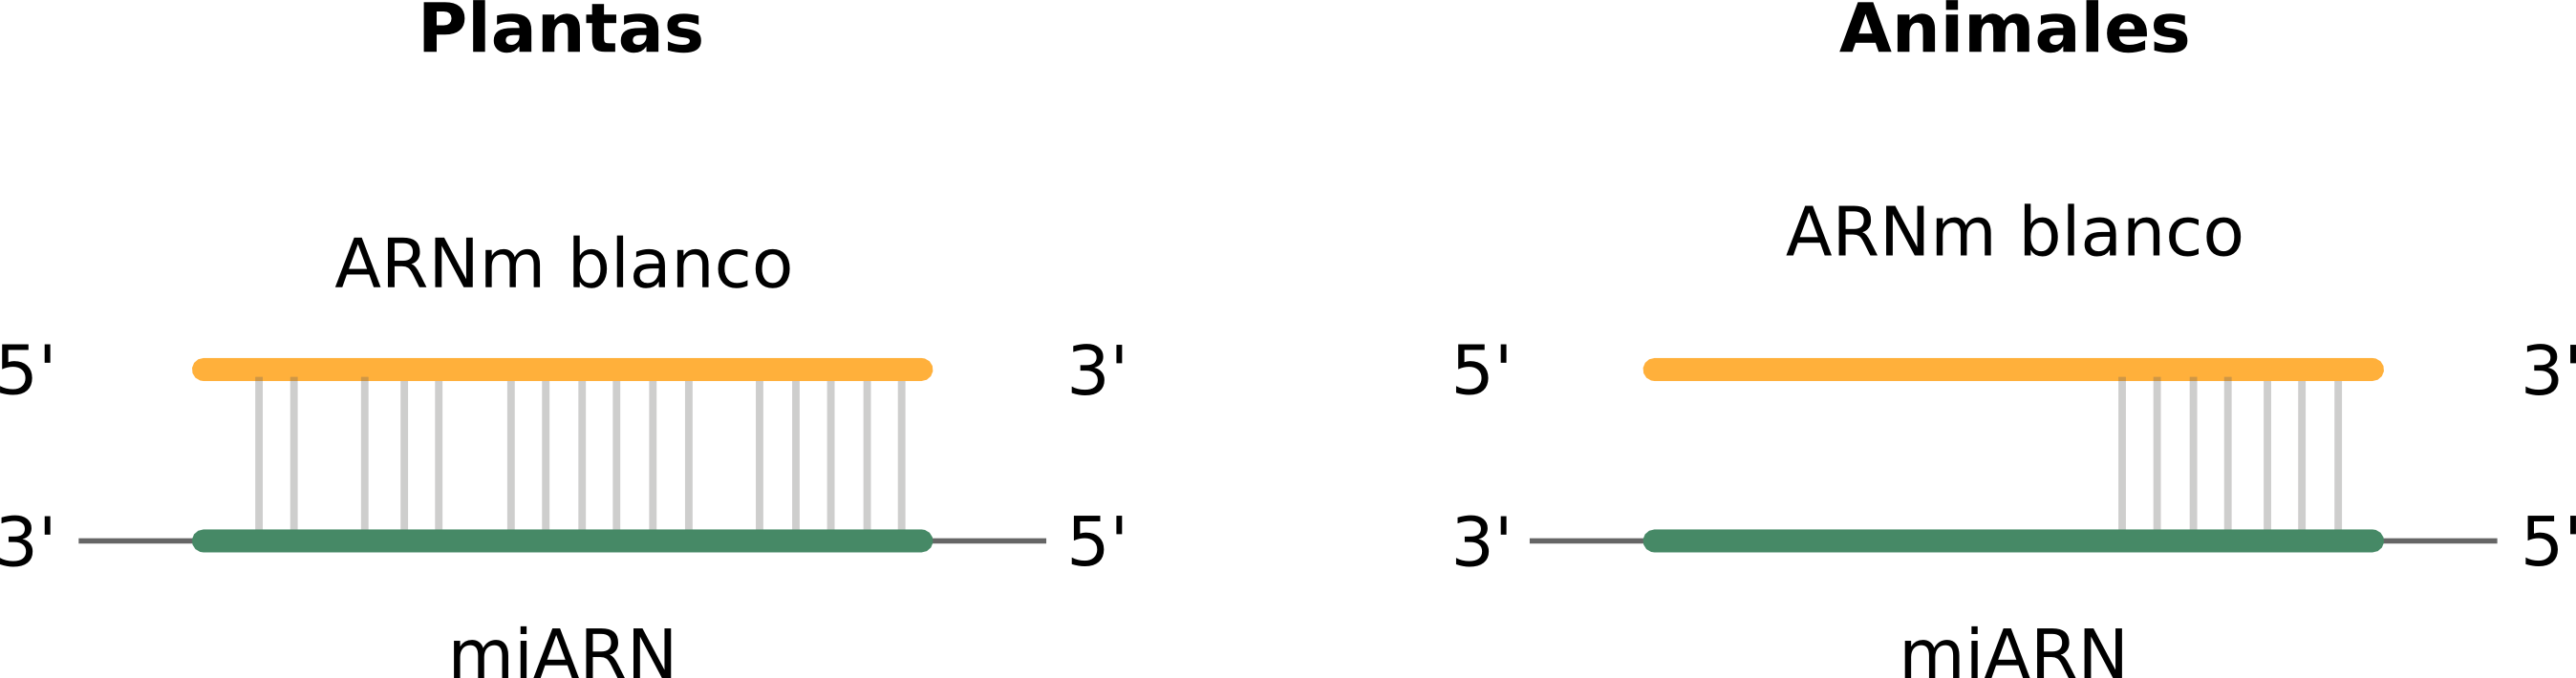
\includegraphics[width=1\textwidth]{img/interaccion_miRNA_target.png}
	\end{center}
\end{frame}


\section{Objetivos}

\begin{frame}{Objetivos}
    Diseñar estrategias computacionales para:
    \setbeamercovered{transparent=25}
	\begin{itemize}[<+->]
        \item identificar redes regulatorias de miARNs en plantas.
        \item comprender la biogénesis de los miARNs en plantas.
	\end{itemize}
\end{frame}

\begin{frame}{Objetivos específicos}
    \setbeamercovered{transparent=25}
		\pause
		\begin{itemize}
            \item<-2> Diseñar una estrategia para la identificación de genes blancos regulados por miARNs.
			\item<-1> Caracterizar precursores de miARNs en distintas especies que tengan mecanismos de procesamiento distintos.
			\item<-1> Caracterizar la relación entre la evolución de los precursores de miARNs en plantas y los mecanismos de procesamiento determinados previamente.
        \end{itemize}
\end{frame}


\section{Resultados}

\subsection{Resultados 1}

%~ Aplicaciones bioinformáticas para el estudio de interacciones miARN-gen blanco

%~ La identificación de genes blancos regulados por miARNs en plantas es muy importante para poder conocer el rol de los miARNs

\begin{frame}{Problemáticas y dificultades a la hora de identificar genes regulados por miARNs}
	\begin{itemize}
		\item Estrategias computacionales donde tienen en cuenta la complementariedad con sus mensajeros blanco.
        \item Uno de los mayores desafíos es predecir los genes regulados por estos ARN pequeños con una baja frecuencia de predicciones falsas.
	\end{itemize}
\end{frame}

\begin{frame}{Conservación y divergencia de miARNs en distintas especies}
	\begin{center}
		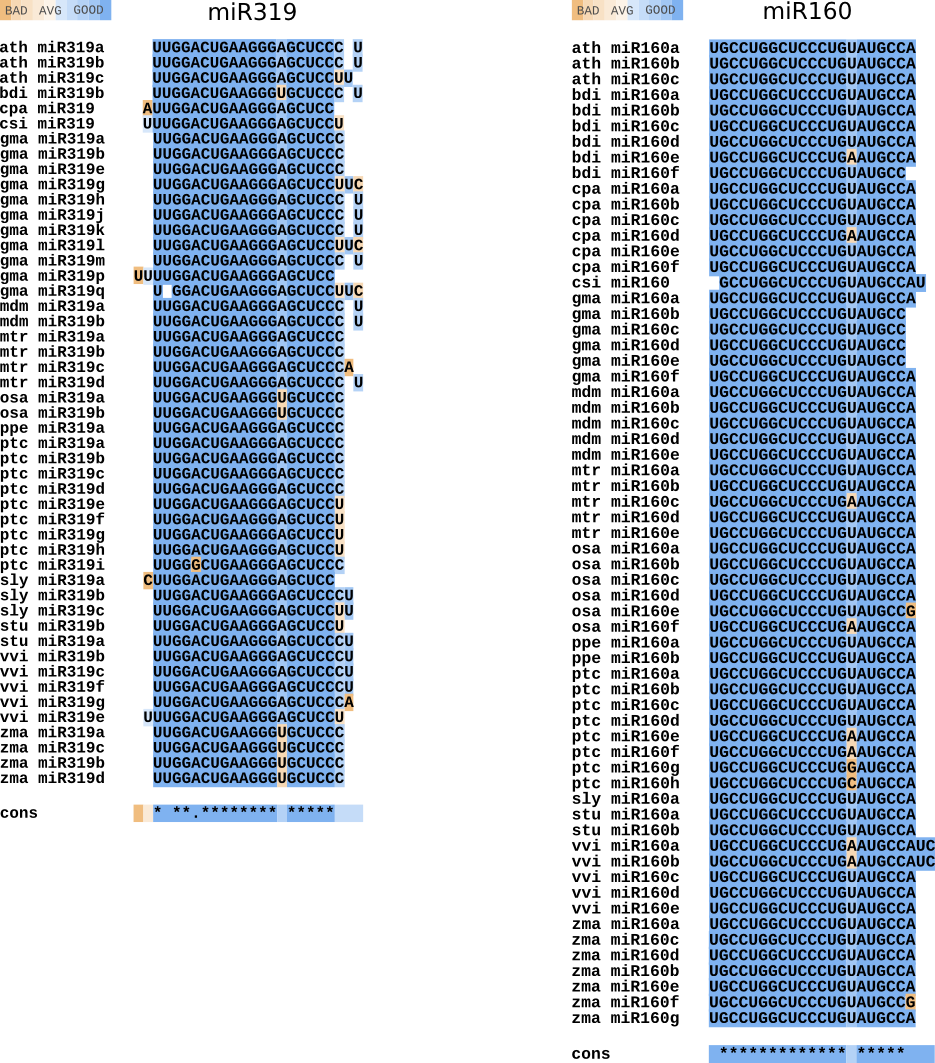
\includegraphics[width=0.6\textwidth]{img/variabilidad_maduro.png}
	\end{center}
\end{frame}

\begin{frame}{Esquema de la estrategia para la identificación de nuevos genes blancos}
	\begin{center}
		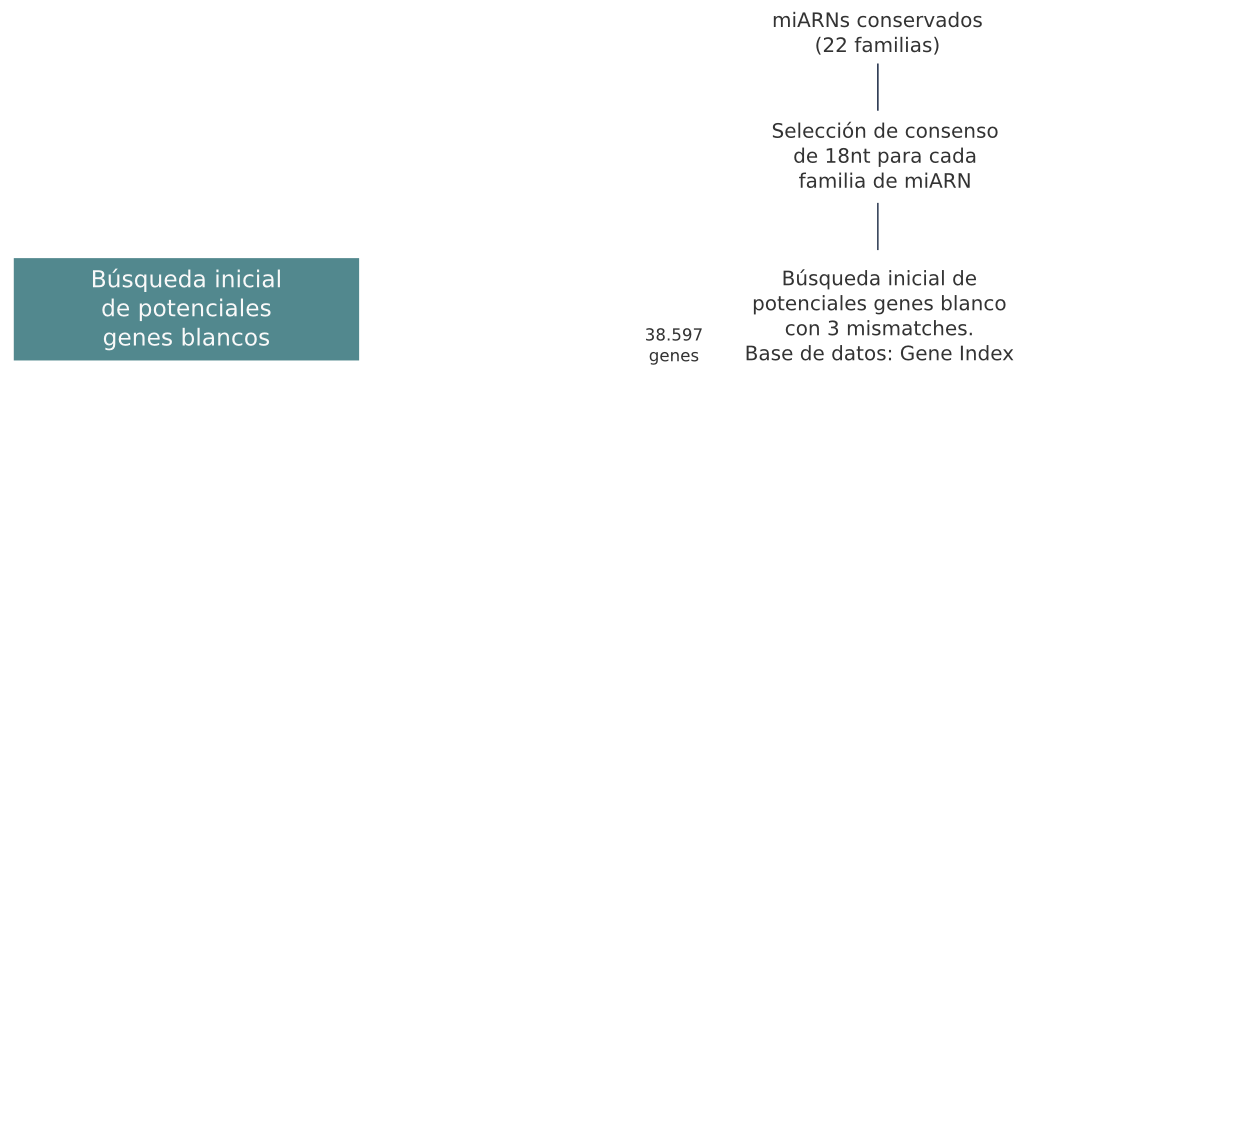
\includegraphics[width=0.7\textwidth]{img/NAR_fig01_01.png}
	\end{center}
\end{frame}

\begin{frame}{Esquema de la estrategia para la identificación de nuevos genes blancos}
	\begin{center}
		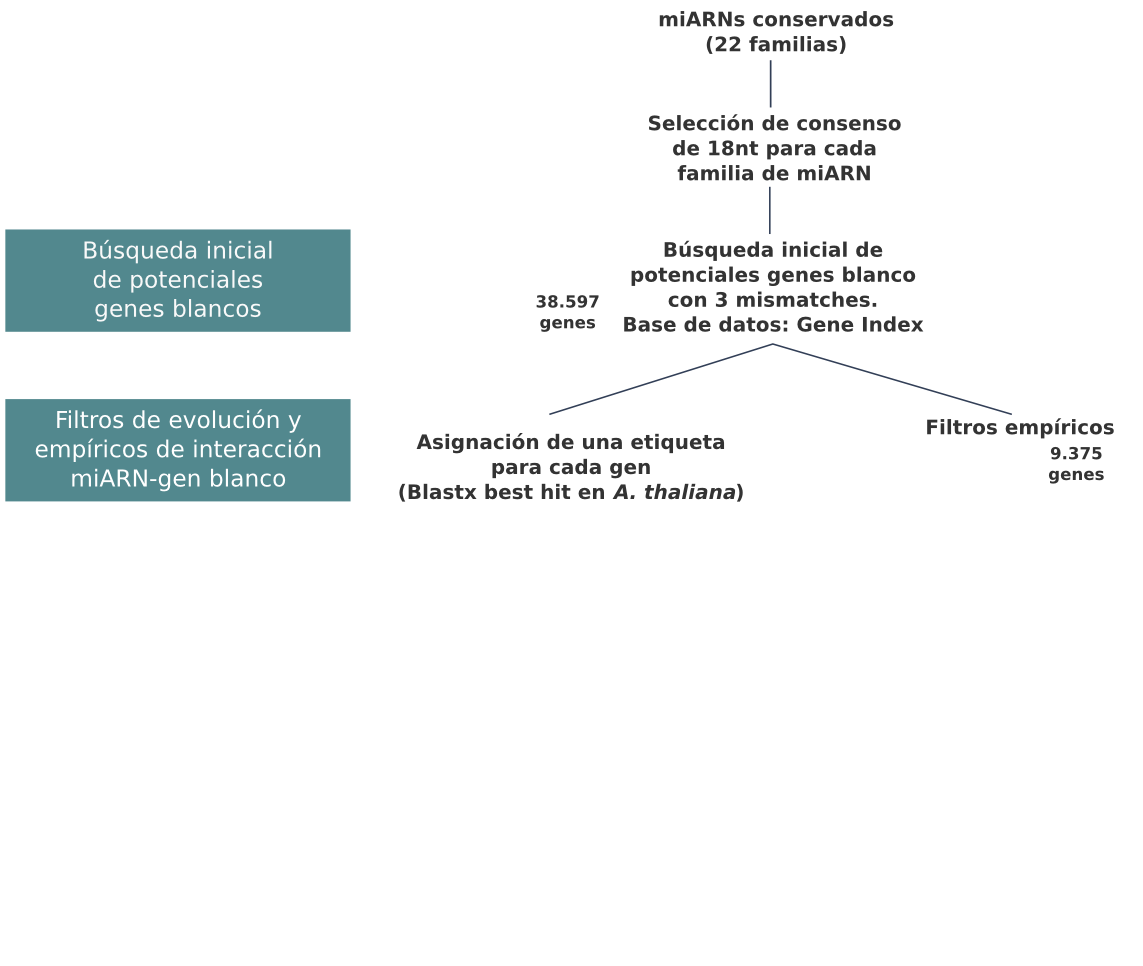
\includegraphics[width=0.7\textwidth]{img/NAR_fig01_02.png}
	\end{center}
\end{frame}


\begin{frame}{Esquema de la estrategia para la identificación de nuevos genes blancos}
	\begin{center}
		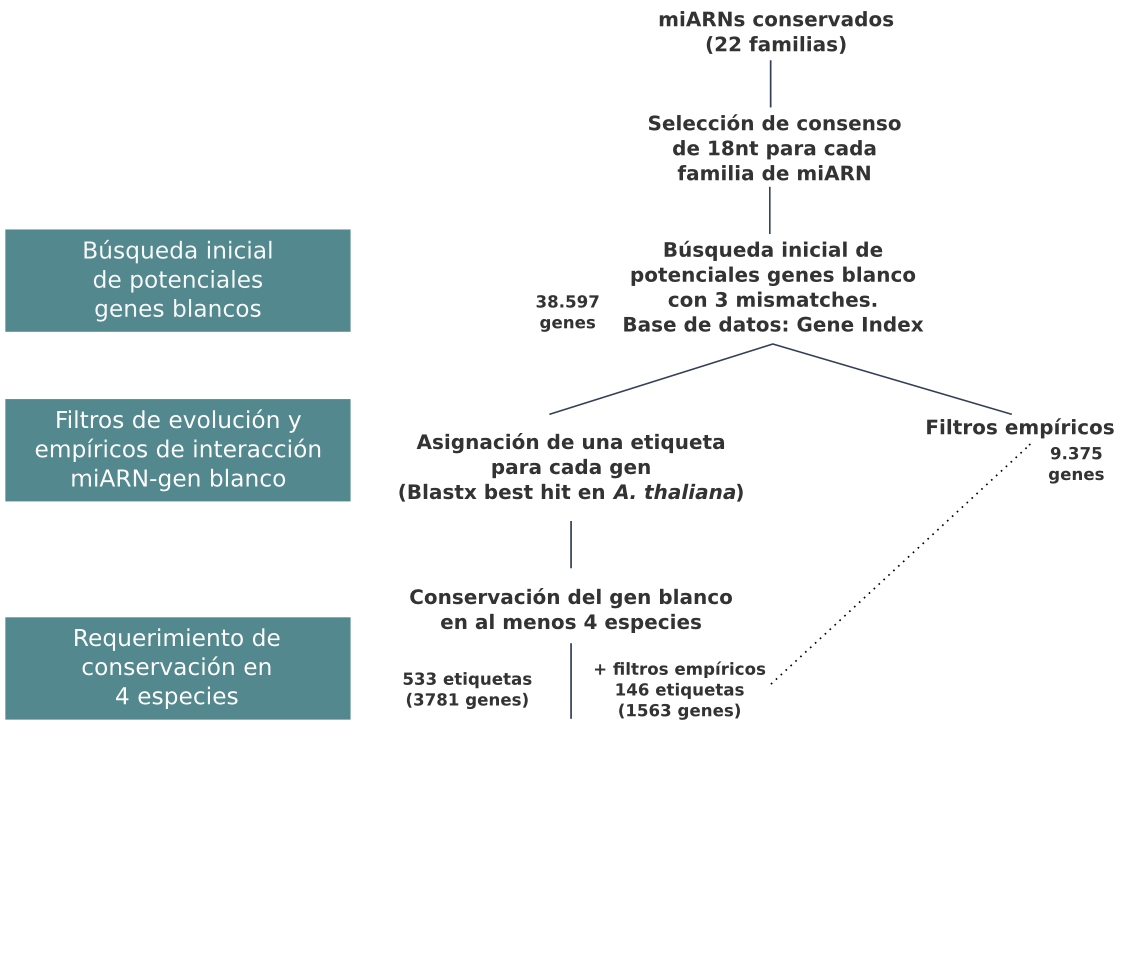
\includegraphics[width=0.7\textwidth]{img/NAR_fig01_03.png}
	\end{center}
\end{frame}


\begin{frame}{Esquema de la estrategia para la identificación de nuevos genes blancos}
	\begin{center}
		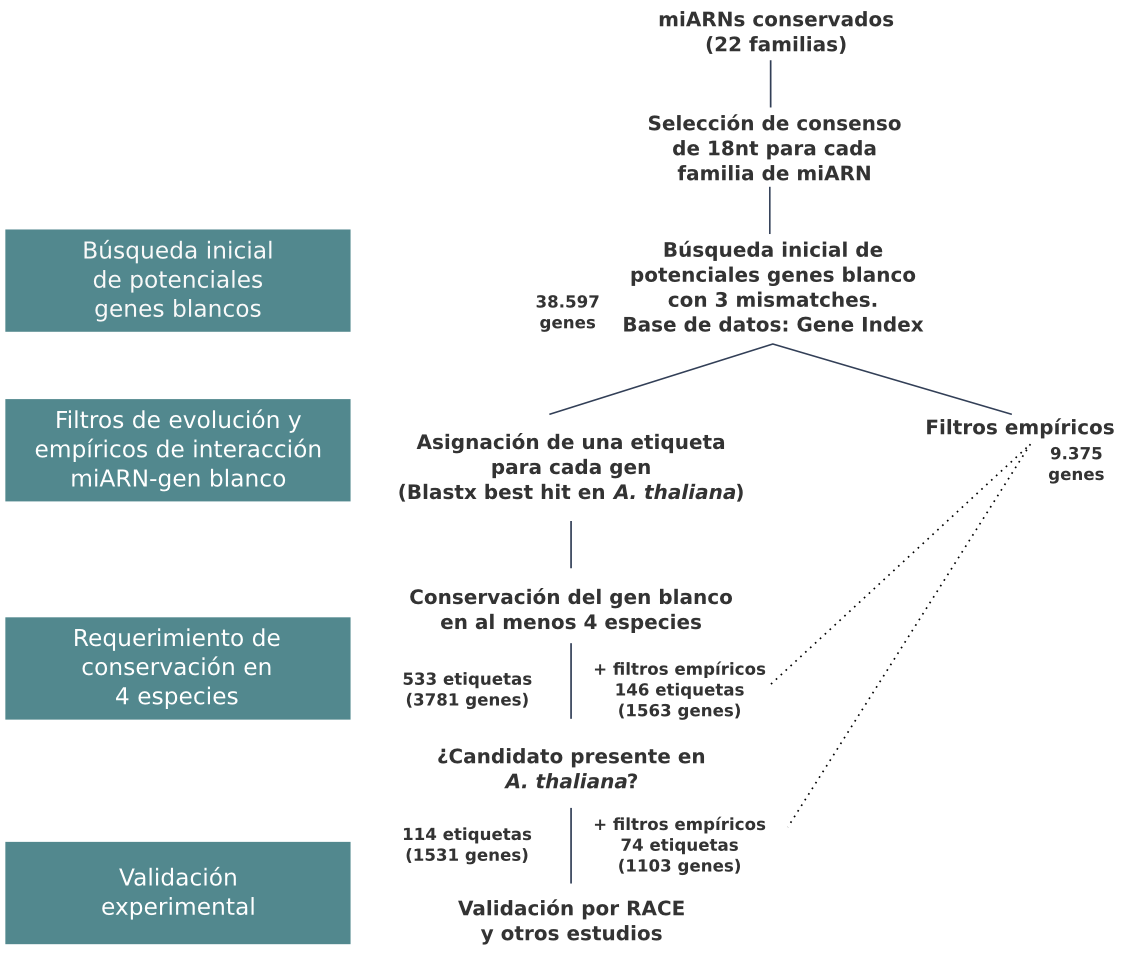
\includegraphics[width=0.7\textwidth]{img/NAR_fig01_04.png}
	\end{center}
\end{frame}

\begin{frame}{Conservación de la interacción en distintas especies}
	\begin{center}
		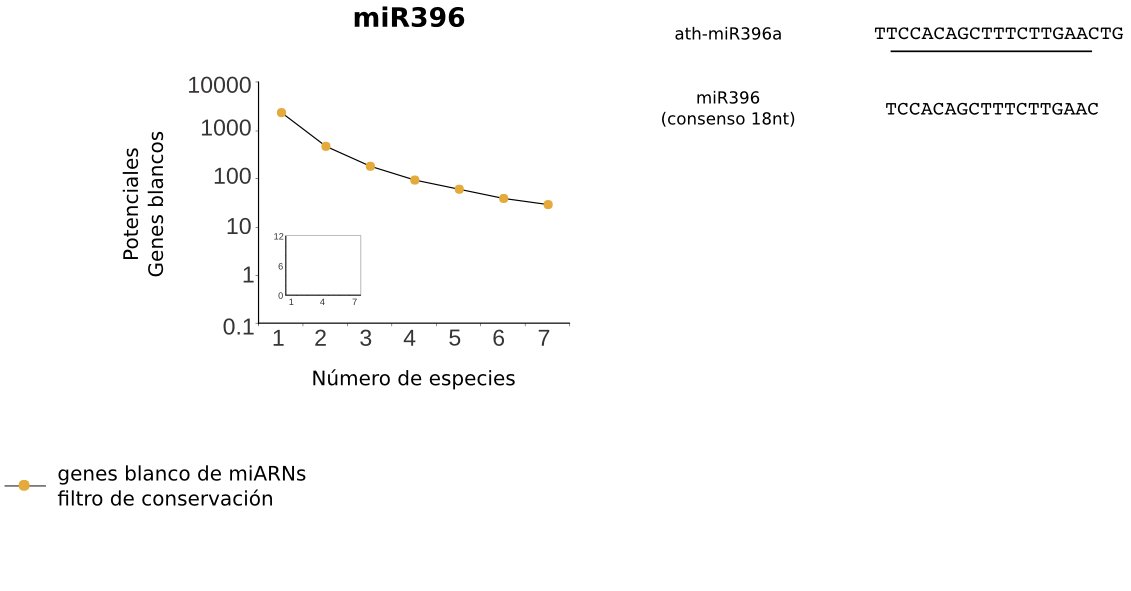
\includegraphics[width=1\textwidth]{img/NAR_fig2_01.png}
	\end{center}
\end{frame}


\begin{frame}{miARN consenso de 18 nt}
	\begin{center}
		
\includegraphics[width=0.5\textwidth]{img/shuffle_01.png}
	\end{center}
\end{frame}

\begin{frame}{Control: miARN al azar}
	\begin{center}
		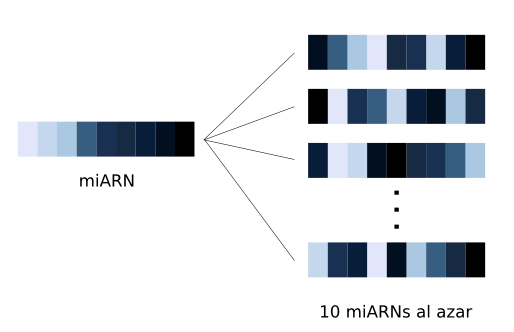
\includegraphics[width=0.5\textwidth]{img/shuffle_02.png}
	\end{center}
\end{frame}

\begin{frame}{La relación señal/ruido incrementa al aumentar el número de especies}
	\begin{center}
		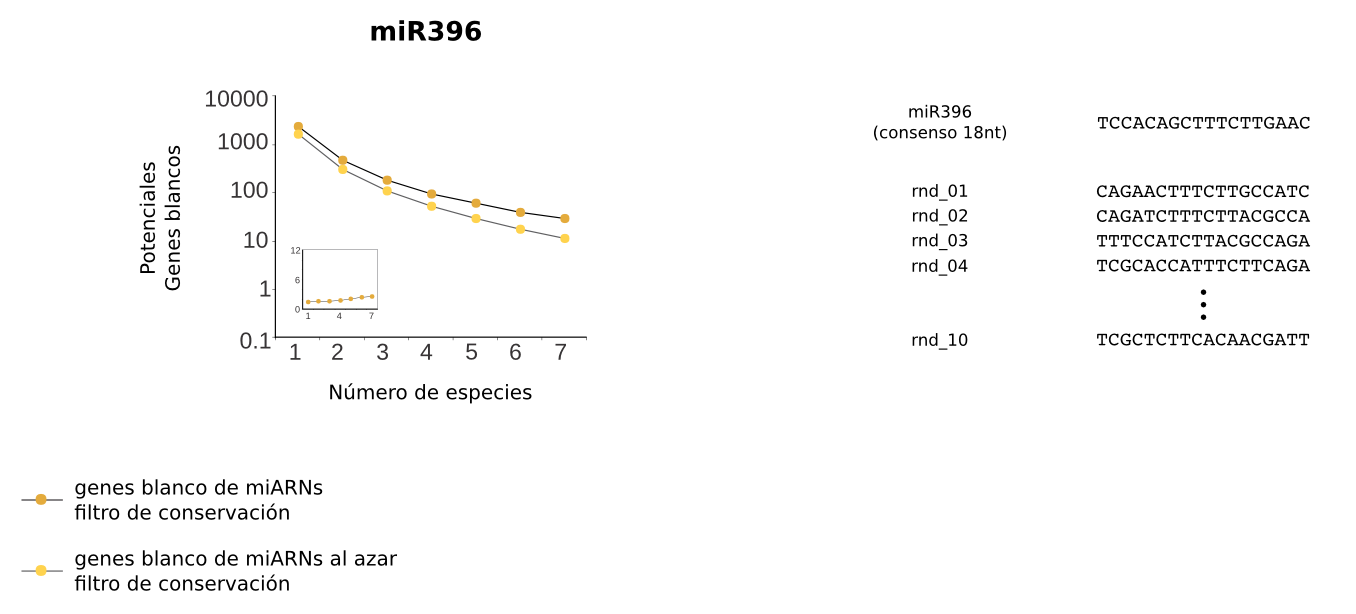
\includegraphics[width=1\textwidth]{img/NAR_fig2_02.png}
	\end{center}
\end{frame}


\begin{frame}{Parámetros empíricos deducidos de interacciones miARN-gen blanco validadas experimentalmente.}
	\begin{center}
		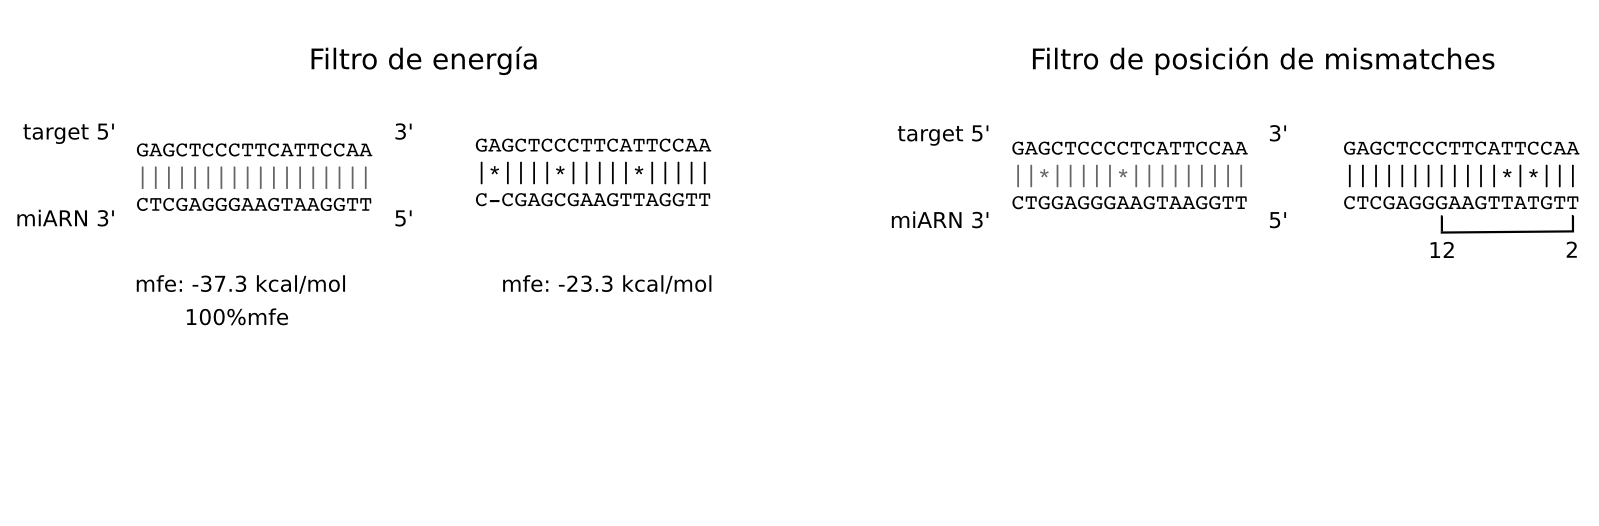
\includegraphics[width=1\textwidth]{img/filtros_empiricos_01.png}
	\end{center}
\end{frame}

\begin{frame}{Parámetros empíricos deducidos de interacciones miARN-gen blanco validadas experimentalmente. Filtros aplicados en nuestra estrategia.}
	\begin{center}
		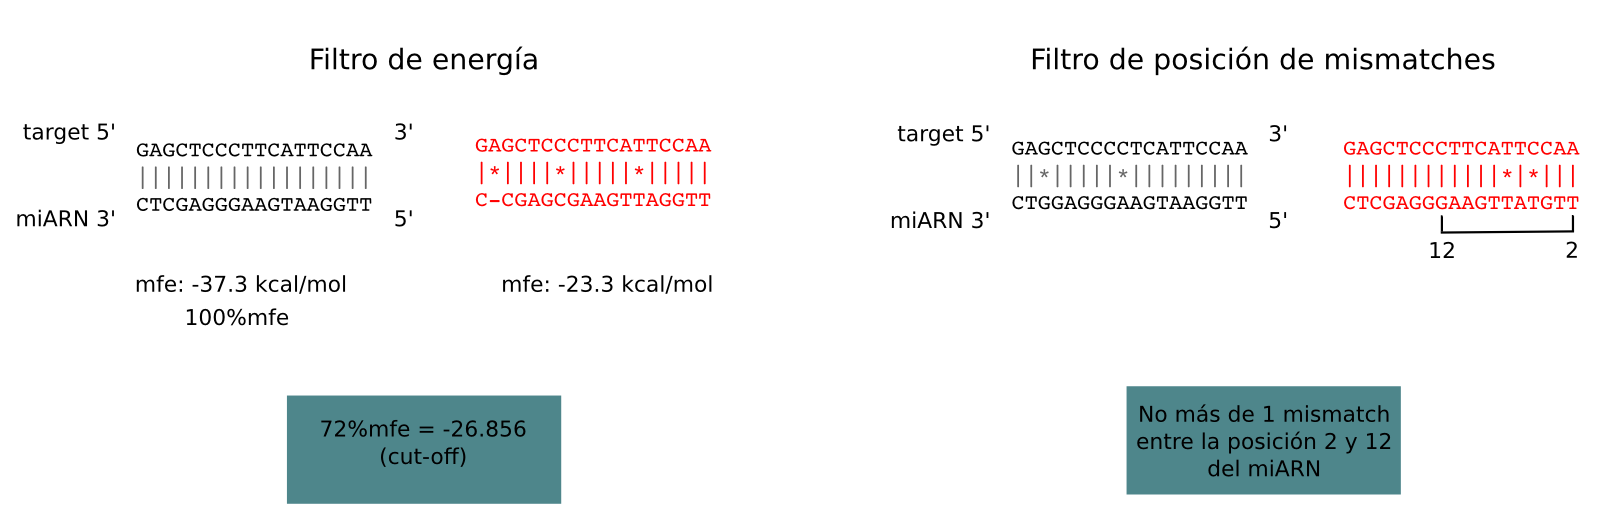
\includegraphics[width=1\textwidth]{img/filtros_empiricos_02.png}
	\end{center}
\end{frame}


\begin{frame}{Slección de candidatos teniendo en cuenta los filtros empíricos}
	\begin{center}
		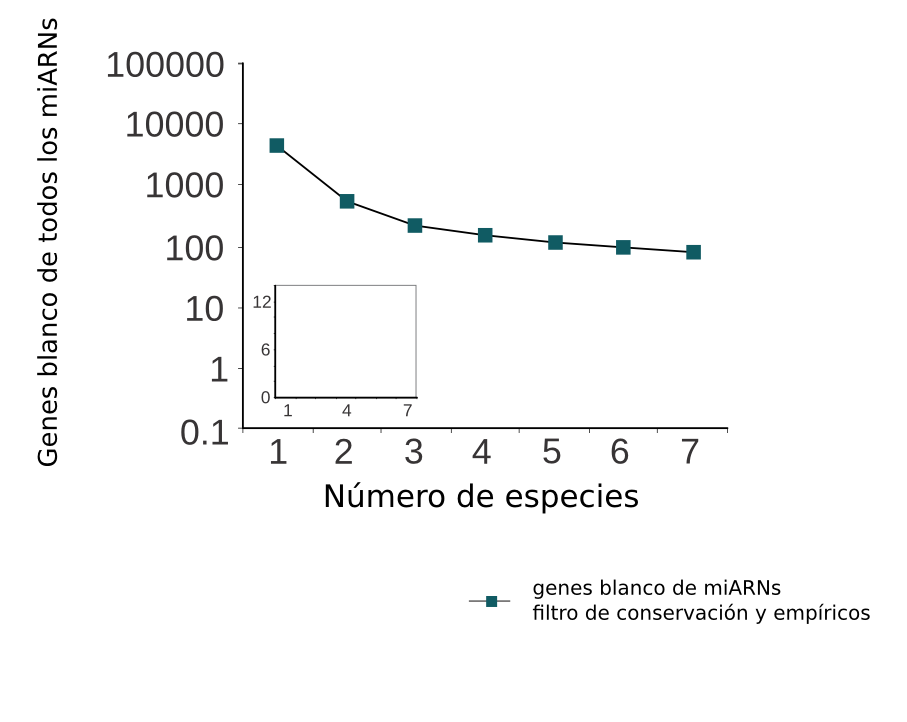
\includegraphics[width=1\textwidth]{img/NAR_fig2_03.png}
	\end{center}
\end{frame}

\begin{frame}{Al aplicar filtros empíricos y de conservación la relación señal/ruido aumenta}
	\begin{center}
		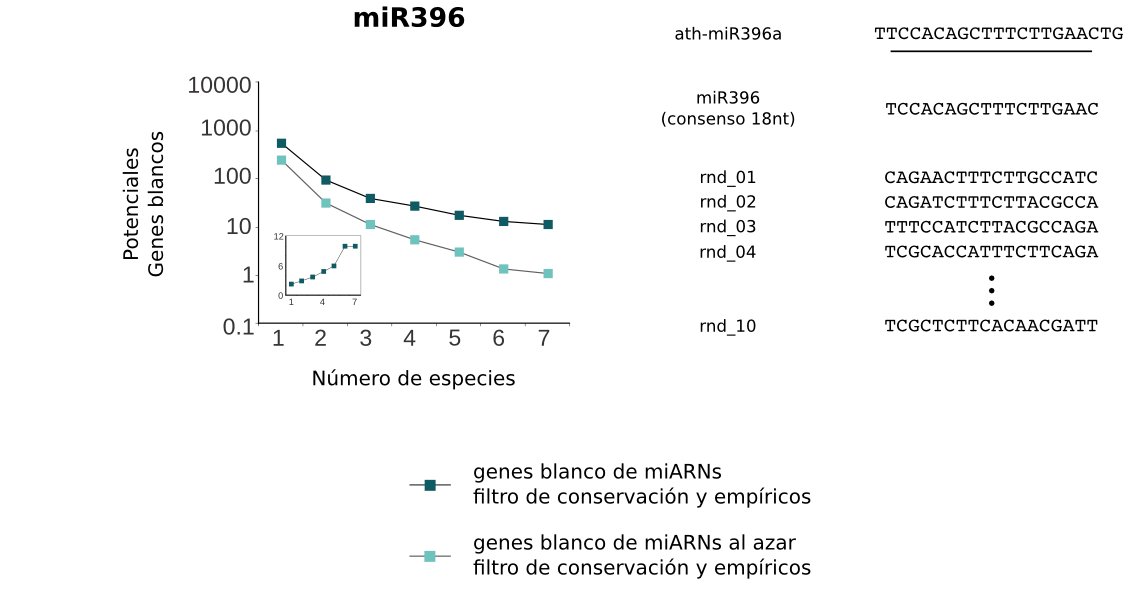
\includegraphics[width=1\textwidth]{img/NAR_fig2_04.png}
	\end{center}
\end{frame}

\begin{frame}{Efecto sinérgico al combinar filtro de conservación evolutiva y empíricos}
%~ pueden estar seleccionando aspectos diferentes de la interacción miARN-gen blanco
	\begin{center}
		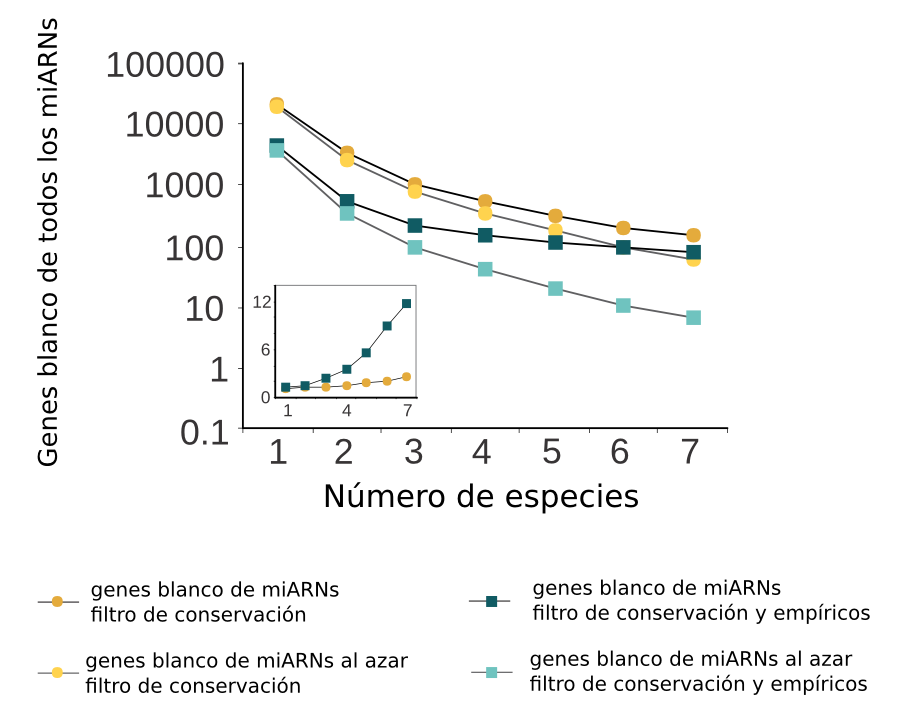
\includegraphics[width=1\textwidth]{img/NAR_fig2_05.png}
	\end{center}
\end{frame}

\begin{frame}{El número de genes blancos candidatos y la relación señal/ruido es variable entre los distintos miARNs}
	\begin{center}
		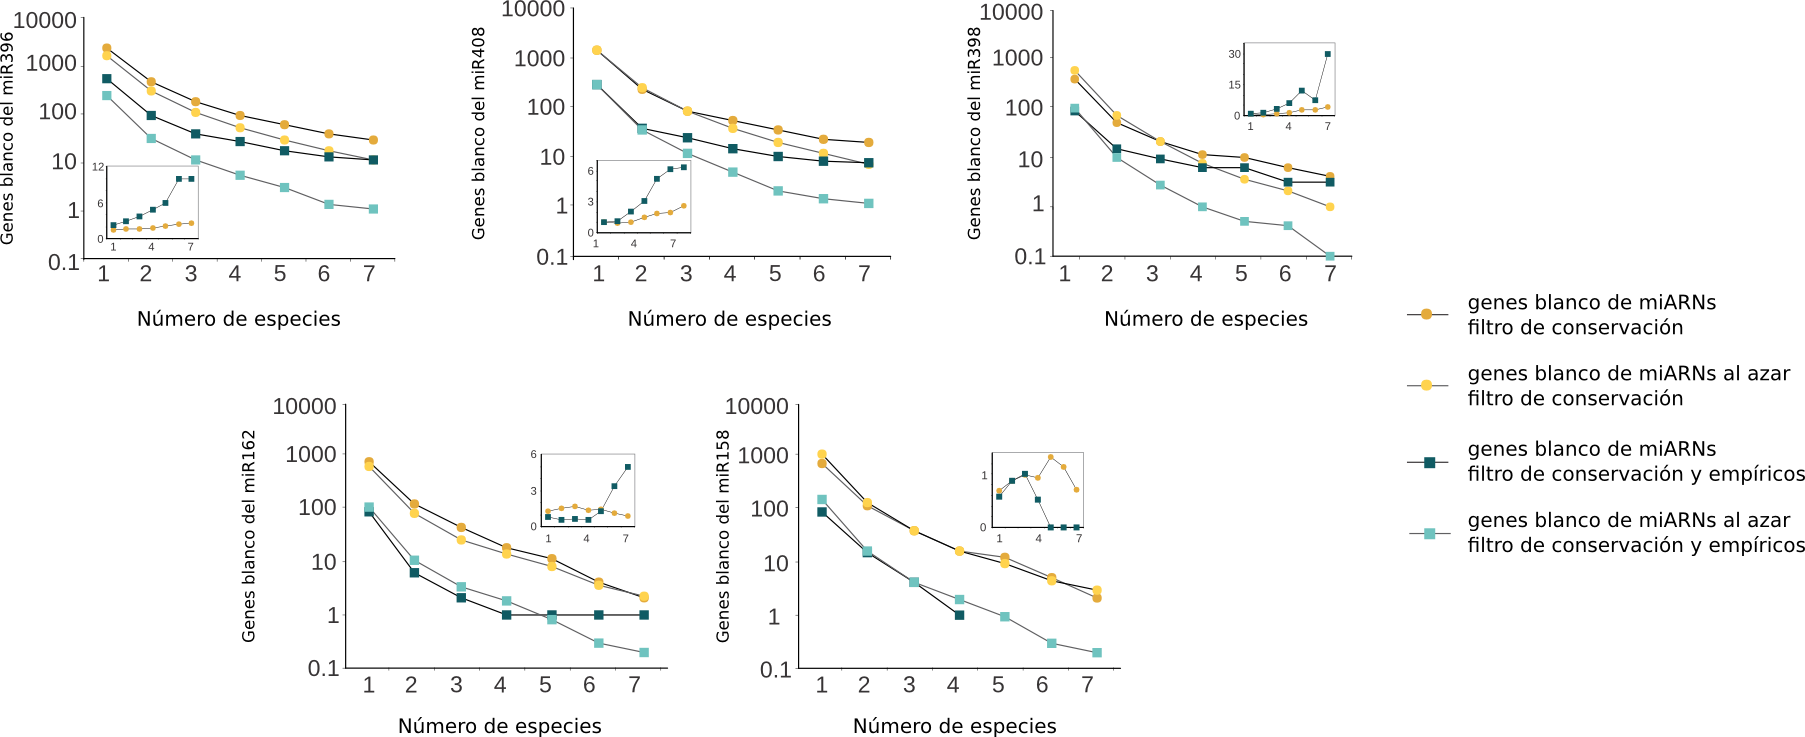
\includegraphics[width=1\textwidth]{img/NAR_fig2_bis.png}
	\end{center}
\end{frame}

\begin{frame}{Potenciales genes blancos utilizando solo conservación evolutiva}
	\begin{center}
		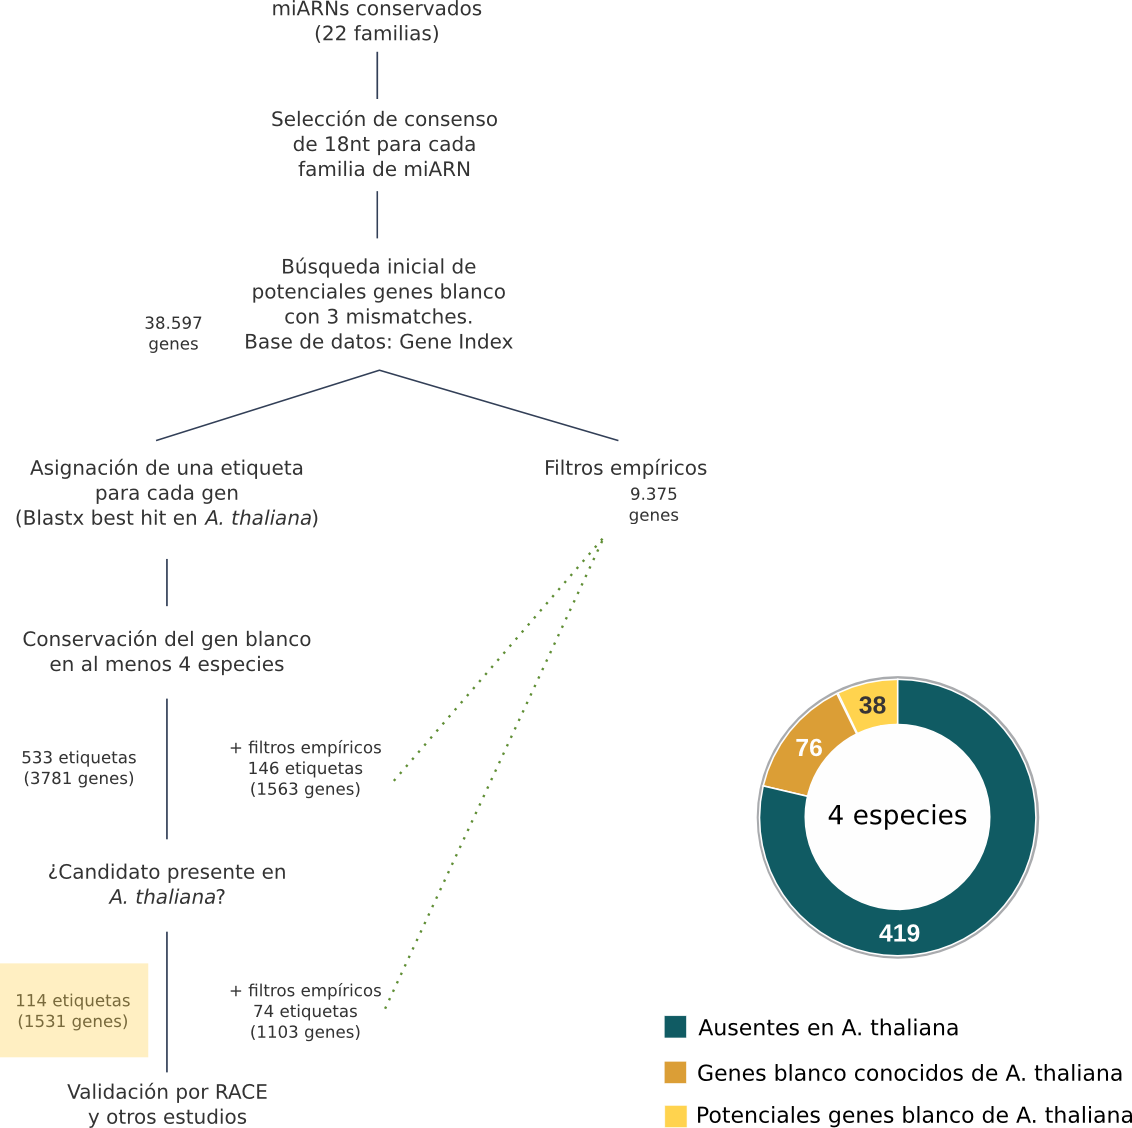
\includegraphics[width=.7\textwidth]{img/NAR_fig01y03.png}
	\end{center}
\end{frame}

\begin{frame}{Se validaron 6 nuevos genes blanco en \textit{A. thaliana}}
	\begin{center}
		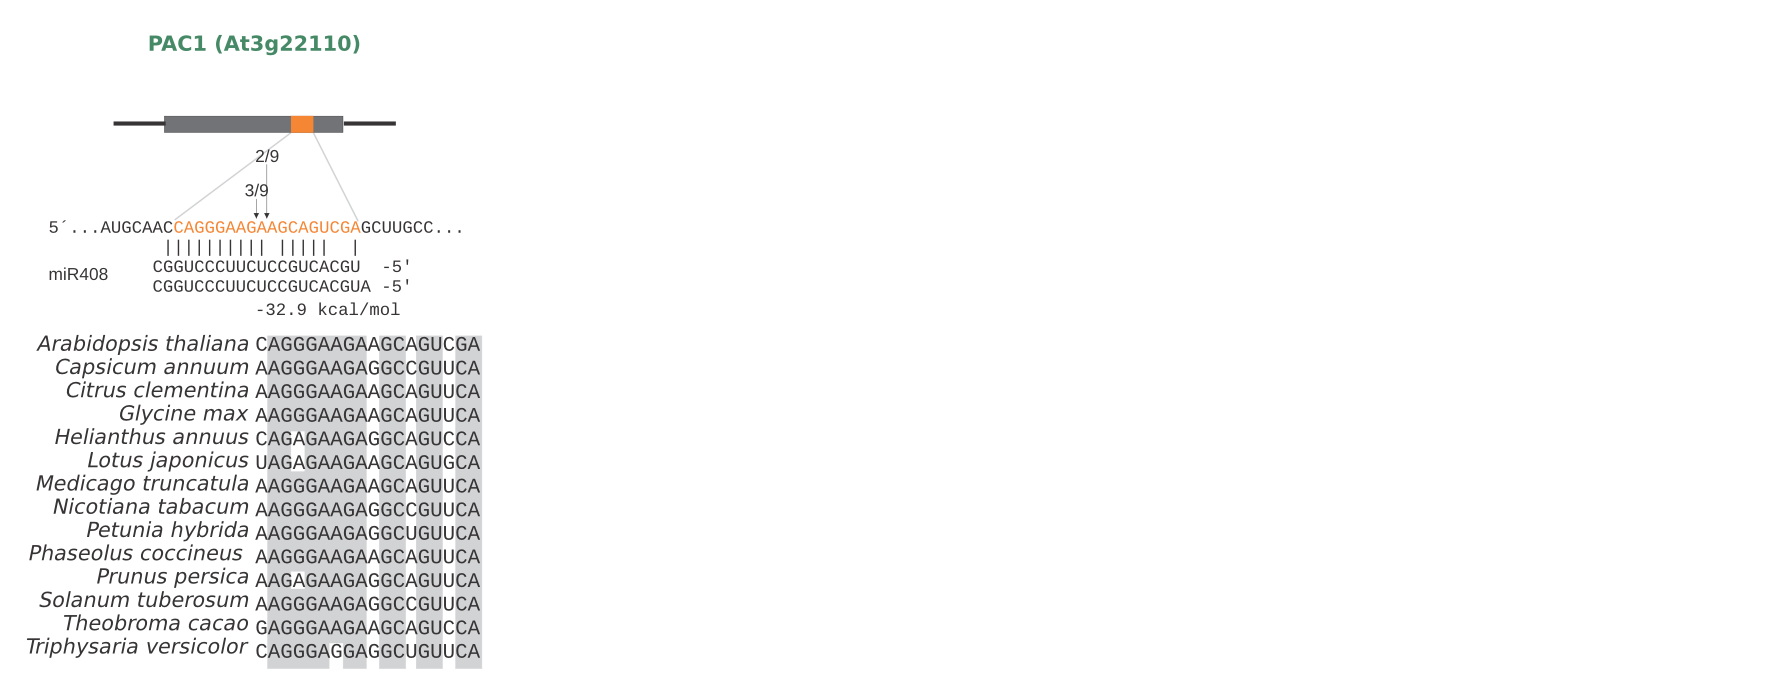
\includegraphics[width=1\textwidth]{img/Figure4_retocada_nueva01.png}
	\end{center}
\end{frame}



\begin{frame}{¿Pueden los miARNs en Angiospermas regular genes específicos de Solanaceae?}
	%~ Superóxido dismutasa
	\begin{center}
		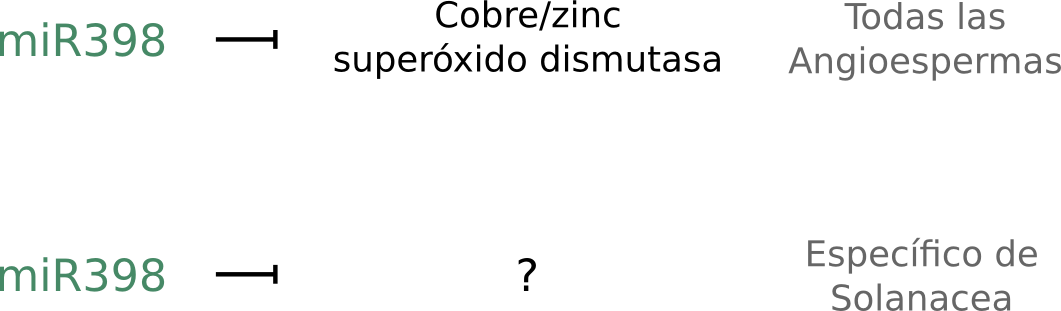
\includegraphics[width=.8\textwidth]{img/miR398_solanaceae.png}
	\end{center}
\end{frame}

\begin{frame}{Identificación de genes blancos específicos de \textit{Solanaceae}}
	\begin{center}
		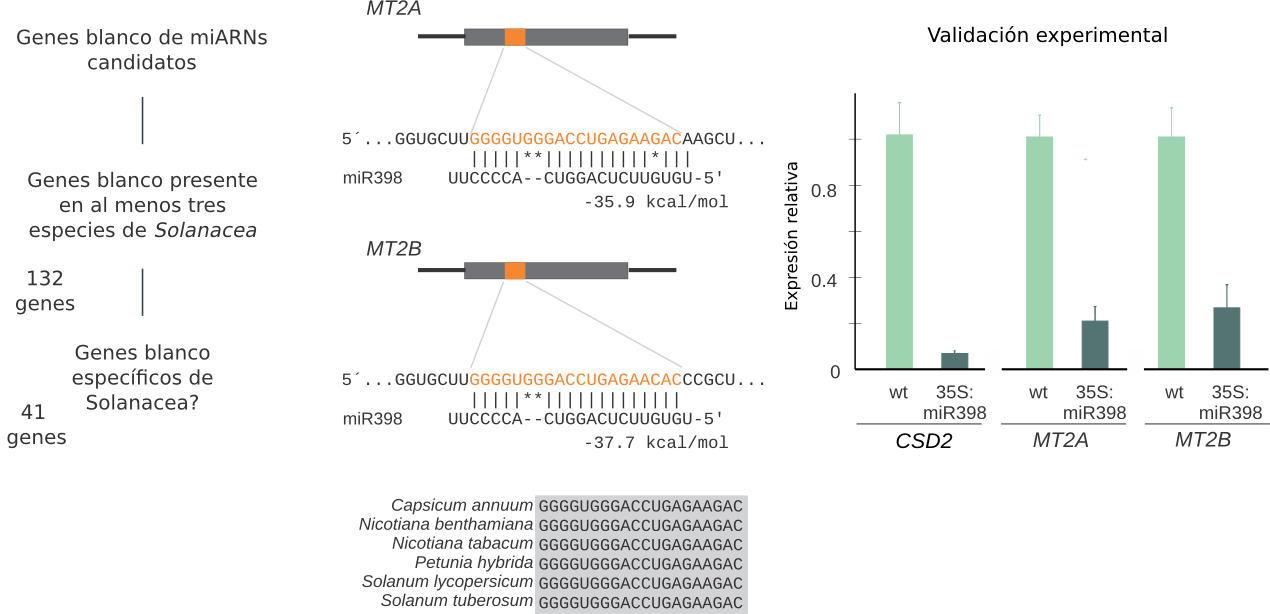
\includegraphics[width=.8\textwidth]{img/Figure6_retocada.png}
	\end{center}
\end{frame}


\begin{frame}{Herramienta web para la predicción de genes blancos regulados por miARNs en plantas}
Desarrollamos ComTAR, que permite realizar la búsqueda de:

\begin{itemize}
    \item<2-> potenciales genes blancos a partir de un miARN.
    \item<2-> familias de potenciales genes blancos de un miARN.
    \item<2-> un gen de interés para ver si es potencial gen blanco de algún miARN conservado
    \item<2-> nuevos ARNs pequeños
\end{itemize}
    \begin{center}
        \uncover<3->{\href{http://rnabiology.ibr-conicet.gov.ar/comtar}{\beamergotobutton{http://rnabiology.ibr-conicet.gov.ar/comtar}}}
    \end{center}
\end{frame}

\begin{frame}{Potenciales genes blancos del miR398}
	\begin{center}
		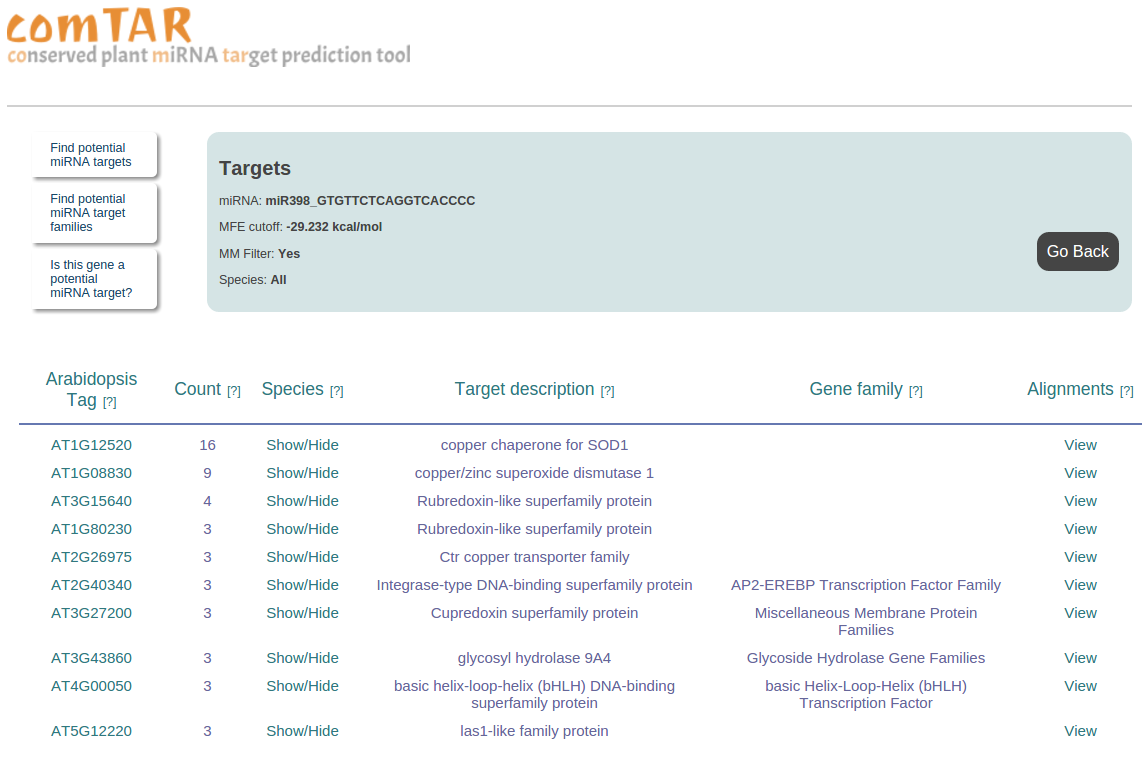
\includegraphics[width=.8\textwidth]{img/comTAR_find_targets.png}
	\end{center}
\end{frame}

\begin{frame}{ComTAR permite visualizar el alineamiento, energía de hibridación en cada especie}
	\begin{center}
		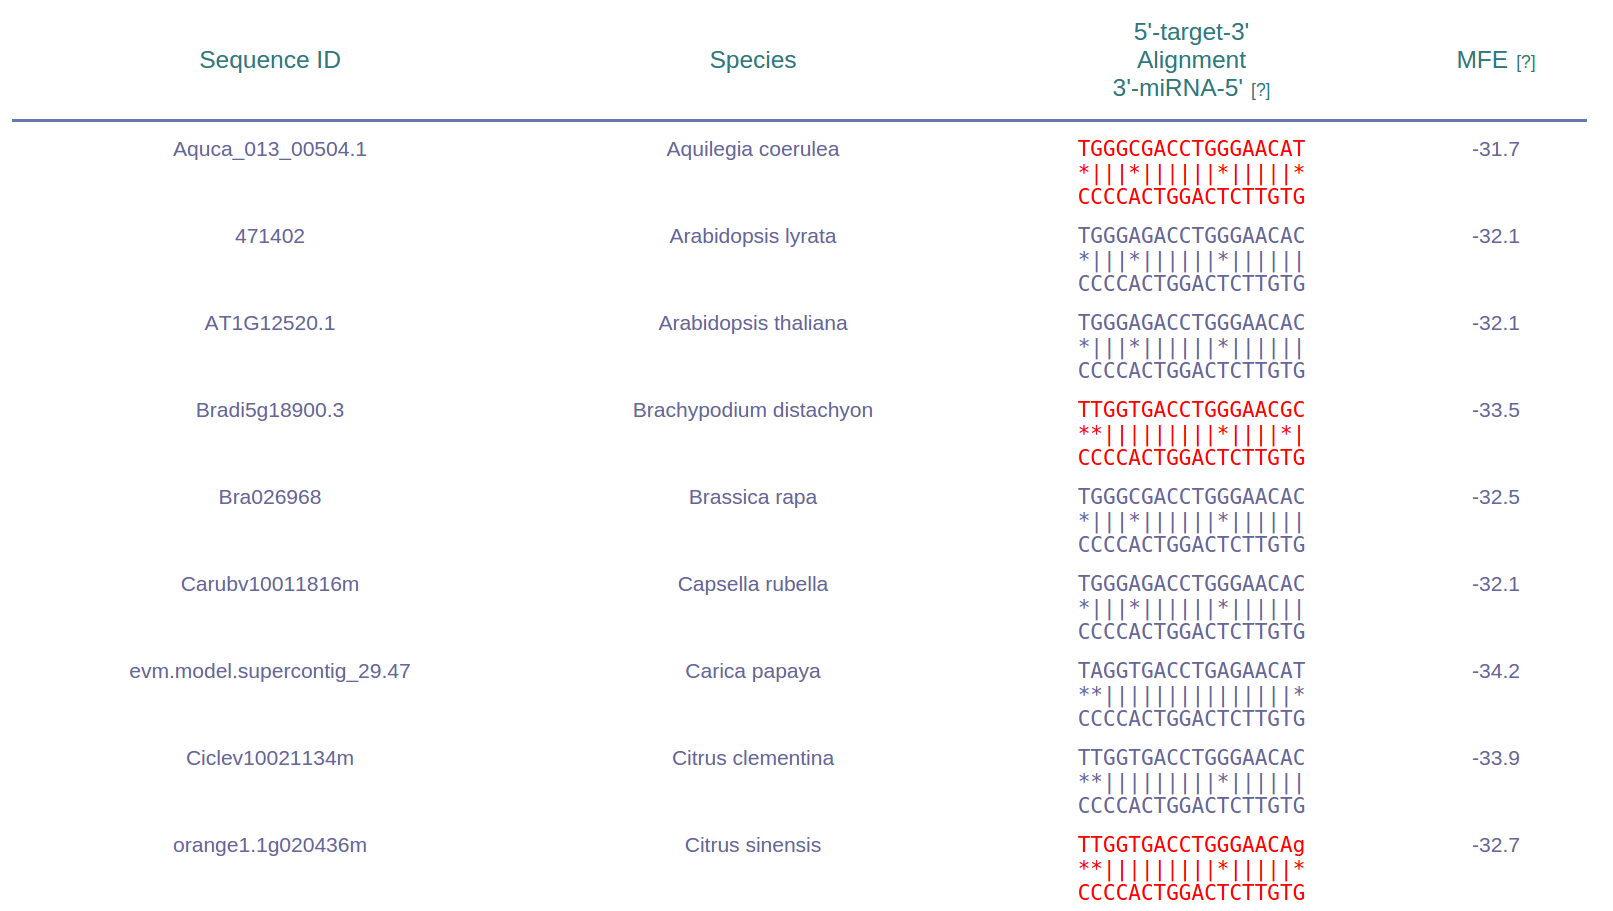
\includegraphics[width=.7\textwidth]{img/comTAR_fig2.png}
	\end{center}
\end{frame}

\begin{frame}{Conclusiones I}
	\begin{itemize}
        \item<1-> Diseñamos una estrategia para identificar genes blancos regulados por miARNs en plantas, basado en la conservación evolutiva del par miARN-gen blanco.
        \item<2-> Identificamos nuevos genes blancos en \textit{A. thaliana} y se validaron experimentalmente varios de ellos.
        %~ a pesar de que este sistema ya había sido estudiado en detalles en distintos enfoques genómicos. 
        \uncover<2->{   \begin{center}
                            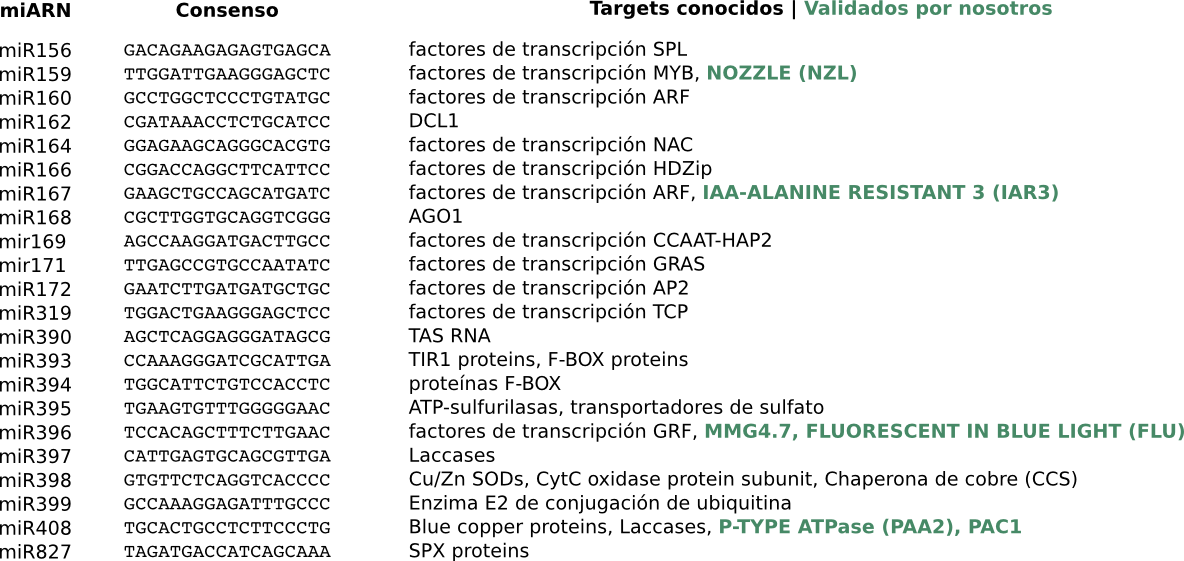
\includegraphics[width=.69\textwidth]{img/tabla_targets.png}
                        \end{center}
        }
	\end{itemize}
\end{frame}


\begin{frame}{Conclusiones I}
	\begin{itemize}
        \item<1-> Diseñamos una estrategia para identificar genes blancos regulados por miARNs en plantas, basado en la conservación evolutiva del par miARN-gen blanco.
        \item<1-> Identificamos nuevos genes blancos en \textit{A. thaliana} y se validaron experimentalmente varios de ellos.
        \item<1-> Esta estrategia puede ser utilizada para identificar genes blancos presentes en un grupo específico de especies.
        \item<2-> Interacciones miARN-gen blanco conservadas probablemente participen en procesos biológicos relevantes.
        \item<3-> Desarrollamos una herramienta web denominada comTAR para predecir potenciales genes blancos regulados por miARNs en plantas.
	\end{itemize}
\end{frame}

\subsection{Resultados 2}

\begin{frame}{Objetivos específicos}
    \setbeamercovered{transparent=25}
		\pause
		\begin{itemize}
            \item<-1> Diseñar una estrategia para la identificación de genes blancos regulados por miARNs.
			\item<-2> Caracterizar precursores de miARNs en distintas especies que tengan mecanismos de procesamiento distintos.
			\item<-1> Caracterizar la relación entre la evolución de los precursores de miARNs en plantas y los mecanismos de procesamiento determinados previamente.
        \end{itemize}
\end{frame}

%~ Estudios genómicos sobre la biogénesis de precursores de miARNs en plantas.

\begin{frame}{Precursores en plantas son muy variables en tamaño y forma}
	\begin{center}
		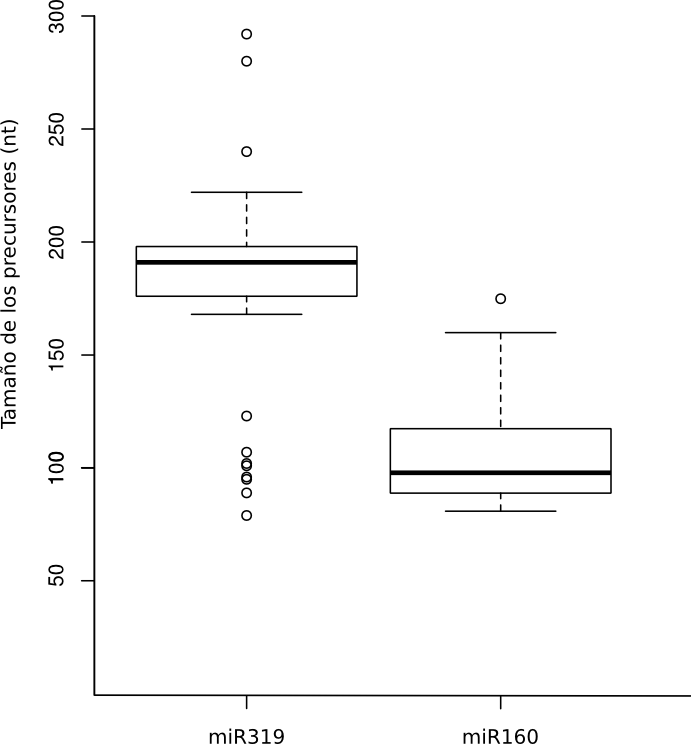
\includegraphics[width=.5\textwidth]{img/hairpin_distribution.png}
	\end{center}
\end{frame}

\begin{frame}{Bibliotecas SPARE para estudios genómicos de biogénesis de miARNs en plantas}
\begin{columns}
    \begin{column}{0.3\textwidth}
		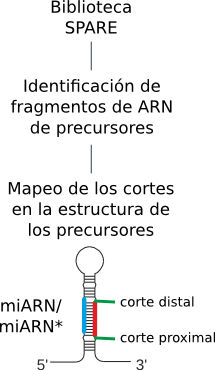
\includegraphics[width=.6\textwidth]{img/GR_fig1C.png}
    \end{column}
    \begin{column}{0.7\textwidth}
        \uncover<2->{
            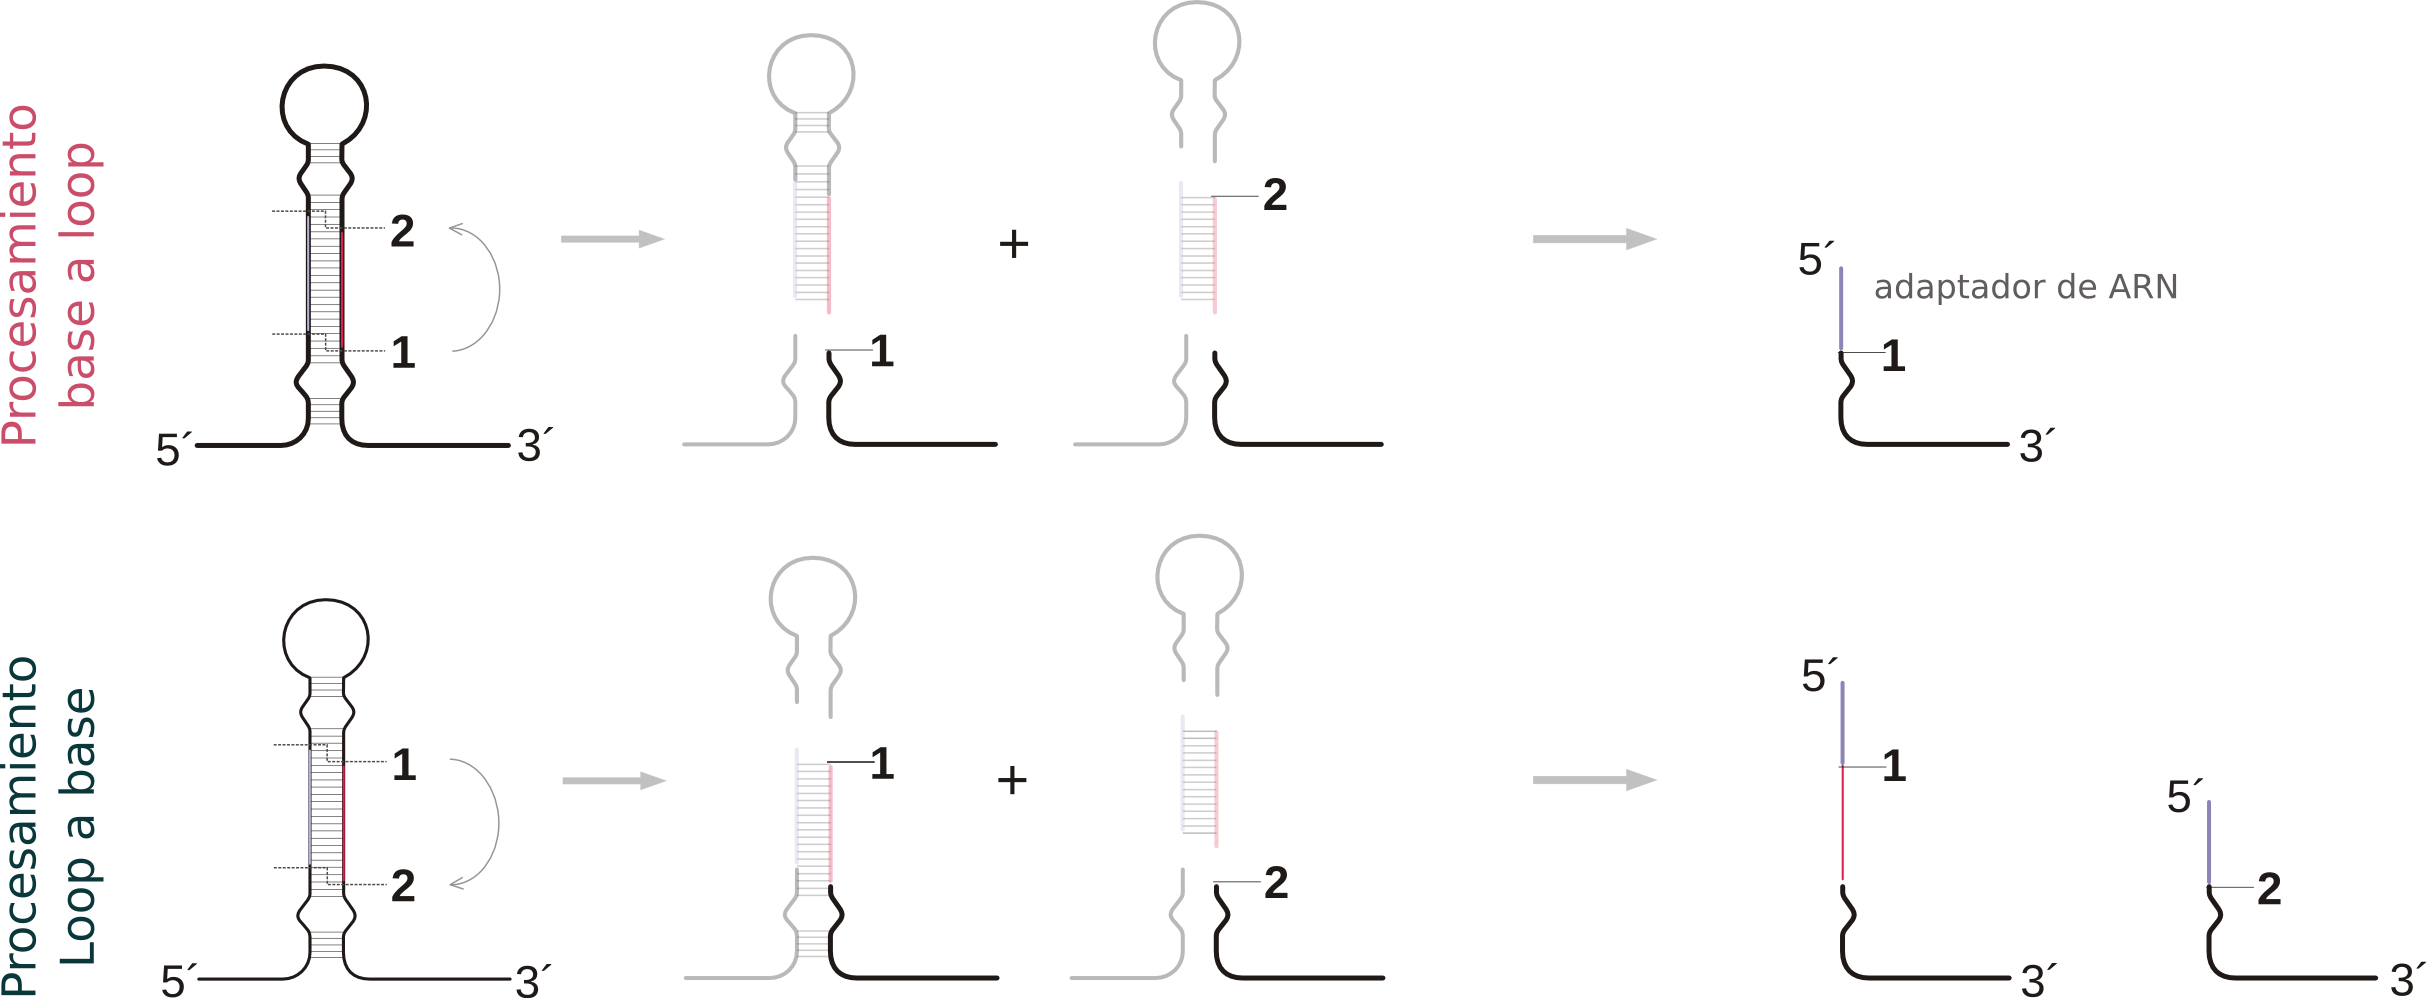
\includegraphics[width=1\textwidth]{img/SPARE_tecnica.png}
        }
    \end{column}
\end{columns}
\end{frame}


\begin{frame}{Los precursores que se procesan desde la base tienen un sólo pico de señal en las bibliotecas de SPARE}
	\begin{center}
		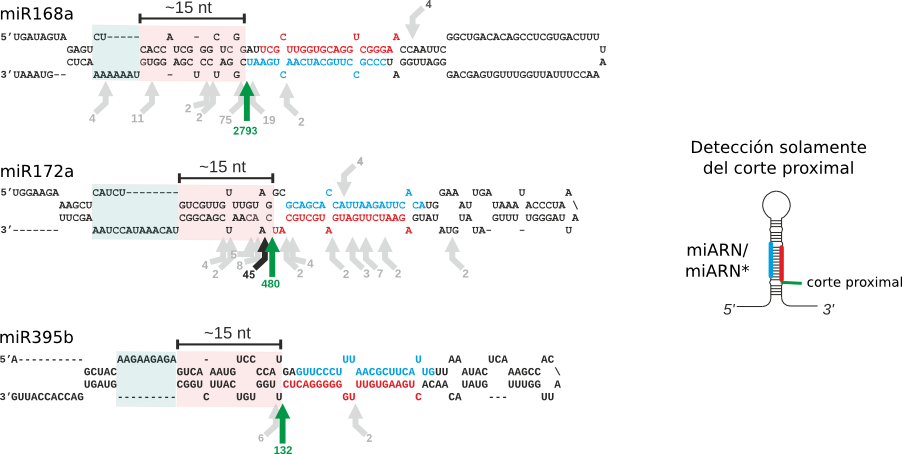
\includegraphics[width=.8\textwidth]{img/GR_fig2A.png}
	\end{center}
\end{frame}

\begin{frame}{Los precursores que se procesan desde la base tienen al menos dos picos de señal en las bibliotecas de SPARE}
	\begin{center}
		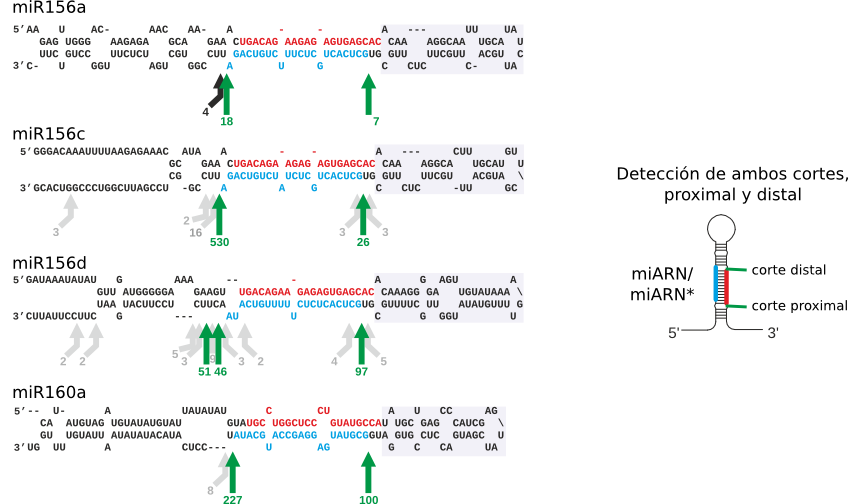
\includegraphics[width=.7\textwidth]{img/GR_fig4A.png}
	\end{center}
\end{frame}


\begin{frame}{Bibliotecas de SPARE}
\begin{table}[]
    \centering
    \tiny
    \begin{tabular}{llccc}
        \multicolumn{1}{c}{\textbf{Bibliotecas}} & \multicolumn{1}{c}{\textbf{Muestras}} &  \textbf{\begin{tabular}[c]{@{}c@{}}Secuencias\\ totales \\\end{tabular}} &  \textbf{\begin{tabular}[c]{@{}c@{}}Secuencias\\ que mapean\\ los precursores\end{tabular}} &  \textbf{\begin{tabular}[c]{@{}c@{}}Secuencias únicas\\ que mapean\\ los precursores\end{tabular}} \\
        col\_2AB                                 & Col-0 réplica 1. Control de fiery y hyl1 & 13911694                                                                 & 80166                                                                                      & 308                                                                                               \\
        col\_3AB                                 & Col-0 réplica 2. Control de fiery y hyl1 & 16618008                                                                 & 126556                                                                                     & 426                                                                                               \\
        Col\_AD                                  & Col-0 réplica 1. Control de se           & 13758567                                                                 & 119368                                                                                     & 496                                                                                               \\
        Col\_BC                                  & Col-0 réplica 2. Control de se           & 14648459                                                                 & 241973                                                                                     & 553                                                                                               \\
        FIERY\_1AB                               & fiery réplica 1                          & 9832923                                                                  & 470789                                                                                     & 1655                                                                                              \\
        FIERY\_4                                 & fiery réplica 2                          & 23529725                                                                 & 821562                                                                                     & 1752                                                                                              \\
        HYL\_1                                   & hyl1 réplica 1                           & 10171629                                                                 & 45653                                                                                      & 316                                                                                               \\
        HYL\_2                                   & hyl1 réplica 2                           & 8864406                                                                  & 35860                                                                                      & 320                                                                                               \\
        SE\_BD                                   & se réplica 1                             & 15291993                                                                 & 299513                                                                                     & 639                                                                                               \\
        SE\_CE                                   & se réplica 1                             & 25296809                                                                 & 510438                                                                                     & 693                                                                                              
    \end{tabular}
\end{table}
\end{frame}


\begin{frame}{Visualización de precursores procesados desde la base}
	\begin{center}
		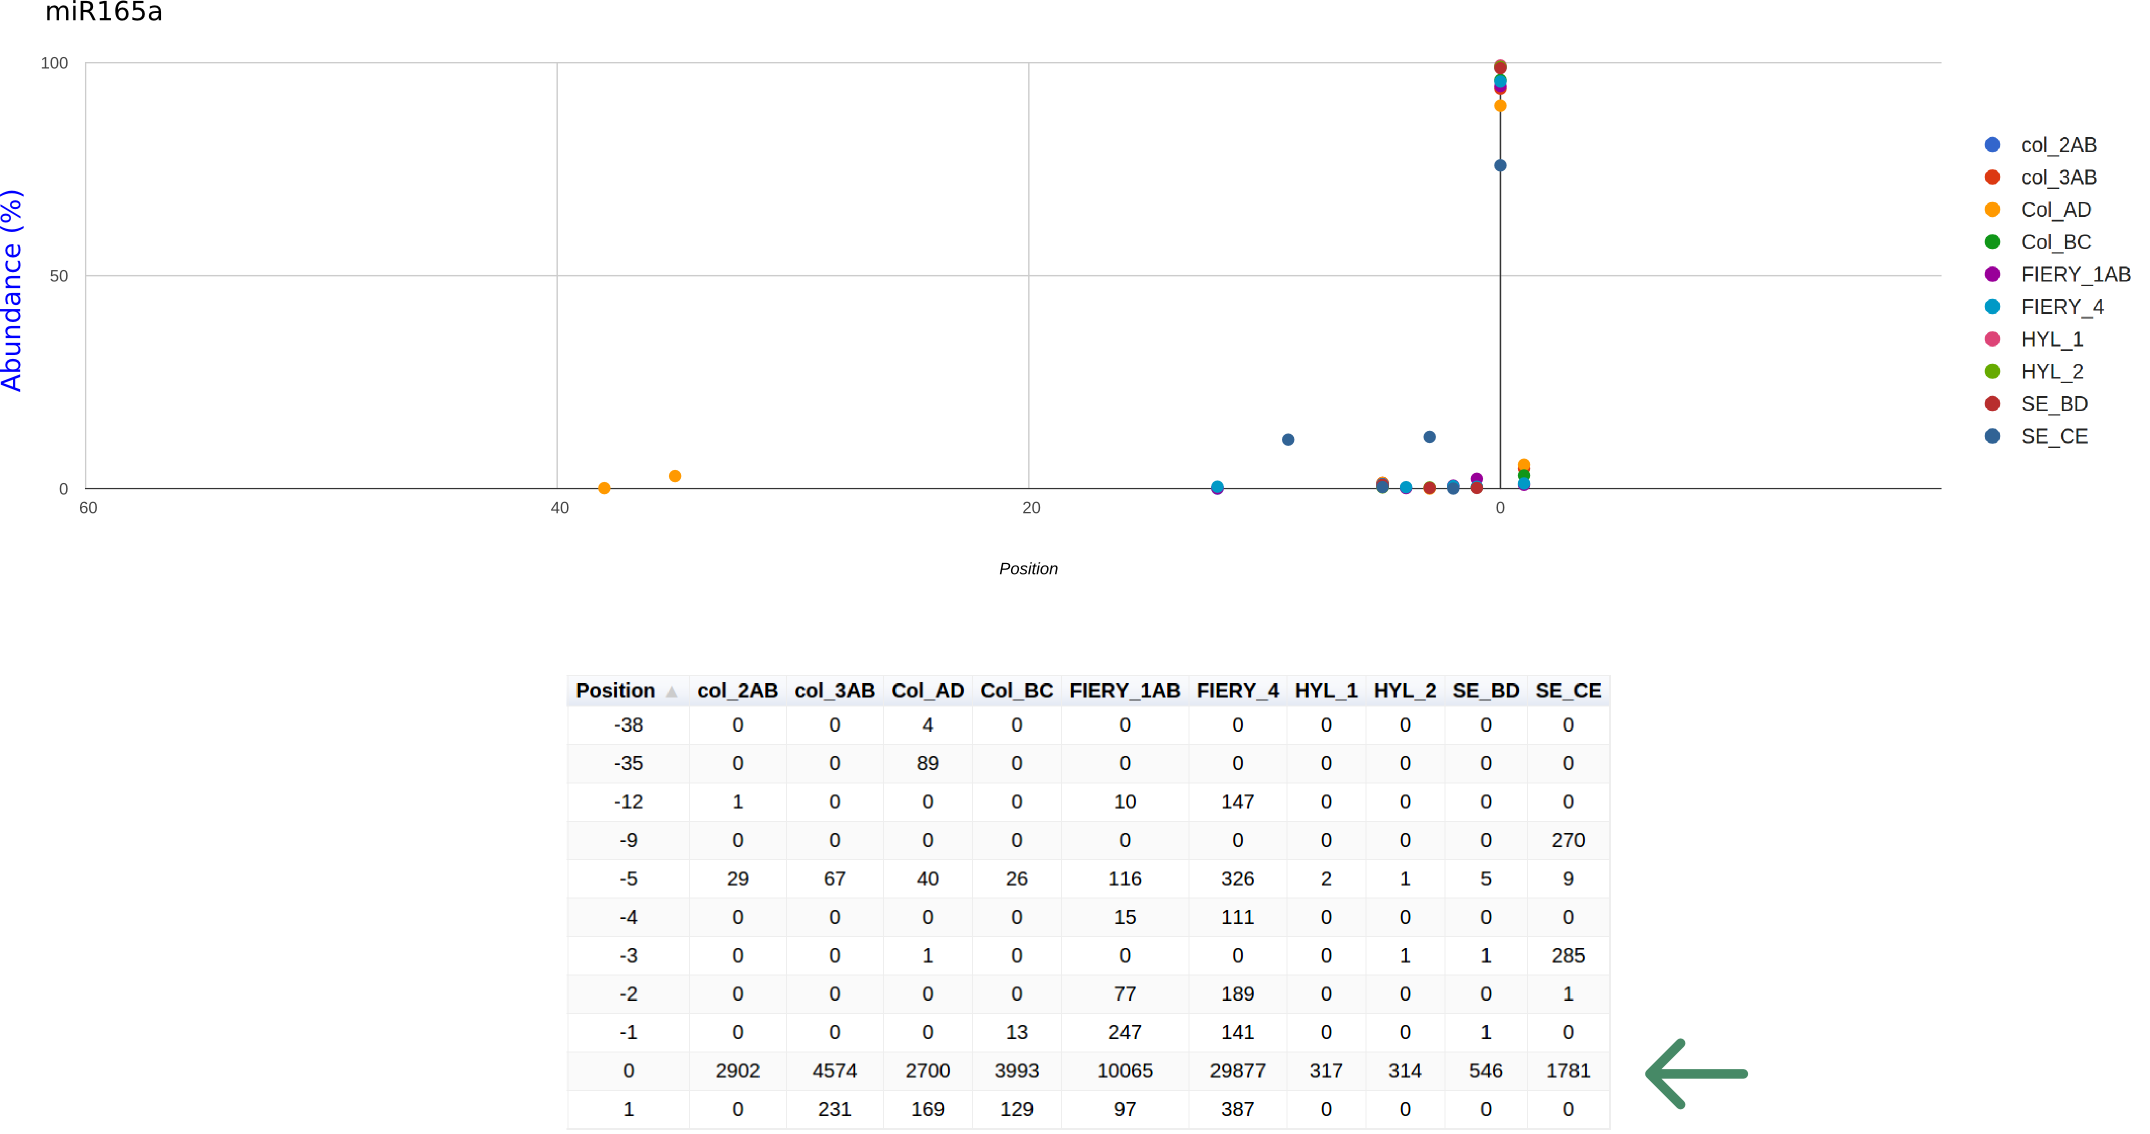
\includegraphics[width=1\textwidth]{img/miR165a_SPARE.png}
	\end{center}
\end{frame}

\begin{frame}{Visualización de precursores procesados desde el loop}
	\begin{center}
		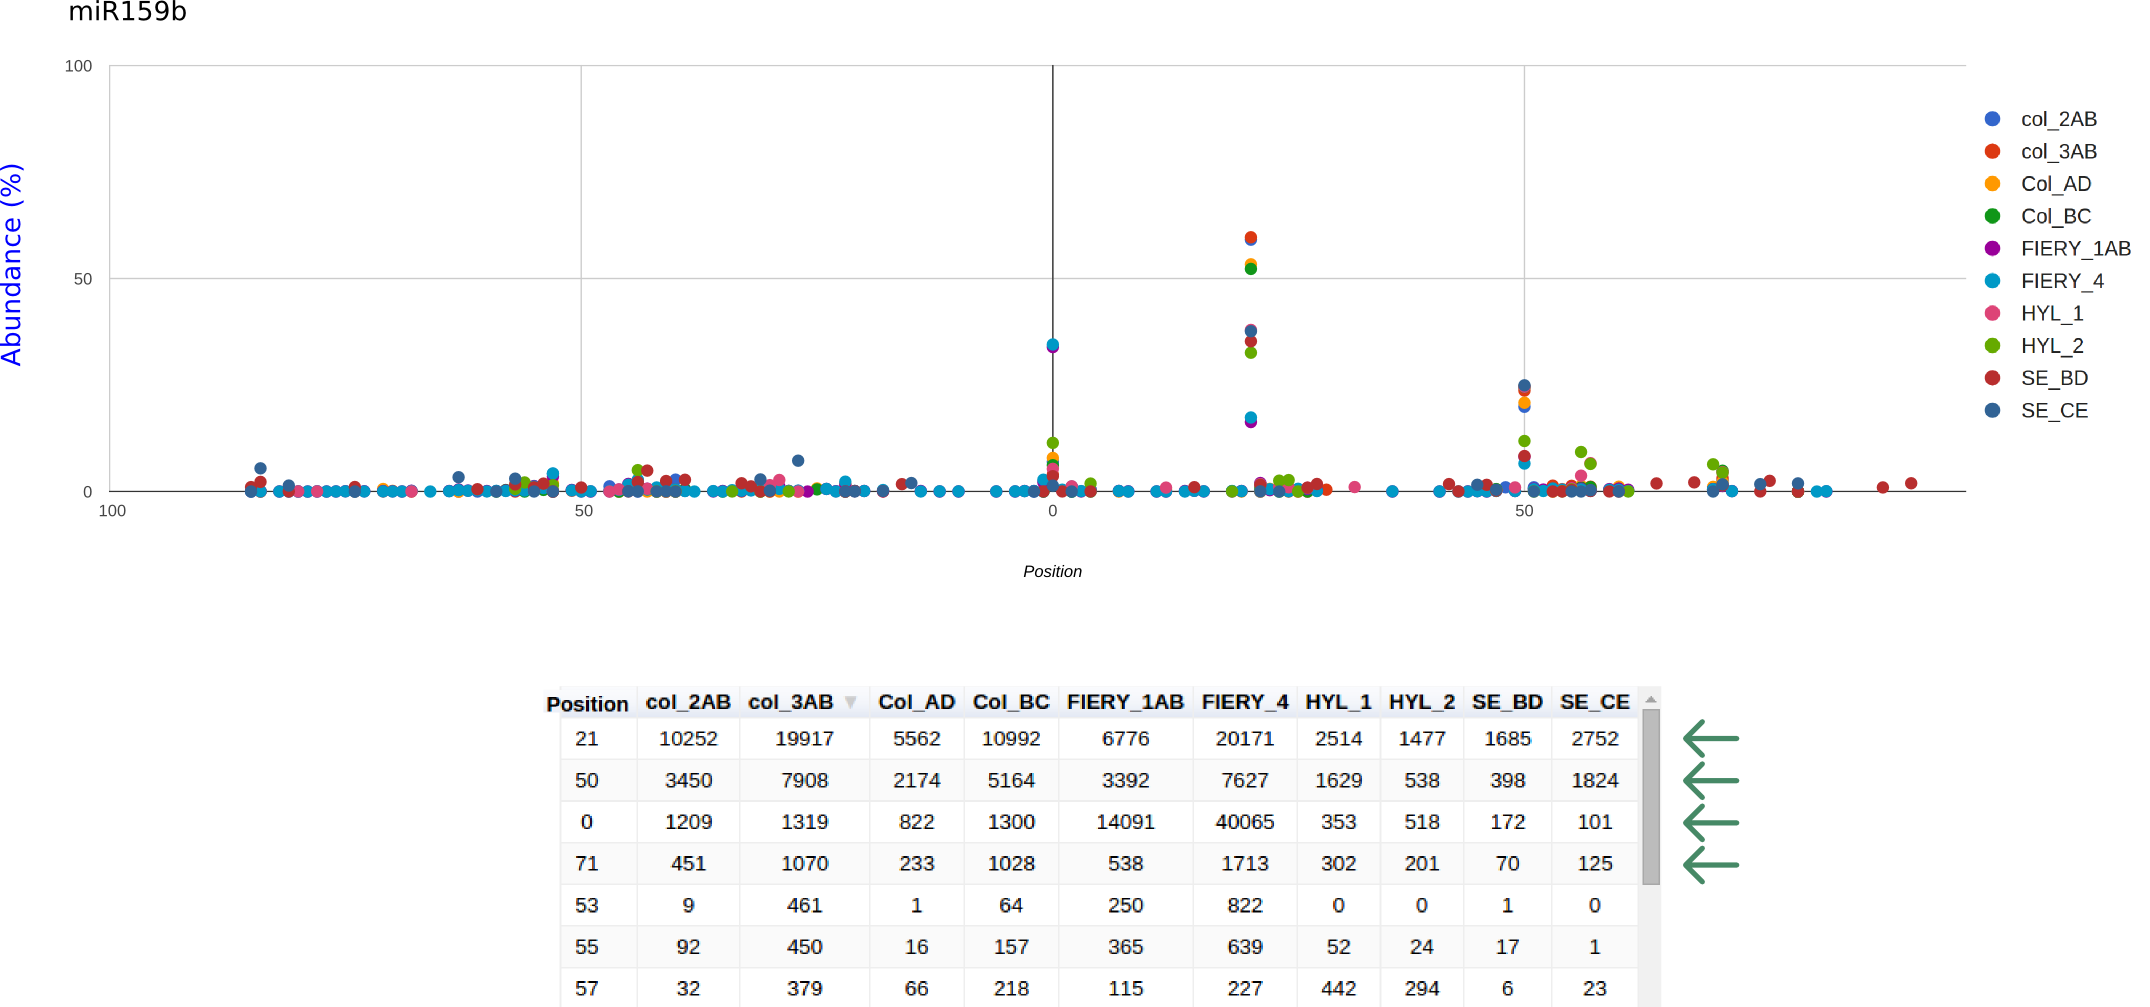
\includegraphics[width=1\textwidth]{img/miR159b_SPARE.png}
	\end{center}
\end{frame}


\begin{frame}{Conclusiones II}
	\begin{center}
		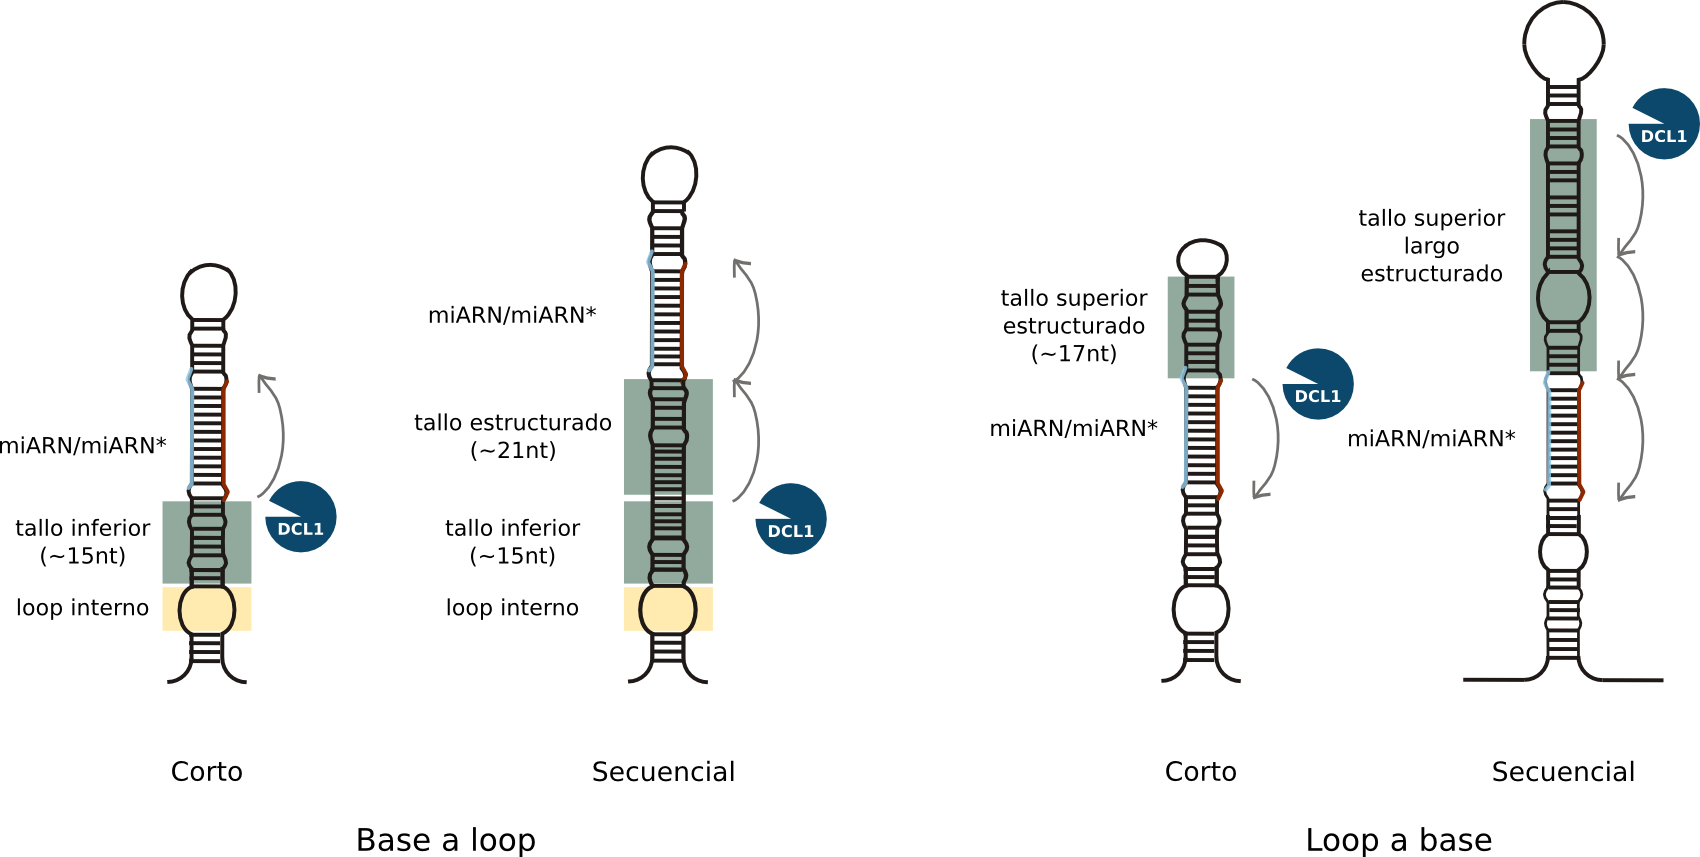
\includegraphics[width=1\textwidth]{img/mecanismos.png}
	\end{center}
\end{frame}


%~ \begin{frame}{Conclusiones II}
%~ \begin{itemize}
    %~ \item En los precursores con un mecanismo \textbf{corto de base a loop}, un loop interno seguido por un tallo inferior de $\sim$15nt especifica la posición del primer corte.
        %~ Esta estructura se encuentra en la mayoría de familias de miARNs.
        %~ A pesar de que el tallo puede contener bulges, la transición de un loop interno (simple hebra) al tallo inferior es bastante marcada, y tres pares de bases apareadas generalmente definen el comienzo del tallo inferior del precursor.
        %~ El segundo corte procede a una distancia fija de $\sim$21 nt desde la posición del primer corte.
    %~ \item En los precursores con un mecanismo \textbf{secuencial de base a loop} (ej: familia del miR169), el primer corte procede como en los cortos de base a loop, pero luego son necesario dos cortes más para liberar el miARN, generando en el proceso niveles bajos de RNA pequeños adicionales.
    %~ \item En los precursores con un mecanismo \textbf{cortos de loop a base} (ej: familia del miR156 y miR160), el procesamiento es guiado por un tallo superior, y son necesarios dos cortes para liberar el miARN maduro.
        %~ La región terminal de estos precursores tienen una largo conservado de $\sim$42 donde incluye un loop pequeñ.
    %~ \item En los precursores con un mecanismo \textbf{secuencial de loop a base} (ej: familia del miR319 y miR159), cuatro cortes secuenciales por DCL1 son los encargados de procesar los precursores de miARNs.
        %~ En general muestran un tallo largo superior, del cual otros ARNs pequeños son generados.
%~ \end{itemize}
%~ \end{frame}

\subsection{Resultados 3}

\begin{frame}{Objetivos específicos}
    \setbeamercovered{transparent=25}
		\pause
		\begin{itemize}
            \item<-1> Diseñar una estrategia para la identificación de genes blancos regulados por miARNs.
			\item<-1> Caracterizar precursores de miARNs en distintas especies que tengan mecanismos de procesamiento distintos.
			\item<-2> Caracterizar la relación entre la evolución de los precursores de miARNs en plantas y los mecanismos de procesamiento determinados previamente.
        \end{itemize}
\end{frame}


\begin{frame}{Especies utilizadas de Phytozome (30 dicotiledóneas y 6 monocotiledóneas)}
	\begin{center}
		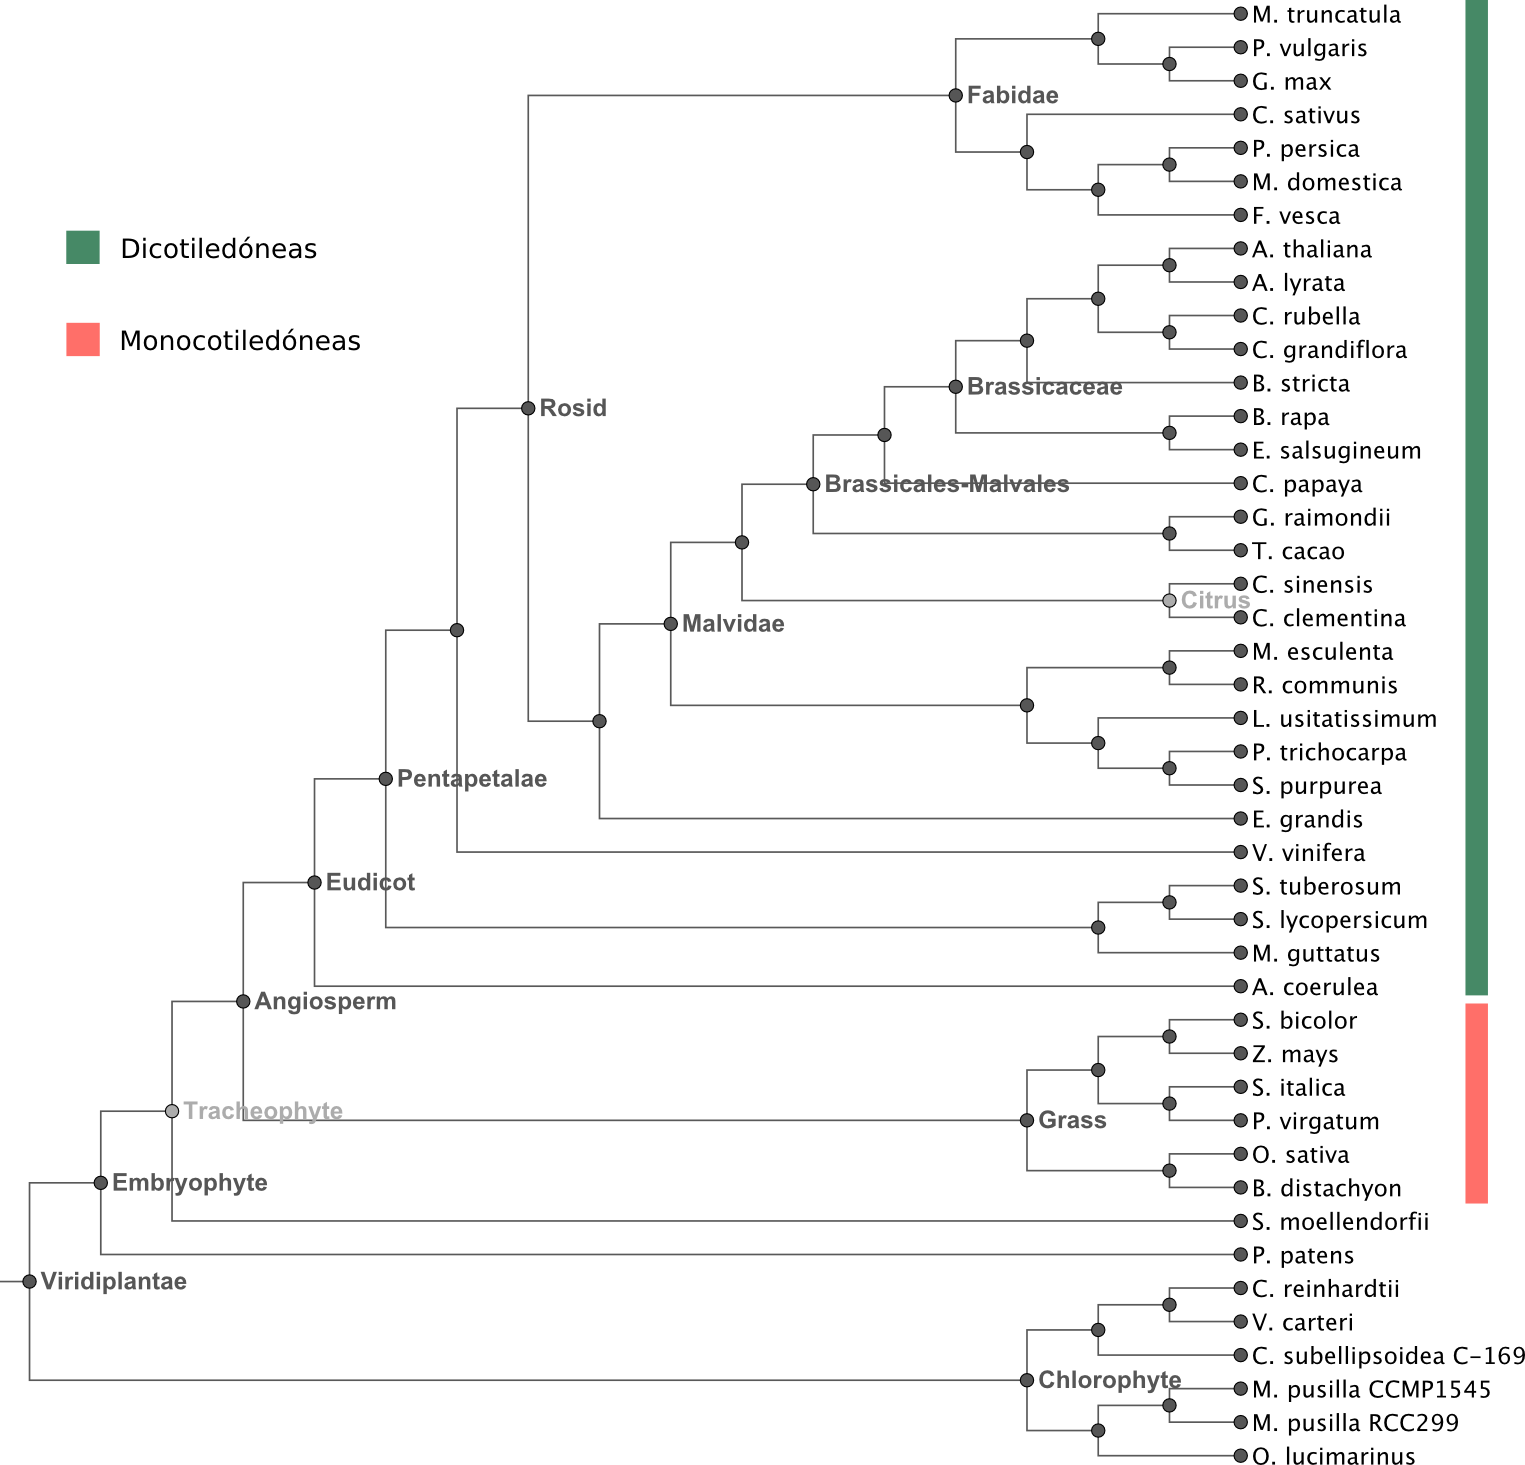
\includegraphics[width=.6\textwidth]{img/treePhytozome.png}
	\end{center}
\end{frame}


\begin{frame}{Dificultades para estudiar precursores de miARNs en distintas especies}
    Anotación arbitraria en miRBASE (Base de datos de secuencias y anotación de miARNs).
    \begin{itemize}
        \item Longitud de precursores.
        \item Definición de ortólogos
    \end{itemize}
\end{frame}

\begin{frame}{¿Cuál es el ortólogo en otras especies?}
	\begin{center}
		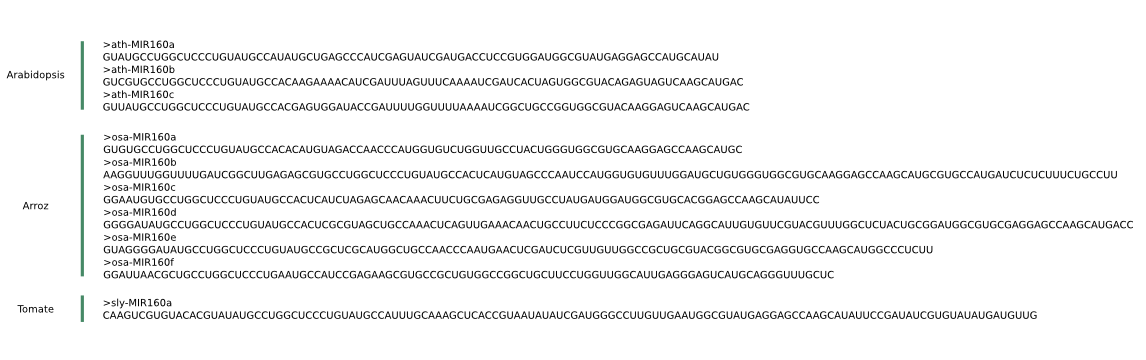
\includegraphics[width=1\textwidth]{img/ortologos01.png}
	\end{center}
\end{frame}

    %~ Comenzamos nuestro análisis con una definición arbitraria de los precursores de plantas incluyendo 150 nt fuera del par miARN/miARN*.
    %~ Para cada miembro de cada familia de A. thaliana no es trivial asignarle un ortólogo en otra especie teniendo en cuenta la anotación de miRBase. 
    
    
    %~ IMPORTANTE
    %~ Por esto, realizamos una búsqueda de ortólogos para cada miembro de cada familia de \textit{A. thaliana} utilizando como criterio la técnica de Blast recíproco.


\begin{frame}{Conservación de la secuencia primaria del miR172a en distintas especies}
	\begin{center}
		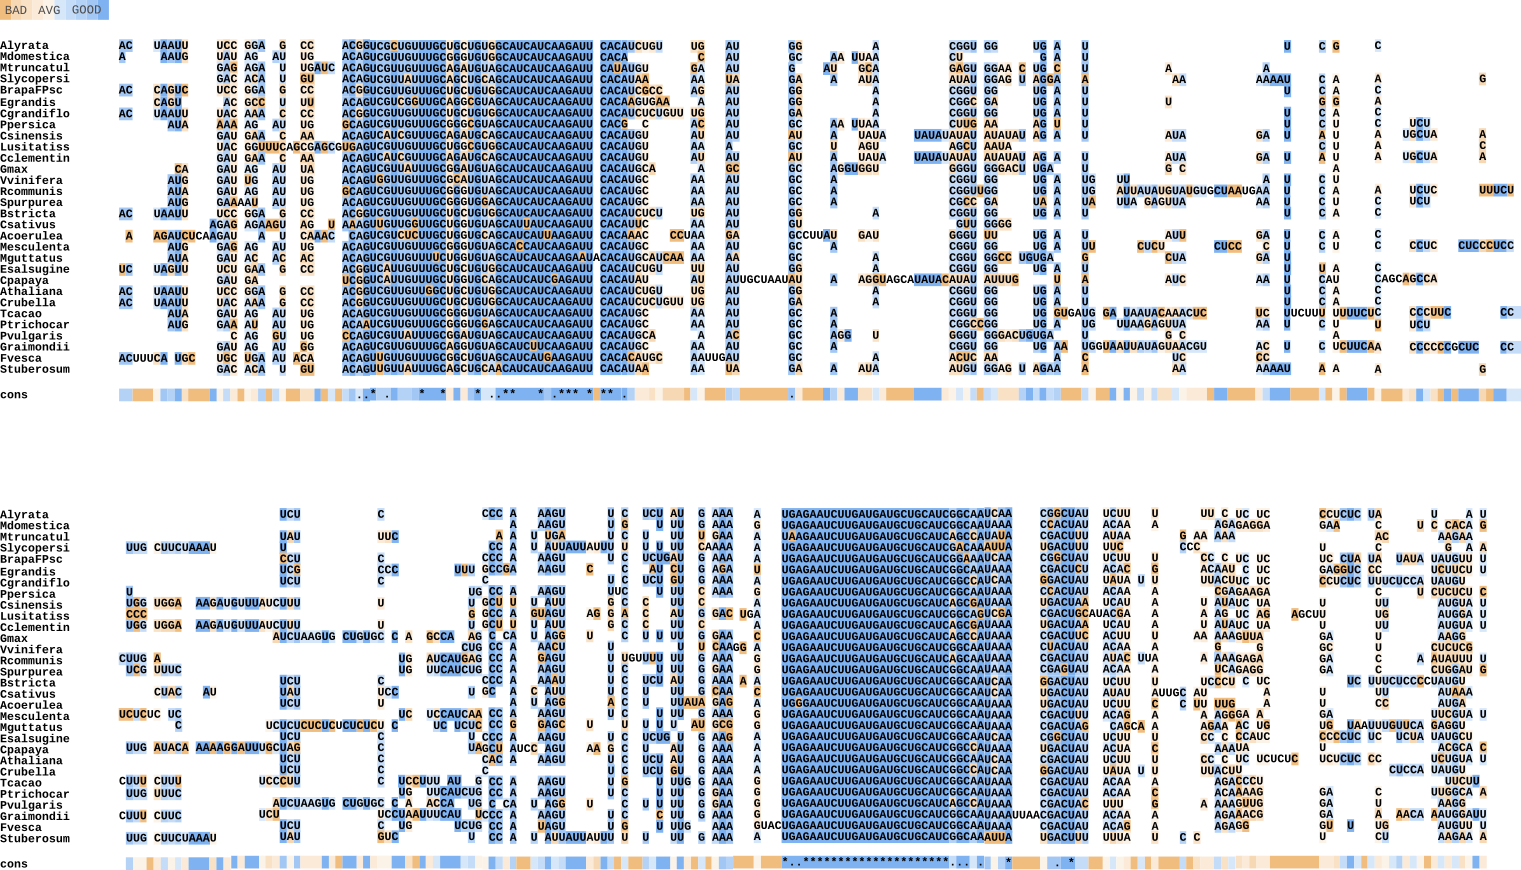
\includegraphics[width=1\textwidth]{img/miR172a_tcoffee_01.png}
	\end{center}
\end{frame}

\begin{frame}{El miR172a maduro y el miR172a* están conservados en las distintas especies}
	\begin{center}
		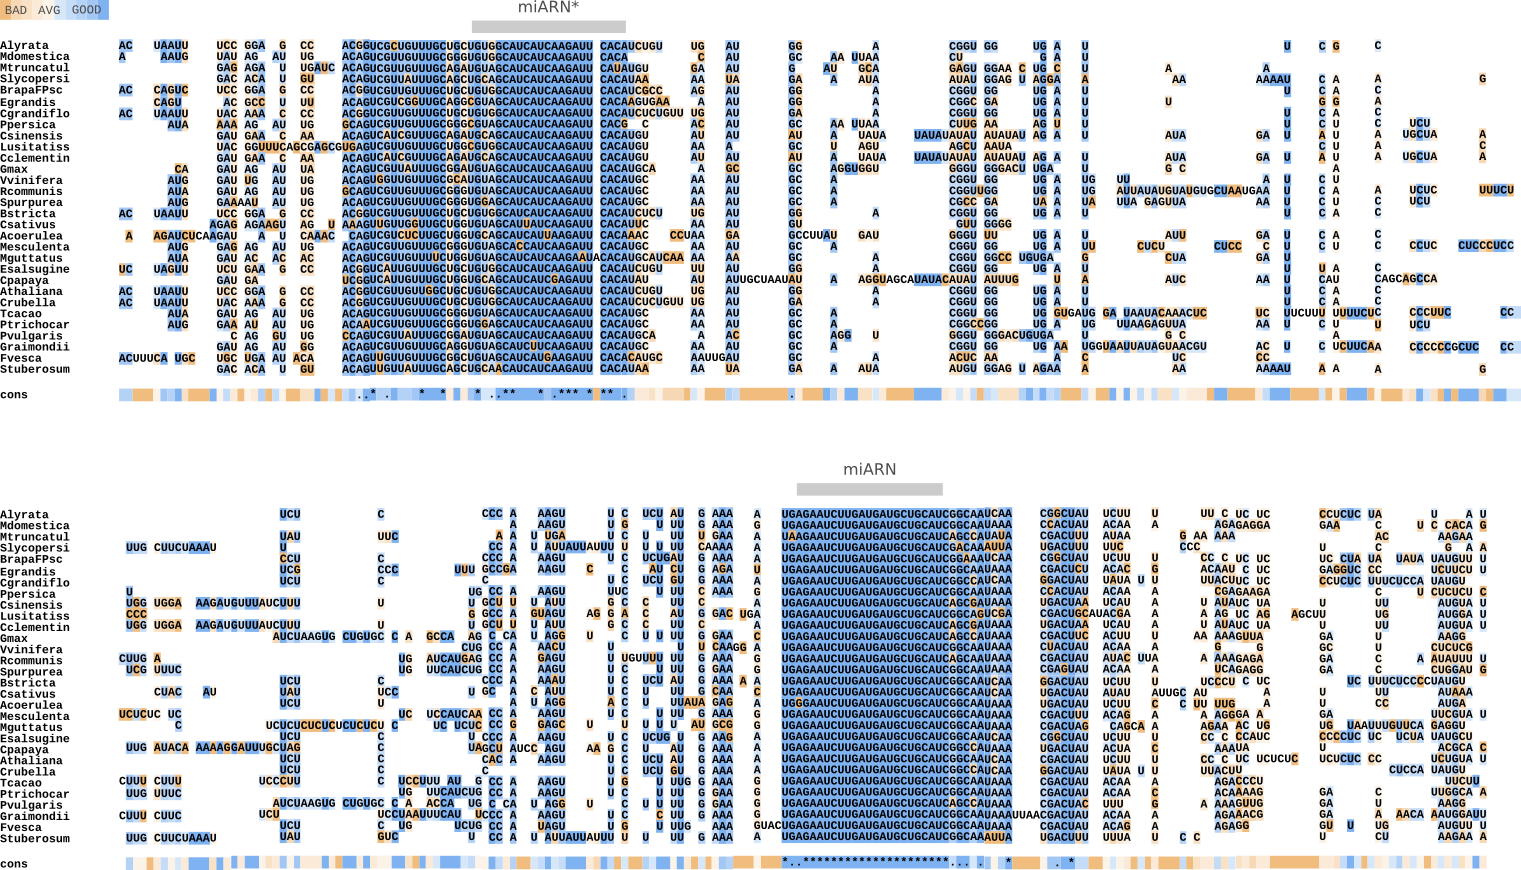
\includegraphics[width=1\textwidth]{img/miR172a_tcoffee_02.png}
	\end{center}
\end{frame}

\begin{frame}{Cola de conservación hacia la izquierda del miARN y hacia la derecha del miARN*}
	\begin{center}
		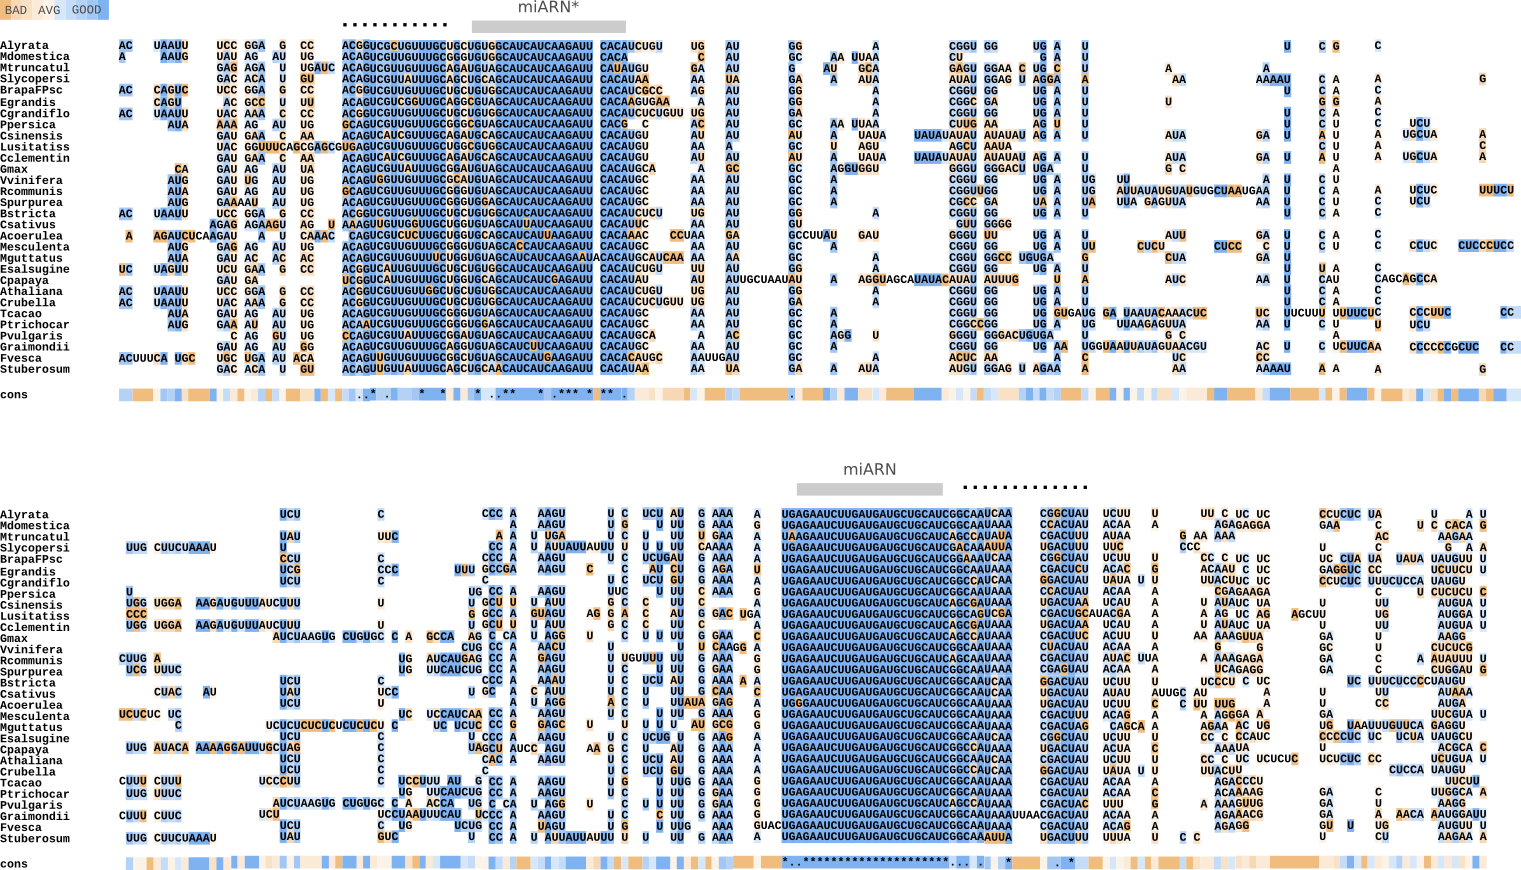
\includegraphics[width=1\textwidth]{img/miR172a_tcoffee_03.png}
	\end{center}
\end{frame}

\begin{frame}{Existe un patrón estructural que comparten los precursores, en la región inmediata por debajo del dúplex miARN/miARN*}
	\begin{center}
		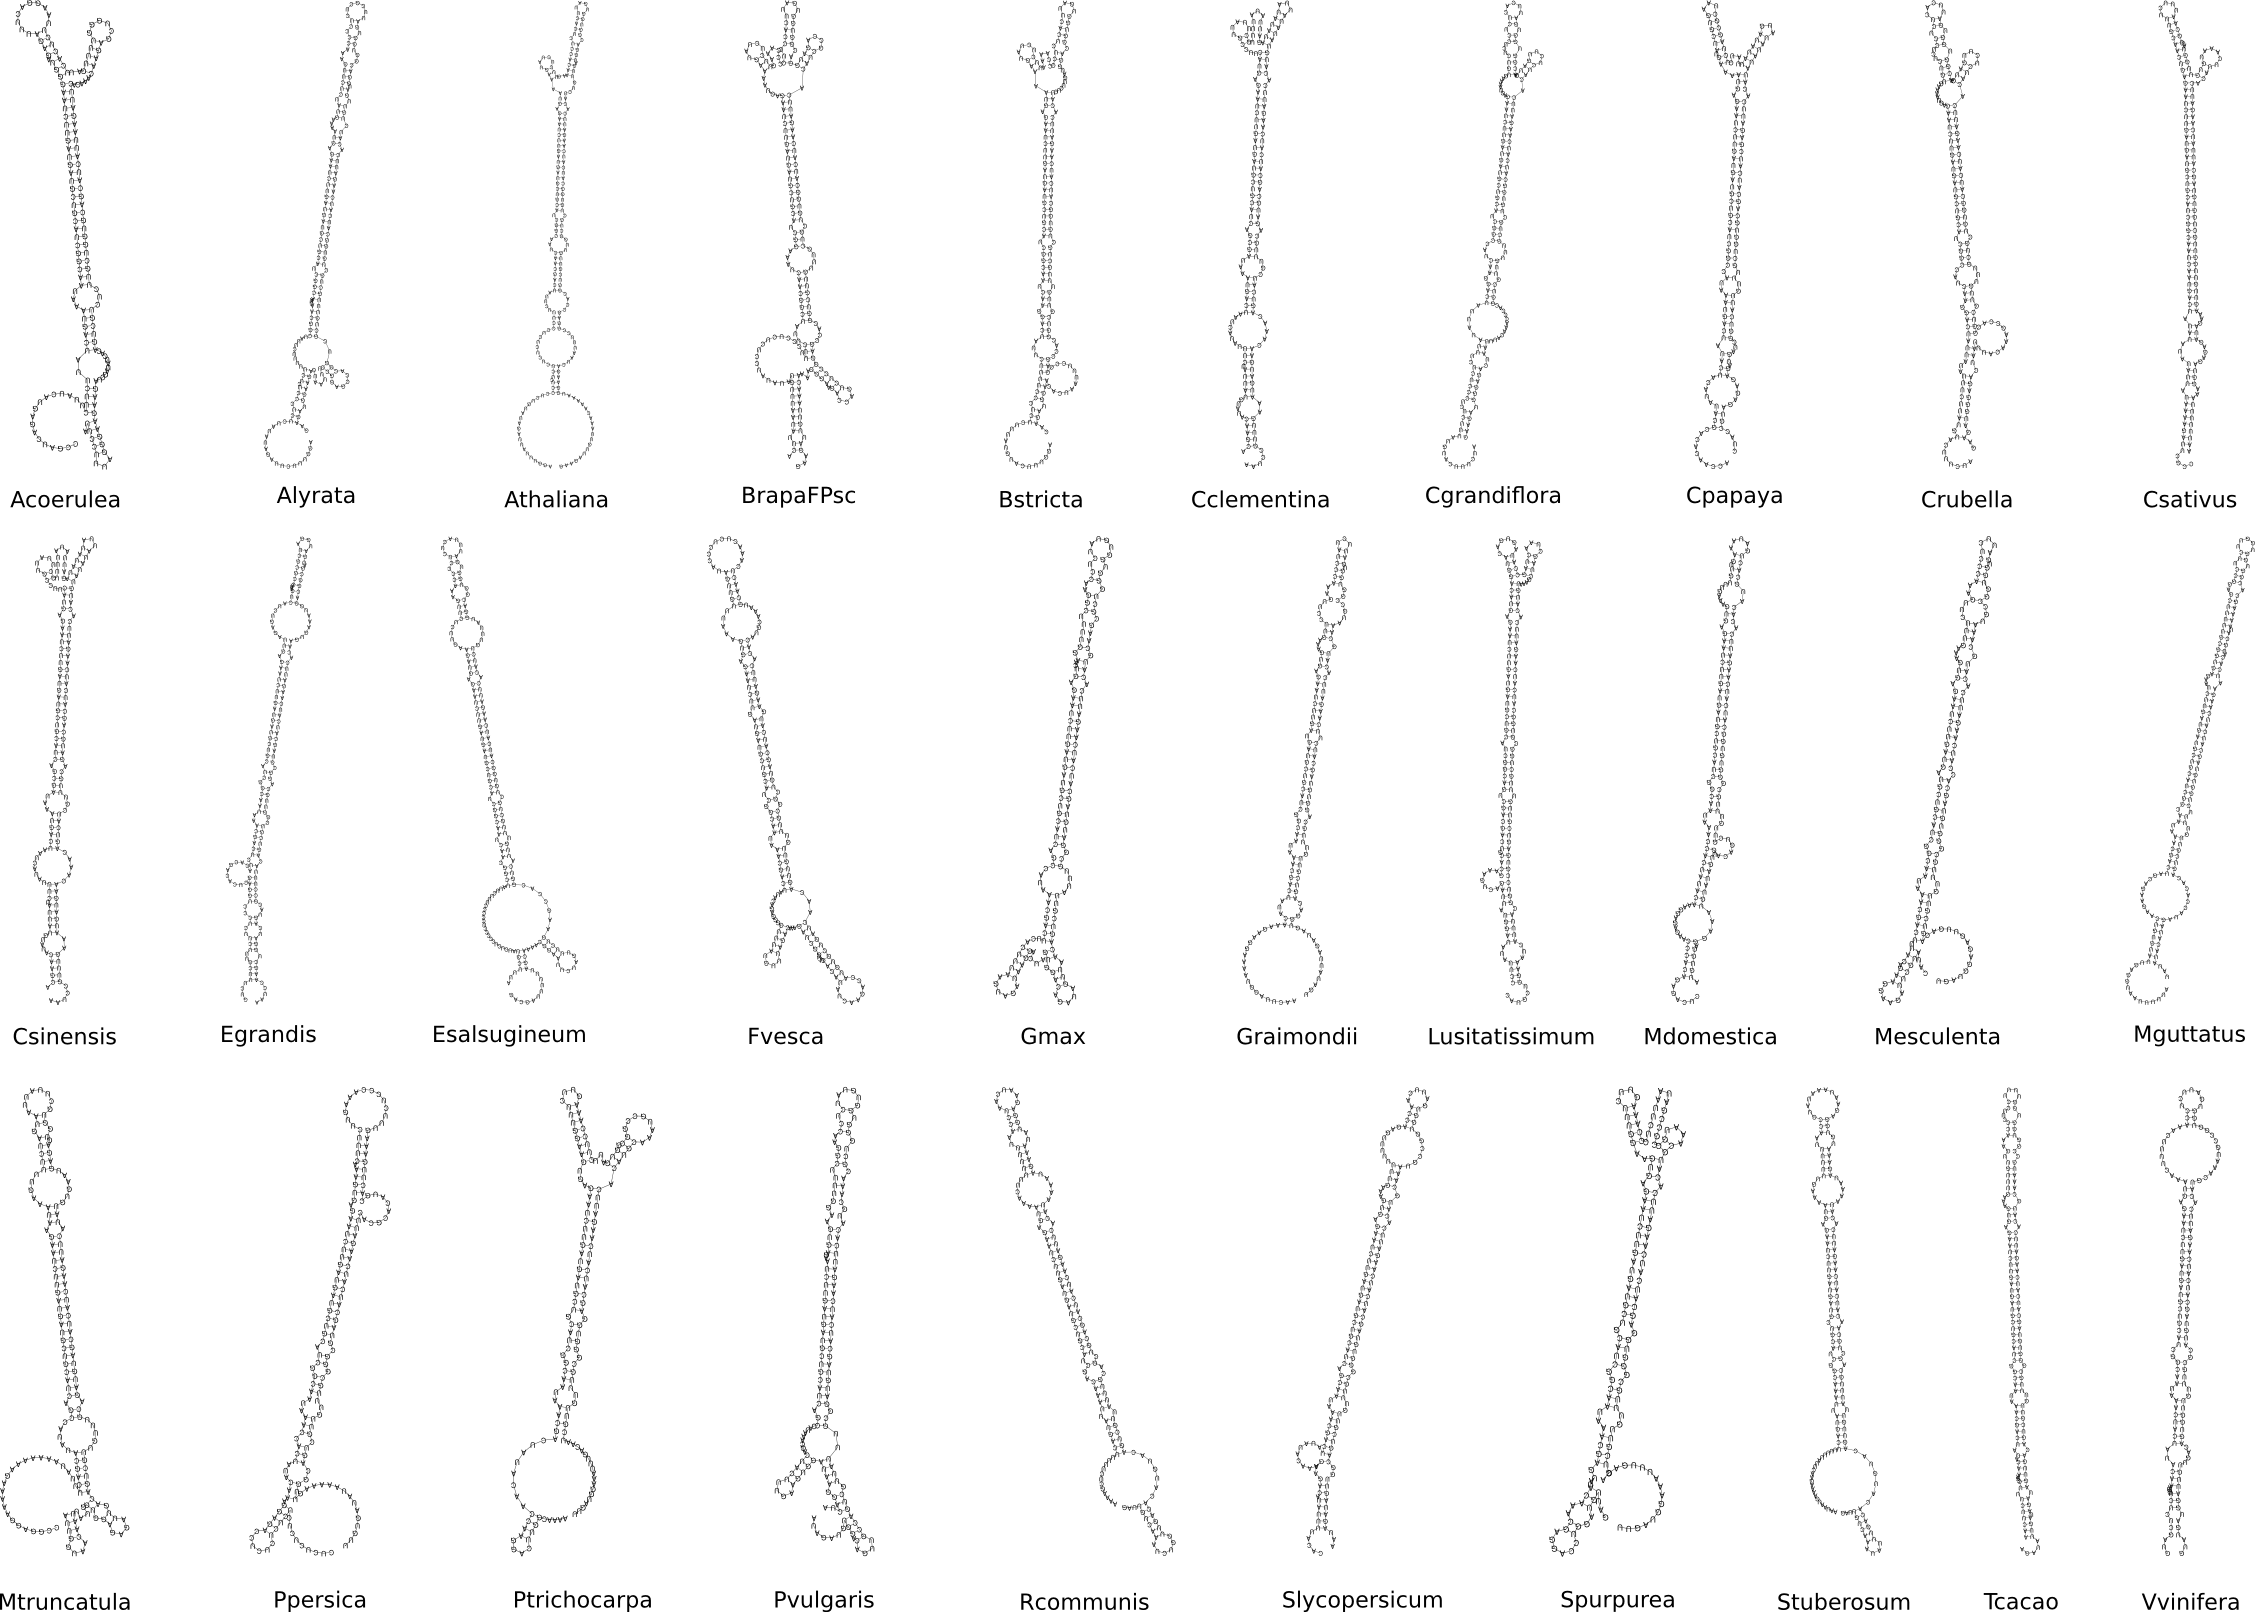
\includegraphics[width=.8\textwidth]{img/miR172a_rnafold.png}
	\end{center}
    \begin{center}
        \uncover<2->{No es trivial deducir información concreta a partir de estas figuras.}
    \end{center}
\end{frame}

\begin{frame}{Conservación del consenso en base al alineamiento de secuencia primaria}
	\begin{center}
		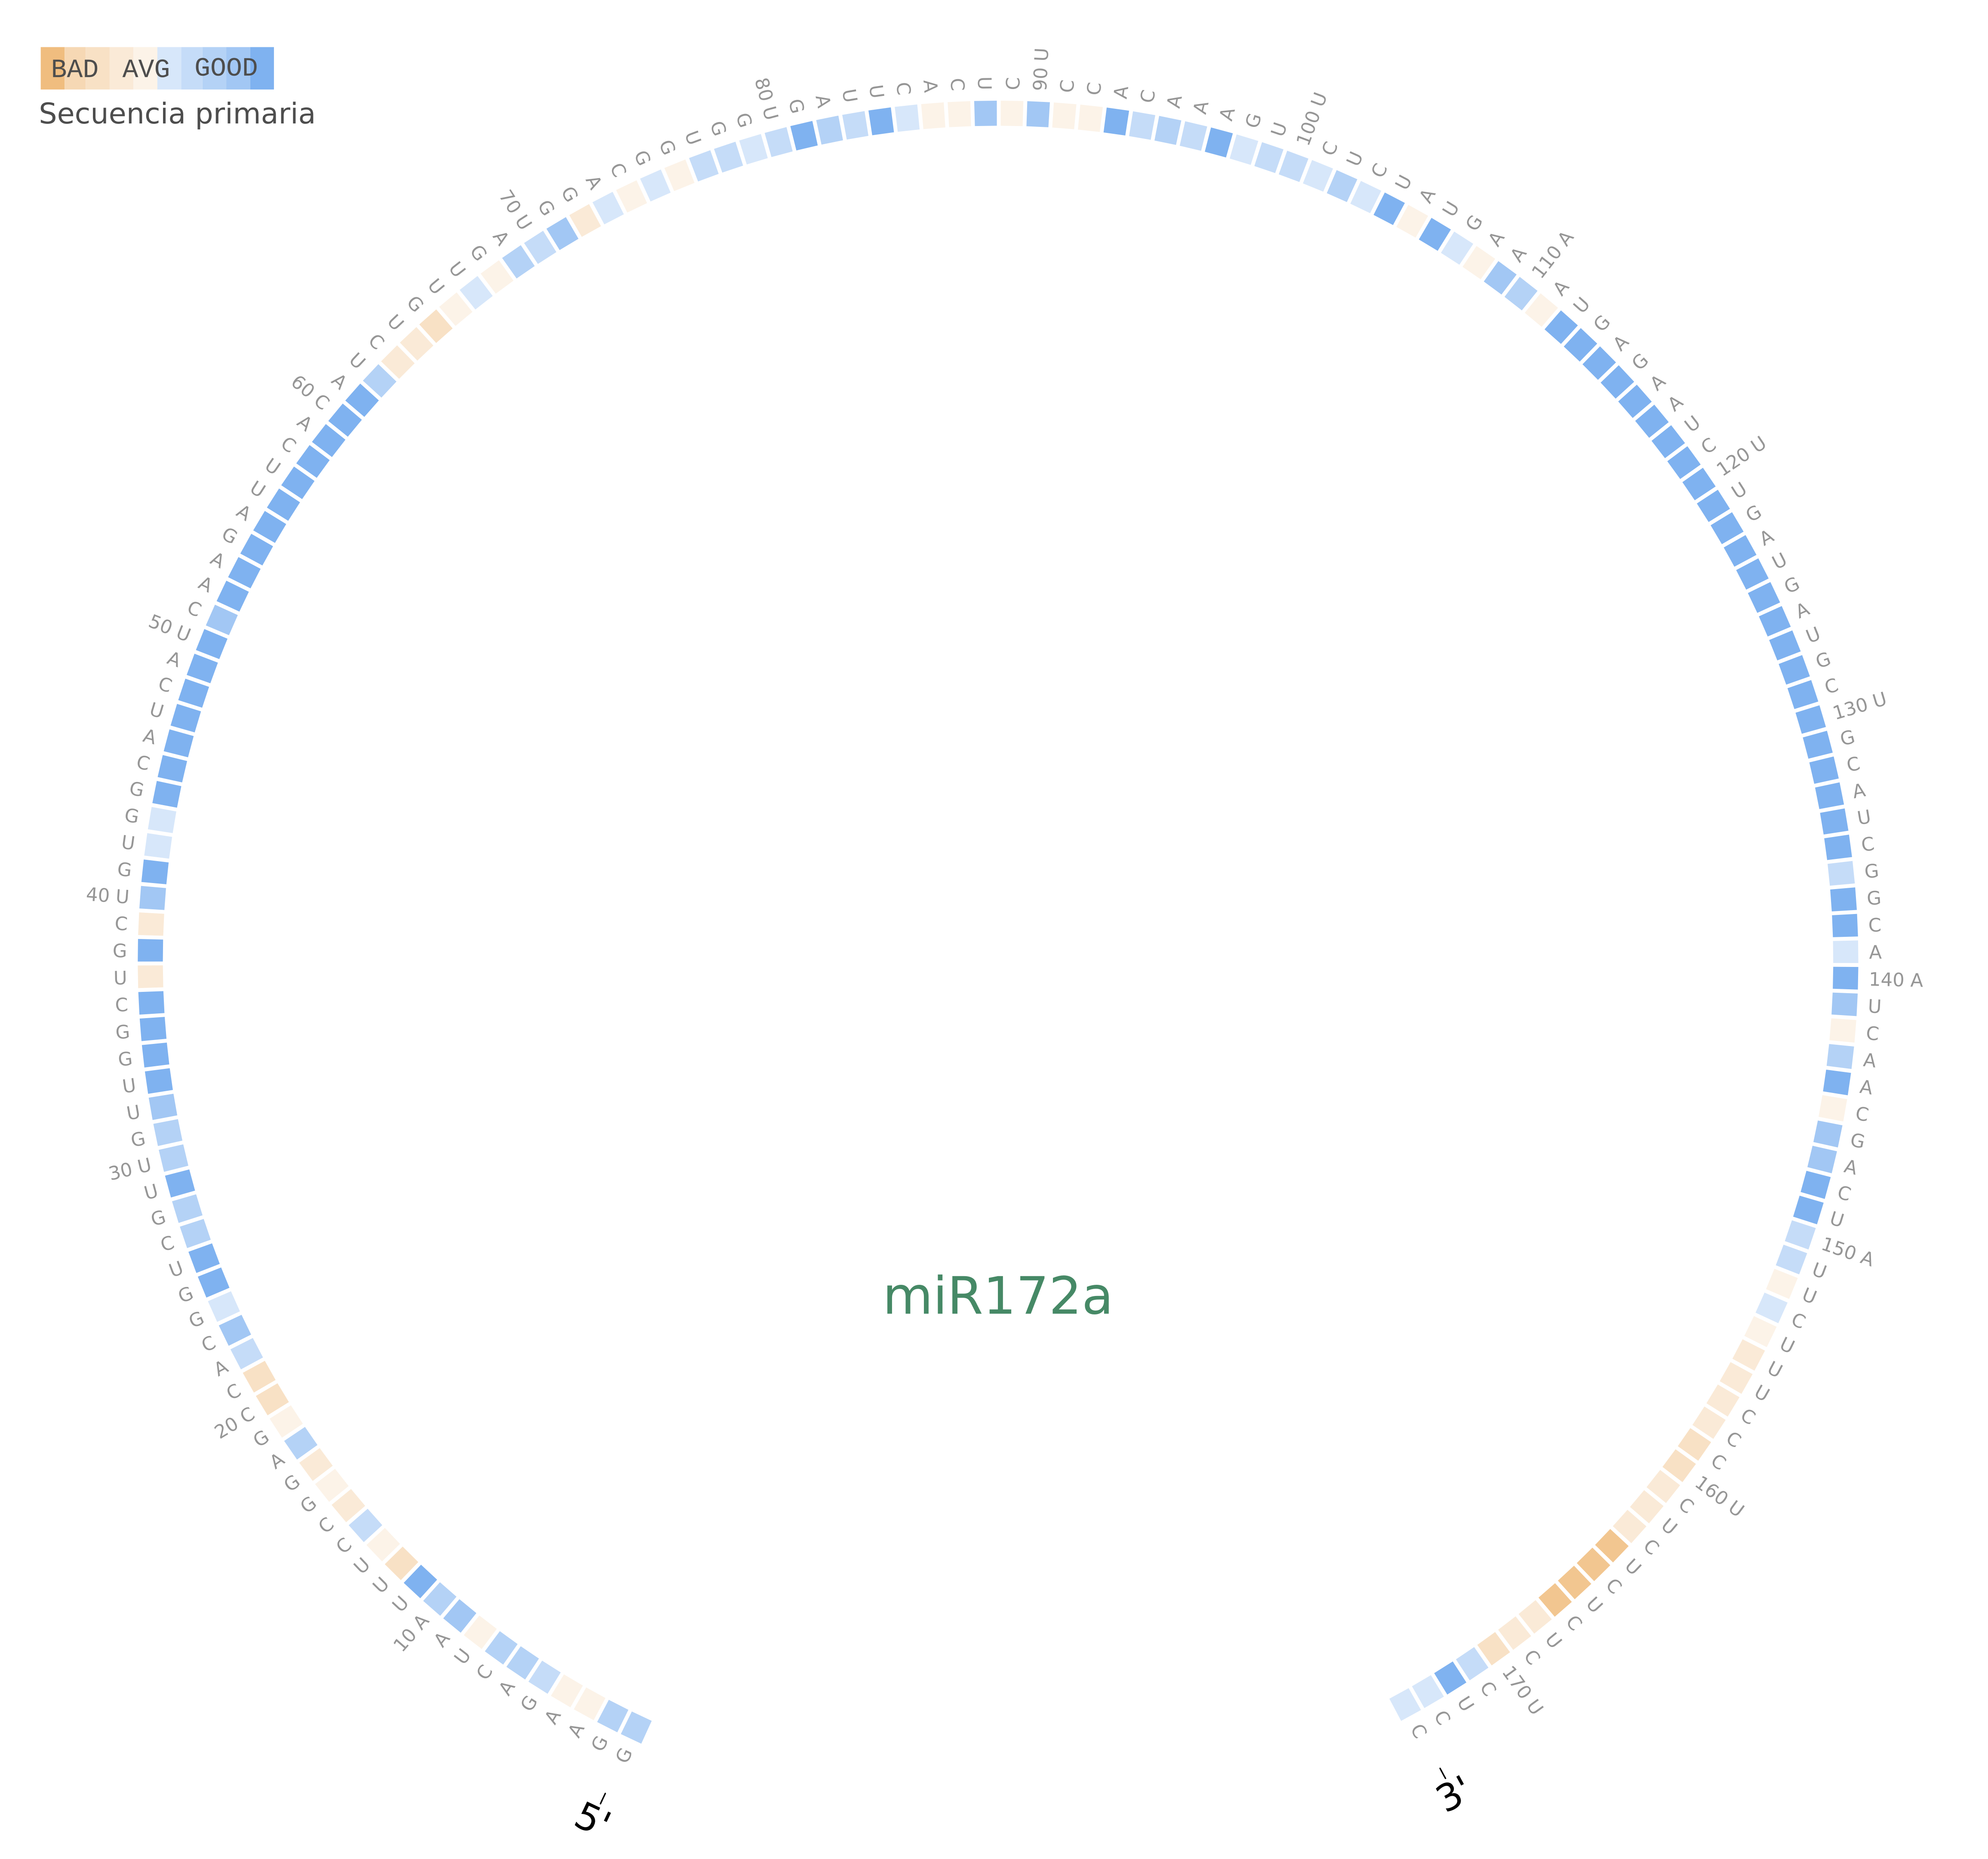
\includegraphics[width=.8\textwidth]{img/miR172a_circos01.png}
	\end{center}
\end{frame}

\begin{frame}{Frecuencia de bases apareadas y desapareadas}
	\begin{center}
		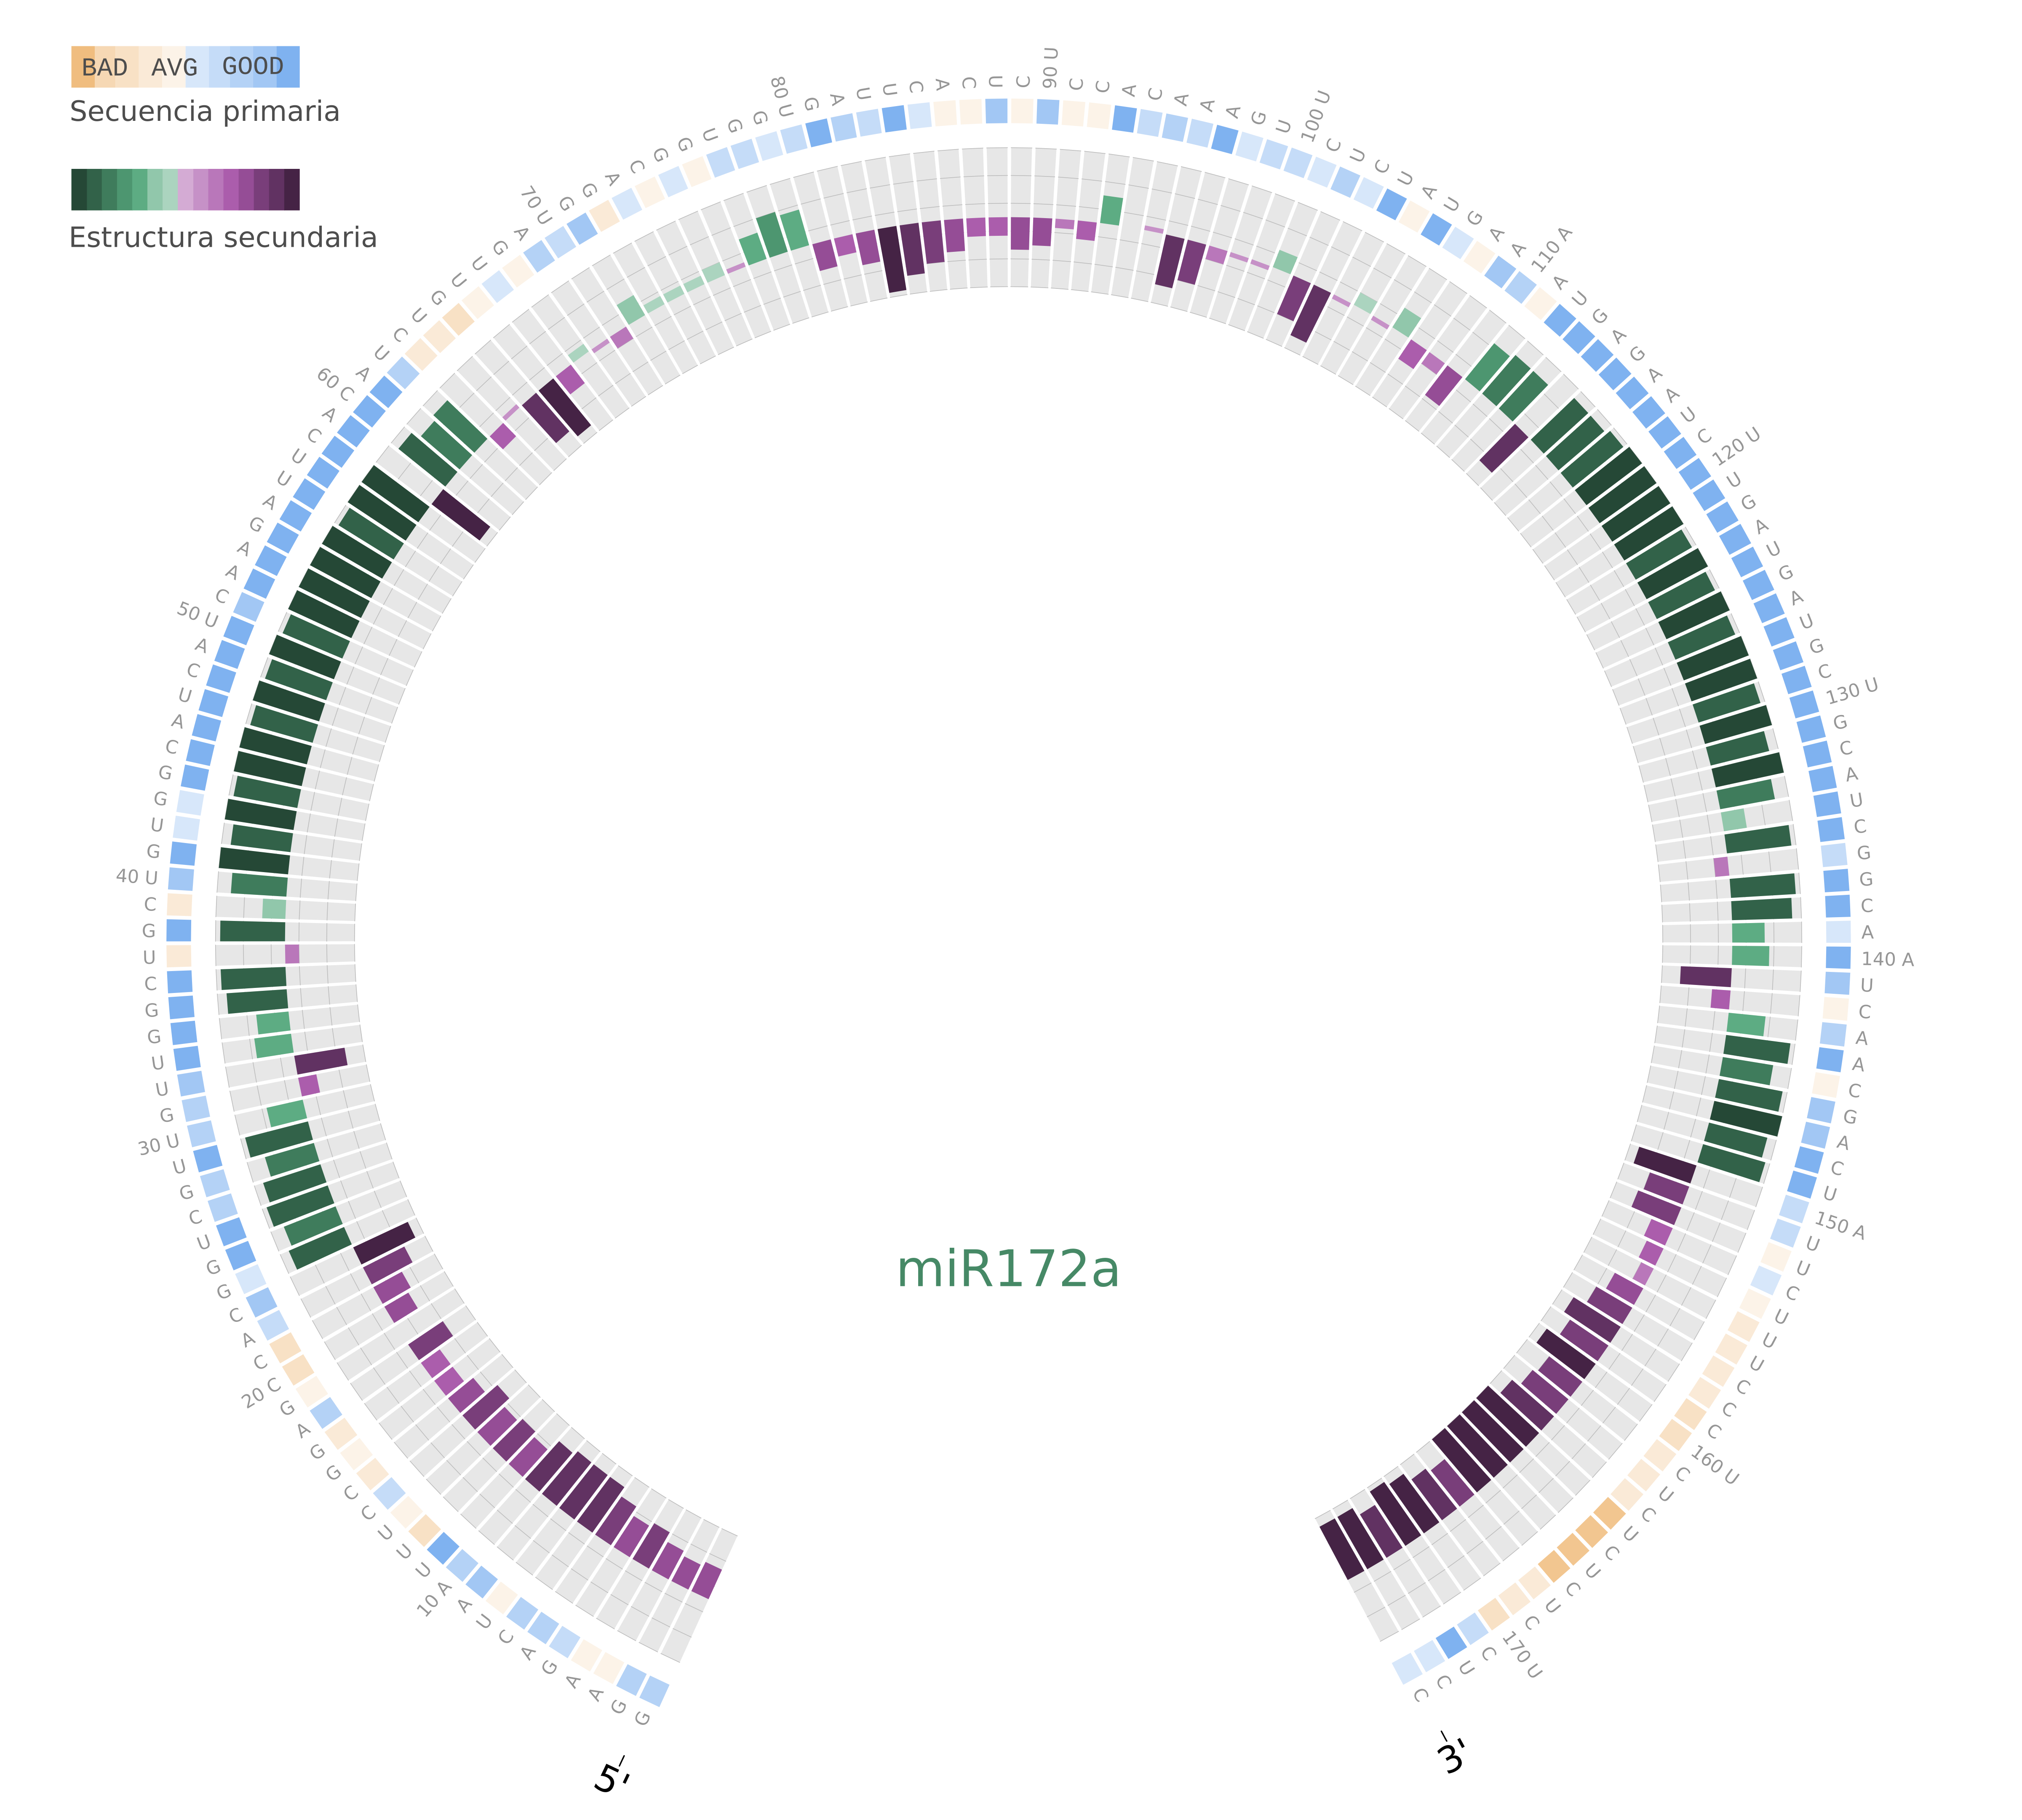
\includegraphics[width=.8\textwidth]{img/miR172a_circos02.png}
	\end{center}
\end{frame}

\begin{frame}{Interacción entre pares de bases considerando estructura secundaria}
	\begin{center}
		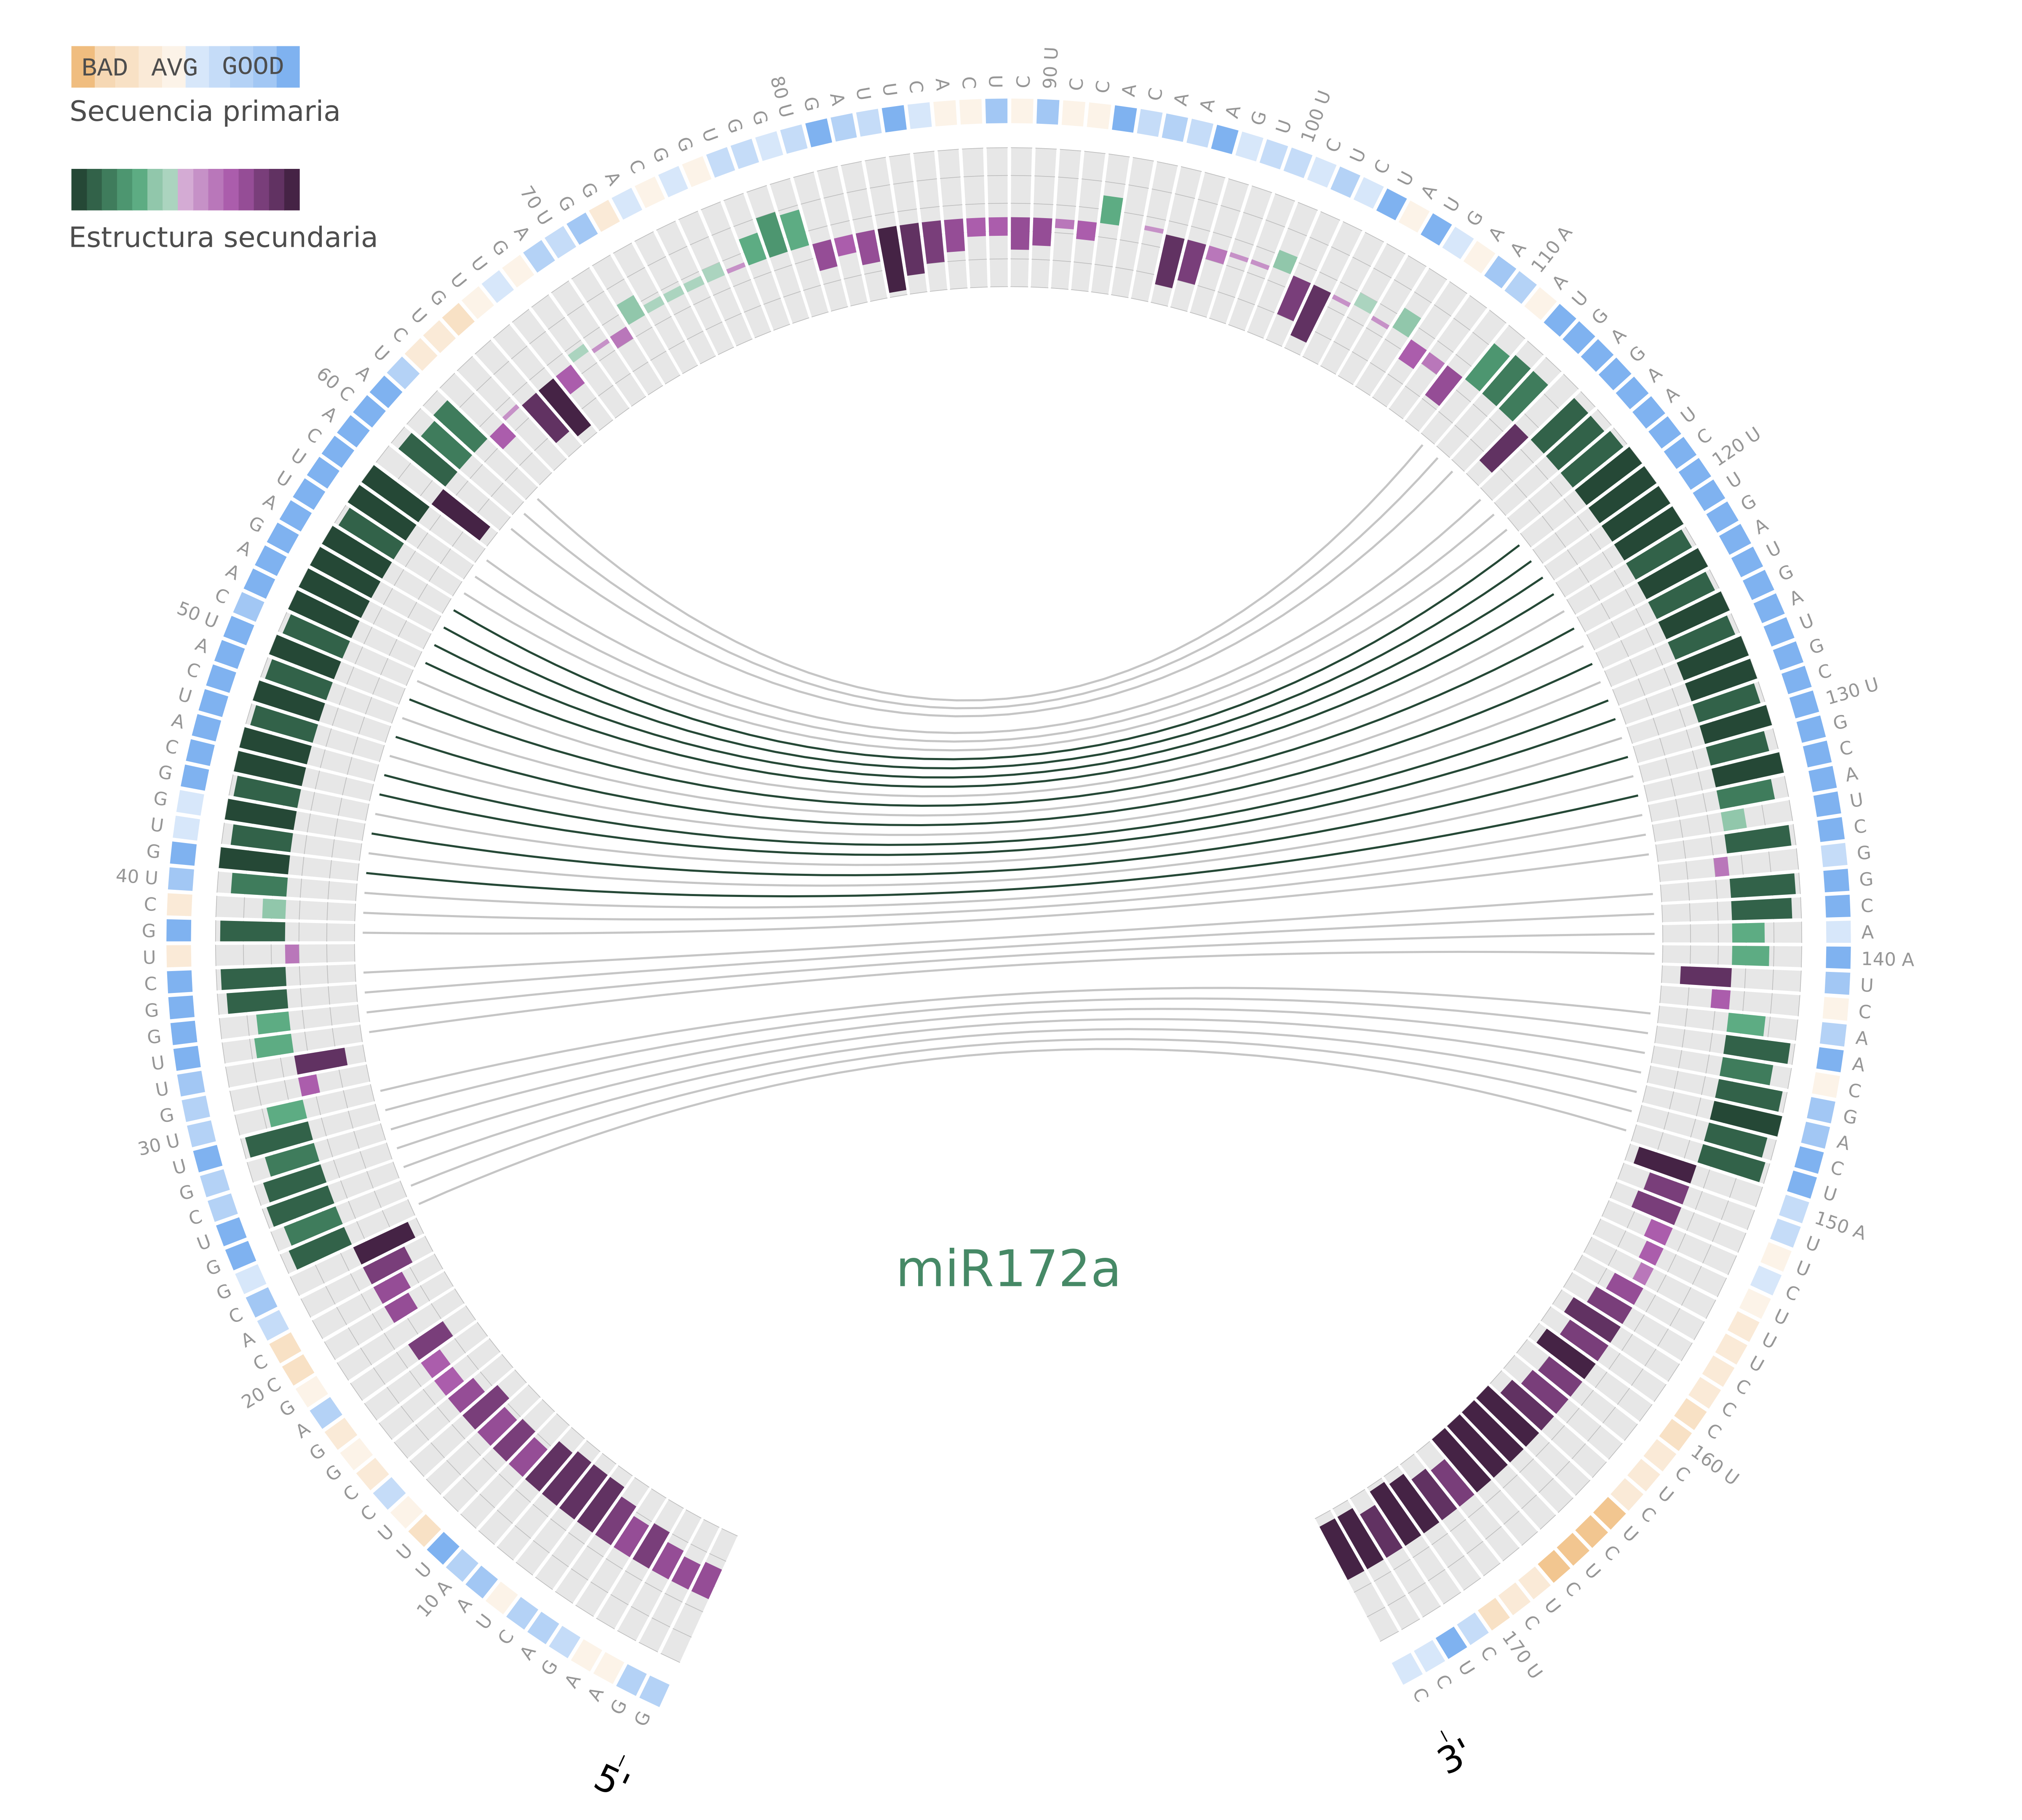
\includegraphics[width=.8\textwidth]{img/miR172a_circos03.png}
	\end{center}
\end{frame}

\begin{frame}{miARN y miARN* conservados en secuencia primaria y estructura}
	\begin{center}
		\includegraphics[width=.8\textwidth]{img/miR172a_circos04.png}
	\end{center}
\end{frame}

\begin{frame}{Región conservada por debajo del dúplex que coincide con el tallo inferior}
	\begin{center}
		\includegraphics[width=.8\textwidth]{img/miR172a_circos05.png}
	\end{center}
\end{frame}

\begin{frame}{Mismatches conservados}
	\begin{center}
		\includegraphics[width=.8\textwidth]{img/miR172a_circos06.png}
	\end{center}
\end{frame}

\begin{frame}{Mismo patrón de conservación en otros precursores que se procesan desde la base}
	\begin{center}
		\includegraphics[width=.8\textwidth]{img/miR390a_circos_defensa.png}
	\end{center}
\end{frame}

\begin{frame}{Precursores que se procesan desde la base en forma secuencial}
	\begin{center}
		\includegraphics[width=1\textwidth]{img/seqBTL_circos_defensa.png}
	\end{center}
\end{frame}

\begin{frame}{Precursores que se procesan desde el loop cortos}
	\begin{center}
		\includegraphics[width=1\textwidth]{img/srLTB_circos_defensa.png}
	\end{center}
\end{frame}

\begin{frame}{Precursores que se procesan desde el loop en forma secuencial}
	\begin{center}
		\includegraphics[width=1\textwidth]{img/seqLTB_circos_defensa.png}
	\end{center}
\end{frame}

\begin{frame}{En precursores que se procesan desde el loop, el tamaño de la región que comprende al tallo superior y al loop no varía en distintas especies}

	\begin{center}
		\includegraphics[width=.8\textwidth]{img/miR160a_meme.png}
	\end{center}
\end{frame}

\begin{frame}{En precursores que se procesan desde la base, el tamaño de la región que comprende al tallo superior y al loop es muy variado en distintas especies}
	\begin{center}
		\includegraphics[width=1\textwidth]{img/miR172_meme.png}
	\end{center}
\end{frame}

\begin{frame}{Procesamiento mixto de miembros de la familia del miR170/miR171}
	\begin{center}
		\includegraphics[width=1\textwidth]{img/familia_miR171_circos.png}
	\end{center}
\end{frame}

\begin{frame}{Mutaciones puntuales que afectan el procesamiento de miARNs en plantas}
	\begin{center}
		\includegraphics[width=.7\textwidth]{img/miR164_ss_bp.png}
	\end{center}
\end{frame}

\begin{frame}{Posición *2 del miR164a* está conservada  en dicotiledóneas}
	\begin{center}
		\includegraphics[width=.8\textwidth]{img/miR164a_circos.png}
	\end{center}
    \begin{center}
        \uncover<2->{La posición *2 es importante para la estabilidad del precursor y su buen procesamiento.}
    \end{center}
\end{frame}

\begin{frame}{Alelo mir394b-1 con un ``mismatch'' en el tallo inferior del precursor del miR394b}
	\begin{center}
		\includegraphics[width=.8\textwidth]{img/miR394b_circos_aliniamientos.png}
	\end{center}
    \begin{center}
        \uncover<2->{Mutaciones simples en el precursor puede afectar el reconocimiento de DICER.}
    \end{center}
\end{frame}


%~ IMPORTANTE
%~ Esta información también podría ser utilizada para ayudar en el diseño de miARNs artificiales en distintas especies y aumentar su eficiencia


\begin{frame}{Variante del miR396 específica de monocotiledóneas}
	\begin{center}
		\includegraphics[width=.8\textwidth]{img/circos_monocots_miR396e_defensa.png}
	\end{center}
    \begin{center}
        \uncover<2->{El nucleótido extra, que le da identidad a la variante de monocotiledóneas, está conservado.}
    \end{center}
\end{frame}


\begin{frame}{¿Qué sucede con los precursores de miARNs conservados en animales?}
\begin{table}[]
    \centering
    \tiny
    \begin{tabular}{c}
    \textbf{Animales}        \\
        Bos taurus               \\
        Canis familiaris         \\
        Equus caballus           \\
        Gallus gallus            \\
        Gorilla gorilla          \\
        Homo sapiens             \\
        Macaca mulatta           \\
        Monodelphis domestica    \\
        Mus musculus             \\
        Ornithorhynchus anatinus \\
        Petromyzon marinus       \\
        Sus scrofa               \\
        Xenopus tropicalis      
    \end{tabular}
    \end{table}
\end{frame}

%~ \begin{frame}{
%~ hsa-let-7-a.
%~ \uncover<2->{El loop terminal está conservado en la mayoría de los precursores de animales estudiados.}
%~ }
    %~ \begin{center}
        %~ La riboproteína HnRNP A1 se une al loop terminal del precursor de let-7-a e inhibe su procesamiento por Drosha.
    %~ \end{center}
	%~ \begin{center}
		%~ \uncover<2->{\includegraphics[width=.6\textwidth]{img/hsa-let-7a-1_circos.png}}
	%~ \end{center}
%~ \end{frame}

\begin{frame}{
El loop terminal está conservado en la mayoría de los precursores de animales estudiados.}
	\begin{center}
		\includegraphics[width=.8\textwidth]{img/hsa-let-7a-1_circos_defensa.png}
	\end{center}
\end{frame}


%~ % ACA TENGO QUE VER BIEN COMO DECIR LAS COSAS

\begin{frame}{Circos animales vs plantas}
	\begin{center}
		\includegraphics[width=1\textwidth]{img/animals_vs_plants_circos_defensa.png}
	\end{center}
        %~ Aca tengo que decir:
            %~ los prec en plantas que se procesan de abajo tienen conservación hacia abajo
            %~ los prec en plantas que se procesan de arriba tienen conservación hacia arriba
            %~ en animales: cons abajo -> corte por drosha
            %~ arriba -> exporte al citoplasma
            %~ en plantas esto no existe al ser procesado en forma nuclear
\end{frame}


\begin{frame}{Conclusiones III}
	\begin{itemize}
        \item<1-> Presentamos un enfoque bioinformático para el estudio de la evolución y biogénesis de miARNs en plantas.
        \item<2-> Desarrollamos una implementación gráfica para visualizar de manera simple los precursores de miARNs en distintas especies de plantas.
        \item<3-> Lo utilizamos para caracterizar la evolución de precursores de miARNs en plantas con distintos mecanismos de procesamiento.
        \item<4-> Estudiamos precursores con mutaciones que afectan al procesamiento de miARNs en plantas. 
        Esta información podría ser utilizada para ayudar en el diseño de miARNs artificiales en distintas especies y aumentar su eficiencia.
        \item<5-> Pudimos utilizar este mismo enfoque para estudiar precursores de miARNs en animales.
	\end{itemize}
\end{frame}

\section{Conclusiones generales}

\begin{frame}{Conclusiones generales}
	\begin{itemize}
        \item<1-> Desarrollamos aplicaciones bioinformáticas para el estudio de interacciones miARN-gen blanco.
        %~ \item<2-> Desarrollo de la herramienta comTAR
        \item<2-> Encontramos determinantes mecanísticos del procesamiento de miARNs en plantas.
        \item<3-> Desarrollamos una herramienta para el análisis de bibliotecas de SPARE incluyendo una interfaz gráfica.
        \item<4-> Analizamos las estructuras de los precursores y su evolución.
        \item<5-> Realizamos una forma de representación Visualización de información compleja por adaptación de una herramienta Circos.
    \end{itemize}
\end{frame}

    %~ \vspace{1cm}

\begin{frame}{}
	\begin{center}
		\Huge Muchas gracias.
	\end{center}
\end{frame}

\begin{frame}{}
	\begin{center}
	\end{center}
\end{frame}

\begin{frame}{}
	\begin{center}
		\includegraphics[width=.5\textwidth]{img/extras/NAR_fig3A.png}
	\end{center}
\end{frame}

\begin{frame}{}
	\begin{center}
		\includegraphics[width=.5\textwidth]{img/extras/NAR_fig3B.png}
	\end{center}
\end{frame}

\begin{frame}{Nuevos genes blancos validados en \textit{A. thaliana}}
	\begin{center}
		\includegraphics[width=1\textwidth]{img/Figure4_retocada.png}
	\end{center}
\end{frame}

\begin{frame}{Nuevos genes blancos con interacciones G-U}
	\begin{center}
		\includegraphics[width=.6\textwidth]{img/Figure5_retocada.png}
	\end{center}
\end{frame}

\begin{frame}{Tallo inferior de 15 nt en precursores procesados desde la base}
	\begin{center}
		\includegraphics[width=1\textwidth]{img/GR_fig2C.png}
	\end{center}
\end{frame}

\begin{frame}{Región terminal estructurada en precursores procesados desde el loop}
	\begin{center}
		\includegraphics[width=1\textwidth]{img/GR_fig4C.png}
	\end{center}
\end{frame}

\end{document}
